%% Arbitrum DAO Governance — Main Paper
%% Journal of Finance formatting
%% Compile: pdflatex main.tex && bibtex main && pdflatex main.tex && pdflatex main.tex

\documentclass[12pt]{article}

%% ── Packages ──────────────────────────────────────────────────────────────────
\usepackage[margin=1in]{geometry}
\usepackage{setspace}
\usepackage{times}
\usepackage{lmodern}
\usepackage{natbib}
\usepackage{amsmath,amssymb,amsthm}
\usepackage{booktabs}
\usepackage{graphicx}
\usepackage{float}

\newtheorem{proposition}{Proposition}
\newtheorem{lemma}{Lemma}
\renewcommand{\qedsymbol}{}
% Compact captions: small font, bold label, tighter vertical spacing
\setlength{\abovecaptionskip}{5pt}
\setlength{\belowcaptionskip}{2pt}
\makeatletter
\renewcommand{\@makecaption}[2]{%
  \vskip\abovecaptionskip
  \sbox\@tempboxa{{\small\textbf{#1:} #2}}%
  \ifdim \wd\@tempboxa >\hsize
    {\small\textbf{#1:} #2\par}%
  \else
    \global\@minipagefalse
    \hb@xt@\hsize{\hfil\box\@tempboxa\hfil}%
  \fi
  \vskip\belowcaptionskip}
\makeatother
% \@currentlabel is set locally inside \caption's singlespace group; make it global
% so that \label commands placed outside \begin{singlespace} still capture the figure number.
\makeatletter
\let\latex@refstepcounter\refstepcounter
\renewcommand\refstepcounter[1]{%
  \latex@refstepcounter{#1}%
  \global\let\@currentlabel\@currentlabel
}
\makeatother
% FloatBarrier: outputs pending floats at subsection boundaries without a hard page break
\newcommand{\FloatBarrier}{\par}
\usepackage[hypertexnames=false]{hyperref}
\usepackage{xcolor}
\usepackage[T1]{fontenc}

\hypersetup{
  colorlinks=true,
  linkcolor=black,
  citecolor=black,
  urlcolor=black
}

\doublespacing

\newcommand{\sym}[1]{\ifmmode^{#1}\else\(^{#1}\)\fi}
\newcommand{\specialcell}[2][c]{\begin{tabular}[#1]{@{}l@{}}#2\end{tabular}}

%% ── Title ─────────────────────────────────────────────────────────────────────
\title{\textbf{The Effect of AI Writing on Governance: Evidence from a \$3.5 Billion DAO}}

\author{
  Victor Huang$^{*}$ \and Joseph Hall$^{*}$
  \\[0.5em]
  \small $^{*}$Georgia Institute of Technology
}

\date{\today}

\begin{document}

\maketitle
\vspace{-1.5em}

\begin{singlespace}
\begin{abstract}
\noindent
We study the extent to which online deliberation aggregates information before collective votes.
Our setting is Arbitrum DAO, a decentralized organization controlling a \$3.5 billion treasury, where token holders debate proposals on a public forum before each binding vote.
Forum activity predicted vote closeness before March 2024 but became uninformative after, coinciding with language models capable of producing indistinguishable governance prose.
Interestingly, we observe that the degradation of the forum's signal (the elimination of the correlation between posting volume and margin-of-victory) takes place at a time when relatively few posts are A.I.\ generated, relative to the end of the sample period where A.I.\ posting volume grows rapidly.
We use a model of endogenous posting and voting to show that this may be a general phenomenon: the signal value of the forum can collapse to zero at a discrete tipping point with a very low volume of A.I.\ posts.
Calibrating to the data, the forum generated net social benefits equivalent to saving at least 858 words of research effort per delegate per proposal---all destroyed at the tipping point.
Delegates who rely on AI hold far less voting power than those who do not, ruling out power capture by insiders.
Our results suggest that the mere existence of indistinguishable AI writing is sufficient to degrade the governance capabilities of economically important organizations, even if such AI is rarely used in equilibrium.
\end{abstract}

\vspace{0.3em}
\noindent\textit{JEL}: G18, G34, D72, O33\quad
\noindent\textit{Keywords}: decentralized autonomous organizations, DAO governance,
artificial intelligence, information aggregation, structural break, blockchain governance
\end{singlespace}

\clearpage

%% ── 1. Introduction ───────────────────────────────────────────────────────────
\section{Introduction}
\label{sec:intro}

%% [DRAFT — see sections/introduction.tex]

% --- sections/introduction ---
Text-based deliberation is a foundation of financial governance. The Securities
and Exchange Commission solicits public comment before finalizing rules and treats
letter volume and content as a gauge of genuine stakeholder concern. Shareholders
read proxy statements, activist letters, and analyst reports before contested votes
on mergers, compensation, and board composition \citep{iliev2015}. Retail investors
post on Reddit and StockTwits, and a large empirical literature has established that
this crowd activity carries real information about market outcomes
\citep{antweiler2004, chen2014}. The informational value of each of these mechanisms
rests on a single implicit assumption: that producing credible, contextually
appropriate long-form prose requires genuine expertise or conviction---a cost
sufficient to screen out noise and make text a credible signal of authentic opinion.

Artificial intelligence is destroying that assumption. As the marginal cost of
generating sophisticated, indistinguishable prose approaches zero, the link between
text production and genuine information is severed---and with it, the credibility of
every text-based deliberation channel in finance. This paper asks how fast the
collapse happens, what triggers it, and why. Our laboratory is the Arbitrum DAO
governance forum: a real-money governance setting with \$3.5 billion in treasury
assets, with every post and vote recorded immutably on blockchain, and---because crypto
communities are technically sophisticated and move faster than traditional capital
markets---the first financial governance context to confront the AI quality threshold
at scale---and therefore the first setting in which the mechanism we study can
be cleanly identified. What we find here is likely to recur in corporate earnings
calls, analyst forums, and any other text-based financial deliberation as AI
capability continues to advance.

We study this question using a setting that provides what corporate governance
research rarely enjoys: an exogenous shock to the quality of the signal. On March 4,
2024, Anthropic released Claude~3, a large language model capable of producing
sophisticated, contextually appropriate long-form prose. Within weeks, the
Arbitrum governance forum---like most online platforms---experienced a wave of
AI-generated posts. These posts are grammatically fluent, topically relevant, and
superficially indistinguishable from human-authored contributions. They are not,
however, opinion-bearing: they do not reflect a genuine preference for or against the
proposal in question, and they do not aggregate private information held by
stakeholders. They carry no directional vote signal: they do not predict whether a proposal passes or fails.

We measure AI-generated content using the Pangram API, a commercial AI-detection
service that returns, for each post, the estimated fraction of content generated by
large language models (\textit{fraction\_ai}). We classify posts with
\textit{fraction\_ai}~$>0.70$ as AI-written and posts below this threshold as
human-written. This classification allows us to separately track the human signal and
the AI noise within each proposal thread across the full sample period.

Our main finding is a structural break. In the pre--Claude~3
period (January 2023 through February 2024), the number of human-authored posts in a
proposal's forum thread predicts the proposal's margin of
victory---the absolute difference in vote share between the winning and losing
sides among contested (For vs.\ Against) votes. The Pearson correlation is
$r = -0.33$ ($p = 0.08$, $n = 29$ proposals): more posts, more disagreement,
smaller margin. This is consistent with a forum that aggregates genuine signals
of community sentiment. Delegates and token holders who observe an unusually active
thread are, in effect, observing a sufficient statistic for the degree of community
division.

After Claude~3, this relationship vanishes. The correlation falls to $r = -0.10$
($p = 0.39$, $n = 73$) in the post-shock period. The change in the correlation
coefficient, $\Delta r = +0.23$, is confirmed by a
Chow test that rejects parameter stability at $F = 8.38$ ($p = 0.0004$). We use Claude~3 (March 2024) as our primary break date, which provides a clean before-and-after contrast. All substantive conclusions hold at any candidate break date from November 2023 onward (Table~\ref{tab:chow_battery}).

The identification logic rests on the exogeneity of AI capability releases. AI model
releases are global events determined by the research roadmaps of Anthropic, OpenAI,
and other technology companies---they are plainly exogenous to any specific Arbitrum
proposal. The release of Claude~3 was not anticipated by the Arbitrum community, was
not timed to coincide with any particular governance vote, and affected all future
proposal threads uniformly. The shock therefore provides a plausible source of
quasi-exogenous variation in the posting environment. We interpret the before--after
comparison as the best available quasi-experimental evidence consistent with an
AI-contamination mechanism. We acknowledge that the November 2023--March 2024 window
also encompasses several concurrent governance developments---LTIPP/STIP grant batching,
the approach of the March 2024 token vesting cliff, and expanding vote-rental
participation---that could in principle affect the posts--margin relationship.
Section~\ref{sec:strategy} and the robustness checks in Section~\ref{sec:robustness}
evaluate each of these alternatives directly. Cross-DAO evidence
(Figure~\ref{fig:participation}) provides additional corroboration: five major DeFi
DAOs without Arbitrum-specific governance dynamics exhibit comparable participation
declines over the same window, inconsistent with Arbitrum-specific confounders as
the primary driver.

We then turn to the mechanism. The most natural candidate explanation---that a
physical flood of AI-generated posts numerically overwhelmed the human signal---is
falsified by timing. To be precise: AI-generated posts are detectable on the forum
well before the structural break---a small but measurable share appear as early as
early 2023---but at negligible volume. At the date of the QLR break (November 2023),
AI posts constituted approximately 8\% of forum volume, and approximately 6\% at the Claude~3 break (March 2024)---remaining in the single digits throughout, and dipping below 3\% in between. The large-scale volume surge did not arrive until late 2024, reaching 15--20\% of forum traffic nine to twelve months after the signal collapsed. A volume mechanism requires contamination to precede collapse; the data show the reverse.

We propose instead an \emph{unverifiability shock} mechanism in the spirit of
\citet{akerlof1970}. The releases of GPT-4 Turbo (November 2023) and Claude~3
(March 2024) crossed a quality threshold at which AI-generated governance prose
became indistinguishable from careful human writing.

There is direct benchmark evidence that these two releases were qualitatively different from their predecessors. On the Massive Multitask Language Understanding benchmark \citep[MMLU;][]{hendrycks2021}, which tests breadth of knowledge across 57 academic and professional domains, GPT-4 (March 2023) scored 86.4\% versus 70.0\% for GPT-3.5---a step change that closed most of the remaining gap to expert human performance (estimated at 89.8\%). GPT-4 Turbo extended this to 87.3\%, and Claude~3 Opus reached 86.8\% \citep{anthropic2024}. On MT-Bench, a benchmark designed to evaluate multi-turn instruction-following and writing quality, GPT-4 achieved a score of 8.99 out of 10 versus 7.94 for GPT-3.5 \citep{zheng2023}.

Two further lines of evidence, neither reliant on vendor-reported benchmarks, corroborate that this generation crossed a human-indistinguishability threshold. First, blind human preference: on the LMSYS Chatbot Arena, where users vote on anonymized head-to-head outputs \citep{zheng2023}, Claude~3 Opus (released March 4, 2024) became the first non-OpenAI model to overtake the GPT-4 family at the top of the leaderboard, which GPT-4 variants had led since May 2023; earlier models such as Claude~2 never reached that tier. Second, controlled Turing tests: in a randomized, preregistered two-party test, \citet{jones2024turing} found GPT-4 judged to be human 54\% of the time---versus 66--67\% for real humans and 22\% for a 1960s \textsc{eliza} baseline---up from 49.7\% for the best GPT-4 prompt in an earlier online study \citep{jones2023turing} and near-chance for prior models, and a subsequent three-party test reached 73\% for GPT-4.5, above the human baseline \citep{jones2025turing}. These are ordinal claims established by blind human judgment rather than self-reported capability scores, and they place the crossing of near-human indistinguishability in the November 2023--March 2024 window (Figure~\ref{fig:turing}). We acknowledge two caveats: no benchmark measures indistinguishability of \emph{governance-forum} prose specifically, so the Arena and Turing tests are the nearest available instruments; and the highest Turing pass rates require prompting the model to adopt a humanlike persona.

Once this threshold was crossed,
governance delegates---who read forum posts as signals of community sentiment---could
no longer verify the authenticity of any given post. Under standard informational
logic \citep{grossman1980}, the expected value of an unverifiable signal falls toward
its prior: once the expected probability of AI contamination exceeds a threshold,
delegates rationally discount the forum even though realized contamination remains
low. The credible \emph{threat} of AI content is sufficient to destroy the forum's
information value---even before any flood of AI posts arrives.

Delegate-level evidence is consistent with this mechanism and rules out a power-capture
story. Using a dataset linking forum usernames to Snapshot voting
records for 62 delegates, we document a robust negative cross-sectional relationship
between a delegate's average AI content fraction and their average delegated voting
power: $r = -0.44$ ($p = 0.001$, $n = 51$ delegates). High-AI delegates hold on
average 71,000 ARB in delegated power; low-AI delegates average 1.9 million ARB---a
gap of 27$\times$. AI tools are adopted primarily by lower-tier delegates seeking
to maintain forum presence at lower cost, not by high-power insiders seeking to
manufacture consensus. The signal degrades not because the powerful are gaming the
forum, but because the \emph{possibility} of doing so at zero cost became credible.

We also examine whether the distraction hypothesis of \citet{hirshleifer2009}---in
which exogenous events that command attention reduce participation in other
activities---can account for variation in posting volume or vote outcomes. We
construct a comprehensive battery of candidate distraction instruments: major token
airdrops (ZKsync, LayerZero, Starknet), cryptocurrency market crashes (Bank of Japan
rate shock, August 2024; SVB collapse, March 2023), exchange hacks and security
incidents, regulatory events (SEC enforcement actions, Bitcoin ETF approval), and
concurrent DAO proposal load. Every instrument with a statistically significant
first stage has the \emph{wrong sign}: exogenous events increase, rather than
decrease, forum activity. This finding is itself informative about the nature of DAO
participation. Unlike the retail investors in \citet{hirshleifer2009}, Arbitrum DAO
participants are core stakeholders who treat DeFi market events as
\emph{complements} to governance engagement, not substitutes. This indicates that DAO governance involves a fundamentally different
mode of participation than the retail trading studied in the attention literature:
core stakeholders respond to market events by \emph{engaging more}, not tuning out.

\paragraph{Contributions.} This paper makes four contributions.

\emph{First}, we provide the first empirical evidence that online governance forums
aggregate genuine information about vote outcomes. The pre-shock posts--margin
relationship documents that forum activity is not epiphenomenal: it tracks real
community division in a way that has predictive content for on-chain vote outcomes.
This connects the DAO literature \citep{yermack2017, kiayias2022, barbereau2023}
to the social-media-and-markets literature \citep{antweiler2004, chen2014, cookson2020},
extending both to a setting where the forum is the public, recorded deliberation
channel between information and vote.

\emph{Second}, we provide the first quasi-experimental evidence on the effect of
AI-generated content on collective decision mechanisms. The AI shock literature
\citep{lopezlira2023, cao2023, brynjolfsson2023} has focused on effects on labor
markets and financial analysis; our contribution is to show that generative AI
degrades a specific form of information aggregation---democratic deliberation---through
a channel not studied in prior work: the collapse of participation costs reduces the cost of mimicking credible engagement.

\emph{Third}, we document the internal structure of the DAO delegate market. The
delegate system in Arbitrum and other major DAOs is a form of liquid democracy
\citep{blum2016, green2015}: token holders delegate their voting power to
representatives who specialize in governance participation. We provide the first
systematic characterization of the relationship between AI adoption and delegate
standing, with implications for the theory of delegation in decentralized governance.

\emph{Fourth}, we provide a comprehensive description of the Arbitrum DAO as an
economic institution---its governance mechanics, treasury structure, proposal
lifecycle, participant composition, and the vote rental market that has emerged
around it---that we hope will serve as a reference for future research on DAO
governance.

\paragraph{Related literature.}
This paper connects several strands of research.

\emph{Information aggregation through costly action.} The theoretical foundation for our forum-signal hypothesis is the class of models in which agents pay participation costs to transmit private information to a collective decision-maker. \citet{lohmann1994} shows that costly political action---rallies, petitions, demonstrations---aggregates dispersed information about policy payoffs, with participation equilibria predicated on the relative cost of action; the companion paper \citet{lohmann1993} extends the framework to allow strategic noise injection by motivated actors, anticipating the adverse-selection mechanism we study. \citet{dewatripont1999} model advocates who pay investigation costs to present arguments to a principal; the adversarial structure ensures information is credibly transmitted, but at a cost that limits participation. \citet{austensmith1990} provides the political-science antecedent to our main empirical prediction: legislative debate intensity is highest precisely when the chamber is most evenly divided. In the voting literature, \citet{feddersen1996} and \citet{feddersen1997} show that endogenous abstention aggregates private information through the selection of who participates---the same logic our model applies to forum posting. On the receiver side, the delegate's reading threshold mirrors the information-acquisition condition of \citet{grossman1980}: an agent acquires information only when the expected return exceeds cost; \citet{persico2004} and \citet{gerardi2008} develop related models in which committee members pay to acquire signals before voting. Our setting features the same costly-participation structure: posting on a public forum is a costly signal of genuine engagement, and the forum aggregates these signals into a collective indicator of community division. The AI shock is, in the language of these models, a reduction in the cost of mimicking a high-quality signal---an event with no analog in the prior literature, which opens the empirical question this paper addresses.

\emph{Persuasion, advocacy, and hard information.} Our forum is, in effect, a decentralized advocacy mechanism. \citet{dewatripont1999} show that two opposed advocates can dominate a single neutral investigator, because partisan mandates restore the high-powered incentives a ``find both sides'' mission dilutes; the no-AI forum equilibrium---both sides posting in proportion to their support, the delegate aggregating---reproduces this structure without any designer imposing it. The decisive difference is the discipline device. In the persuasion and disclosure literature \citep{milgrom1986, shin1998}, credibility rests on \emph{hard} information: interested parties can suppress evidence but cannot fabricate it, so competition among them reveals the truth. Forum posts are \emph{soft}---their credibility never came from verifiability but entirely from being costly to produce. Our paper can thus be read as asking what becomes of an advocacy mechanism whose discipline device is production cost rather than hard evidence once that cost falls to zero: it unravels, precisely because there is no verifiability to fall back on. Relative to this literature, and to models of strategic information provision \citep{chekartik2009, kamenica2011}, our contribution is on the \emph{demand} side of persuasion---the principal is not a passive processor of whatever advocates submit but pays $c_r$ per post and rationally chooses whether to listen at all, ceasing entirely past $\pi^*$. Seen this way, the Delegate Incentive Program is the degenerate limit of an advocacy reward scheme: it pays for submitted text irrespective of content, so once text is free to produce, what it elicits carries no information (Section~\ref{sec:dip}).

\emph{Online deliberation and democratic governance.} A growing literature studies whether online forums support genuine deliberation \citep{luskin2002, wright2012}. In political science, the question of whether public discourse aggregates preferences or merely amplifies noise has been central since \citet{habermas1984}. Our DAO setting provides a cleaner test than most: the forum is the primary formal pre-vote deliberation channel, the outcome is a binding quantitative vote, and both forum and vote data are complete. We find the first direct evidence that a real-money governance forum aggregates information, and that this aggregation can be destroyed by a change in the verifiable authenticity of participation.

\emph{Text-based financial signaling.} Textual analysis in finance has documented that the \emph{content} of corporate communications carries information: \citet{li2008} shows that more readable annual reports forecast better earnings; \citet{loughran2011} construct a finance-specific word list that predicts stock market reactions; \citet{cookson2020} find that disagreement among social-media investors predicts subsequent trading volume. These papers treat authorship as unambiguous. Our paper is, to our knowledge, the first to study what happens when the link between authorship and authentic opinion is broken by AI, and to show that this break destroys the informational content of text-based signals even when the text is observationally unchanged.

\emph{AI and financial markets.} Recent work documents that AI affects labor market outcomes \citep{brynjolfsson2023, eisfeldt2023}, financial analysis quality \citep{cao2023, kim2024}, and stock-return predictability from news \citep{lopezlira2023}. These papers study AI as a productivity tool for human agents. Our contribution is distinct: we study AI as an adversarial technology that degrades information channels by collapsing the cost of producing credible-seeming but uninformative content.

\paragraph{Road map.} Section~\ref{sec:background} describes the Arbitrum DAO,
its governance architecture, and the economic environment in which proposals are
evaluated. Section~\ref{sec:data} presents the data sources and construction of
the key variables. Section~\ref{sec:strategy} lays out the empirical strategy and
identification argument. Section~\ref{sec:model} presents a formal model of governance deliberation and the AI shock. Section~\ref{sec:results} presents the main results.
Section~\ref{sec:mechanism} analyzes the delegate mechanism. Section~\ref{sec:robustness}
presents robustness checks. Section~\ref{sec:conclusion} concludes.



%% ── 2. Institutional Background ───────────────────────────────────────────────
\section{Institutional Background}
\label{sec:background}

%% [DRAFT — see sections/background.tex]

% --- sections/background ---
%% ── 2.1 What Is a DAO? ────────────────────────────────────────────────────────
\subsection{Decentralized Autonomous Organizations}

A decentralized autonomous organization (DAO) is an entity whose governance rules
are encoded as smart contracts on a blockchain and executed automatically without
the discretion of any central authority. The defining features are: (i) membership
is determined by ownership of a governance token, typically a fungible ERC-20 asset
(a standardized transferable digital token on the Ethereum blockchain)
tradeable on secondary markets; (ii) decisions are made by on-chain votes in which
voting power is proportional to token holdings; and (iii) the outcomes of votes are
implemented deterministically by the protocol, not by human managers who retain the
discretion to deviate. DAOs differ from traditional firms in that there is no board
of directors, no CEO, and no legal person behind the organization---only code and
the community of token holders who govern it.\footnote{On the legal limits of the smart contracts that underlie DAOs, see \citet{frankenreiter2019}; for the economics of decentralized finance, see \citet{harvey2021} and \citet{jensen2021}.}

By mid-2024, the aggregate treasury assets controlled by the ten largest DAOs
exceeded \$8 billion, with Arbitrum, Uniswap, Optimism, Aave, and MakerDAO
collectively accounting for roughly 80\% of this figure. These are not notional
numbers: DAO treasuries consist primarily of the protocol's own governance token
plus stablecoins and other liquid assets, held in smart contracts that can be
disbursed only by a governance vote.

The primary use of these treasuries is to fund ecosystem development. A blockchain
network is only as valuable as the applications built on top of it---decentralized
exchanges, lending markets, games, infrastructure tools---and attracting developers
requires subsidies, grants, and liquidity incentives. Without treasury-funded grants,
rational developers would build on whichever platform offers the best existing
user base, creating a winner-take-all dynamic. The treasury breaks this equilibrium
by paying developers to build early, subsidizing liquidity to bootstrap usage, and
compensating the governance participants who coordinate these decisions.
This makes treasury allocation the central economic activity of a DAO: it is the
mechanism by which a decentralized network competes for talent and capital
against centrally-managed platforms. The governance of these treasuries---who
proposes, who votes, and on what---is the subject of this paper.

%% ── 2.2 The Arbitrum DAO ──────────────────────────────────────────────────────
\subsection{The Arbitrum DAO}

Arbitrum is a layer-2 scaling solution for Ethereum---meaning it processes
transactions on a secondary network rather than directly on the Ethereum
blockchain, reducing fees and congestion while inheriting Ethereum's security guarantees---developed by Offchain Labs and
launched in August 2021. It achieves high throughput and low transaction costs by
processing transactions off the main Ethereum chain and periodically posting
compressed proofs of correctness to Ethereum mainnet. By 2024, Arbitrum One---its
flagship network---had processed over one billion transactions and hosted
over 40\% of Ethereum-based DeFi activity by total value locked (TVL).\footnote{Data
from DeFiLlama (\href{https://defillama.com}{defillama.com}), accessed June 2025.}

\paragraph{Token distribution.}
On March 16, 2023 (the ``Token Generation Event,'' or TGE), the Arbitrum Foundation
distributed 10 billion ARB governance tokens according to the following schedule:
(i) 11.62\% to eligible Ethereum users via a public airdrop; (ii) 1.13\% to
eligible DAOs building on Arbitrum; (iii) 42.78\% to Offchain Labs team members
and advisors, subject to a four-year vesting schedule with a one-year cliff;
(iv) 17.53\% to early investors, subject to the same vesting schedule; and
(v) 27.70\% to the Arbitrum DAO treasury, available for governance allocation.
At launch, the ARB token traded at \$1.30, implying a fully diluted
market capitalization of \$13 billion and a DAO treasury of
\$3.5 billion.

The vesting cliff in March 2024 unlocked 1.1 billion previously locked team and
investor tokens simultaneously. We control for this event in our empirical specifications.

Figure~\ref{fig:forum_activity} characterizes the joint evolution of forum and
market activity over the sample. Three features stand out. \emph{Sign}: forum post
volume and ARB price move together---both rise through the 2023--2024 bull market
and decline in the correction that follows. The co-movement is positive throughout
the sample ($r = 0.54$, $p < 0.001$), consistent with governance engagement
tracking economic stakes: when token prices are high, the treasury is large and
proposals command more attention. \emph{Magnitude}: forum volume ranges from a low
of roughly 200 posts per month in the early sample to a peak of over 1,500 in
mid-2024, a seven-fold range. \emph{Timing}: the post-count series leads the price
series at several turning points, particularly around major grant program votes in
late 2023 and the ecosystem incentive cluster in early 2024. This leading pattern
motivates the question of whether forum activity aggregates forward-looking
information---which our main analysis answers in the affirmative for the pre-AI
period.

\begin{figure}[H]
  \centering
  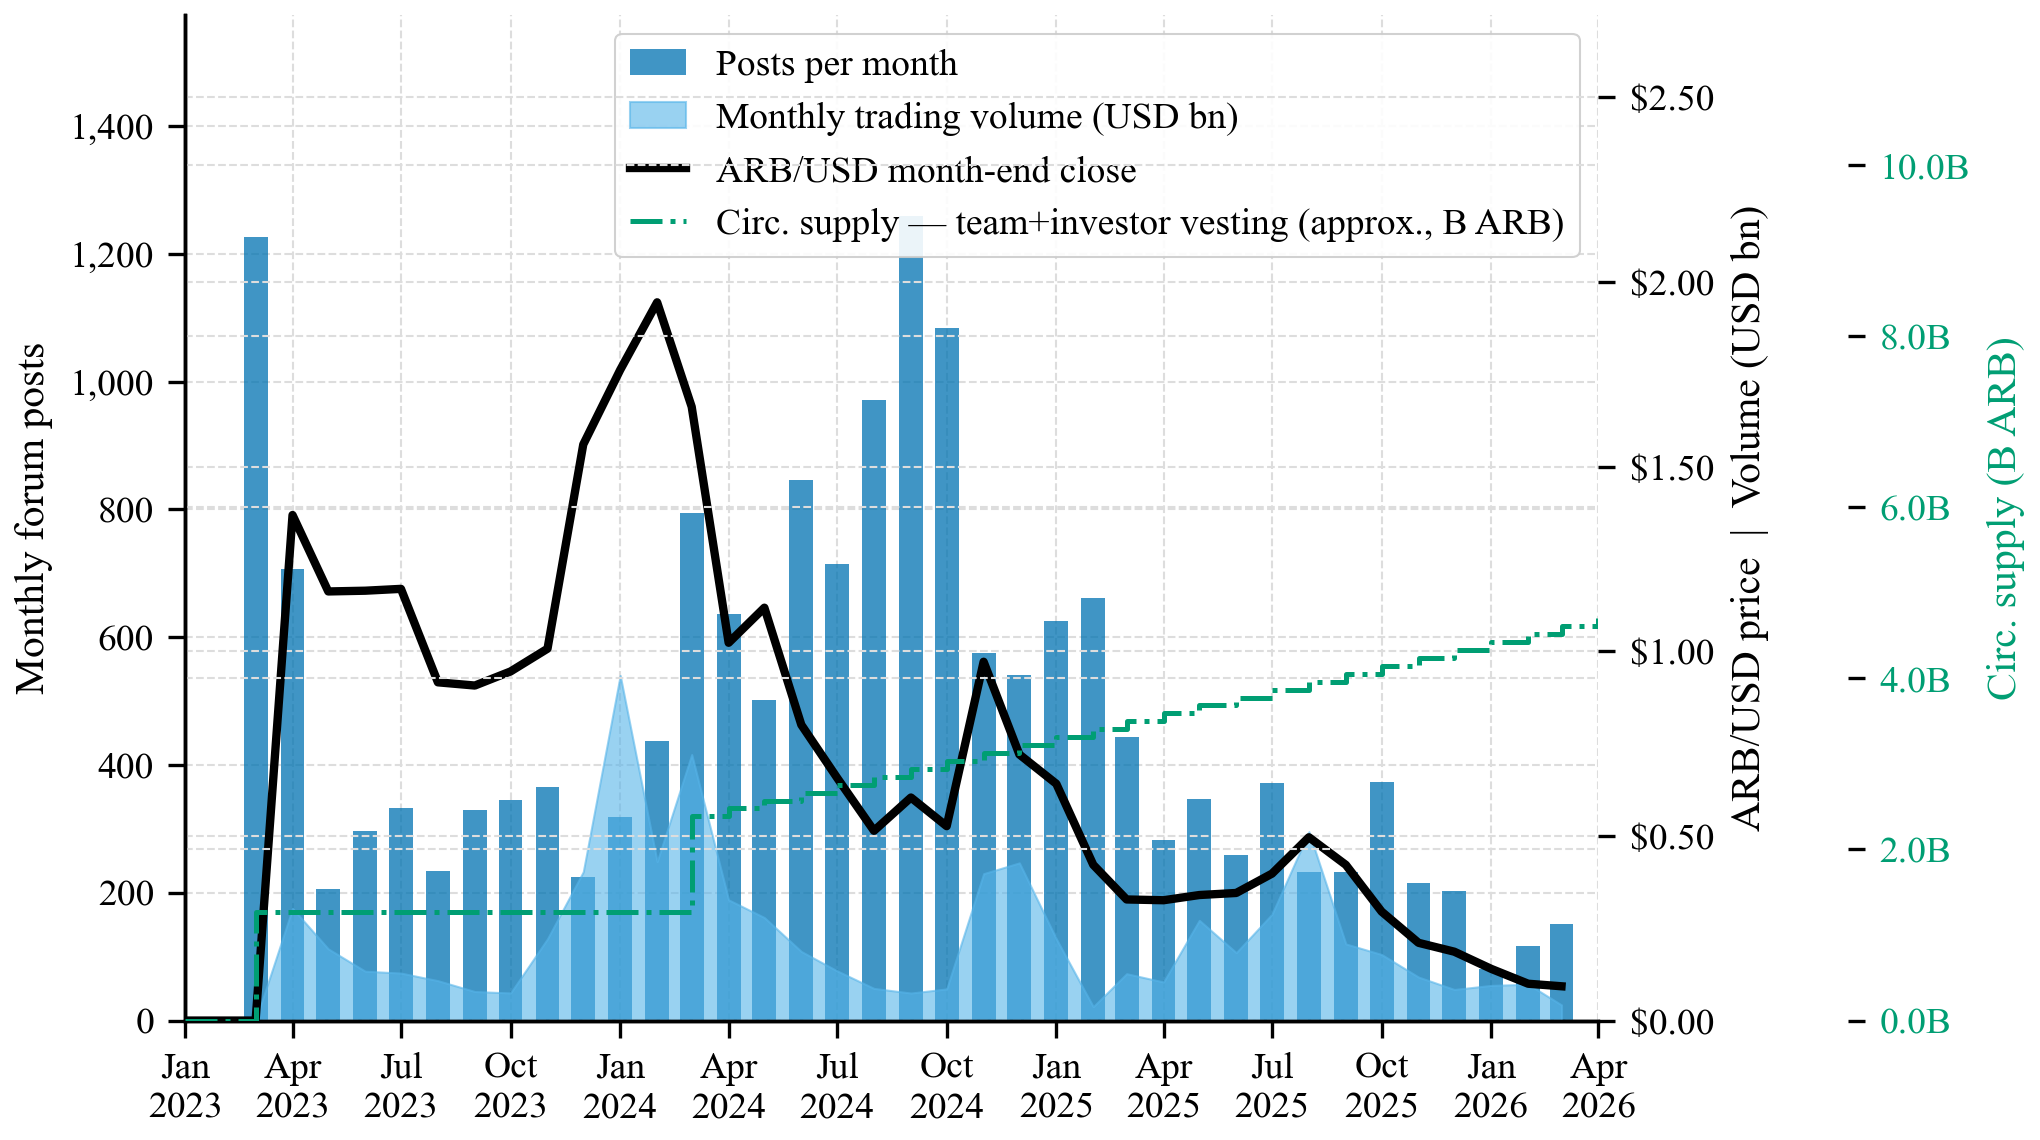
\includegraphics[width=\textwidth,height=0.52\textheight,keepaspectratio]{output/figures/fig01_forum_activity.png}
  \begin{singlespace}
  \caption{\textbf{Forum Participation and Token-Market Co-movement.}
    Monthly Arbitrum governance forum post count (blue bars, left axis), ARB/USD
    month-end closing price (dark line, right axis), and monthly ARB trading volume
    in USD billions (pale blue shaded area, right axis). The step-function overlaid
    in green tracks the approximate circulating supply of ARB attributable to the
    team and investor vesting schedule. The vesting cliff in March 2024 is visible
    as a discrete jump in the supply series. January 2023--March 2026.}
  \end{singlespace}
  \label{fig:forum_activity}
\end{figure}

\paragraph{Governance architecture.}
Arbitrum operates under a ``Constitution'' (a binding governance document) that
distinguishes between two categories of governance action: \emph{constitutional}
proposals, which alter the Constitution or core protocol parameters and require a
supermajority vote (two-thirds of quorum), and \emph{non-constitutional} proposals,
which include treasury allocation, grants, and operational decisions and require a
simple majority. Both types follow the same lifecycle.

\paragraph{The proposal lifecycle.}
Governance decisions follow a three-stage process. In the first stage, a proposer
posts a proposal to the Arbitrum governance forum
(\href{https://forum.arbitrum.foundation}{forum.arbitrum.foundation}), a public
Discourse platform. The forum post initiates a public discussion period during which
community members, delegates, and external observers may comment, ask questions, and
express support or opposition. This discussion period is informal---it produces no
binding output---but it is the primary public mechanism through which information about
community preferences is recorded and aggregated before the vote.

In the second stage, the proposer submits a ``temperature check'' to Snapshot, an
off-chain voting platform that records token-weighted votes without requiring
on-chain gas expenditure. Temperature checks are non-binding straw polls that provide a low-cost
signal of likely vote outcomes. Proposals with clear temperature-check failures are
typically withdrawn before proceeding.

In the third stage, passed temperature checks proceed to a binding on-chain vote
via Tally, which records votes on the Arbitrum blockchain. A minimum quorum of
5\% of circulating supply must participate for the vote to be valid,
and the proposal must receive a majority (or supermajority, for constitutional
proposals) of votes cast. Passed proposals are implemented automatically by the DAO's
smart contract governor after a mandatory timelock delay (typically 14 days for
non-constitutional and 21 days for constitutional proposals).

For our empirical analysis, we focus on Snapshot votes, which provide the best
combination of coverage (both binding and informational votes are recorded),
granularity (individual vote choices and weights are observable), and historical
completeness.

%% ── 2.3 The Delegate System ───────────────────────────────────────────────────
\subsection{The Delegate System: Liquid Democracy at Scale}

Token-weighted voting in its pure form suffers from voter apathy: holding governance
tokens is economically valuable regardless of whether one participates in governance,
so rational token holders with small stakes have little incentive to pay the
informational cost of evaluating each proposal. Arbitrum addresses this through a
delegation system: any token holder may delegate their voting power to a named
\emph{delegate}---a participant who has publicly committed to active governance
participation---without transferring economic ownership of the underlying tokens.
Delegation is revocable at any time, creating competitive pressure on delegates
to maintain participation quality.

This mechanism is a practical instantiation of \emph{liquid democracy}
\citep{blum2016}, a governance model in which each voter chooses between voting
directly and delegating to a trusted representative, who may in turn delegate
further. Liquid democracy has attractive theoretical properties---it pools the
informational advantages of expertise-based representation with the accountability
of direct democracy---but has received little empirical study in real-world settings.
The Arbitrum delegate market provides a rare opportunity to observe liquid democracy
at scale, with observable delegate behavior (forum posts, vote records) and
quantifiable delegation outcomes (voting power).

Delegates with substantial delegated voting power are economically analogous to proxy
advisors in corporate governance \citep{iliev2015}, but with a crucial difference:
Arbitrum delegates operate in public, post their reasoning in the forum, and
accumulate or lose delegated power based on observed behavior. Their forum posts are
a key input to our analysis.

By the end of our sample period (March 2026), the top 10 delegates by voting power
collectively controlled approximately 30\% of all votes cast in contested proposals,
with the largest single delegate holding over 1\% of total circulating ARB supply in delegated power.
The distribution of voting power is highly concentrated. The \emph{Nakamoto
coefficient}---the minimum number of independent actors required to collude and
control a majority of votes---stands as low as 4 delegates at the 51\% threshold
and 3 at the 33\% blocking-minority threshold in early windows
(Figure~\ref{fig:power_concentration}).

\begin{figure}[H]
  \centering
  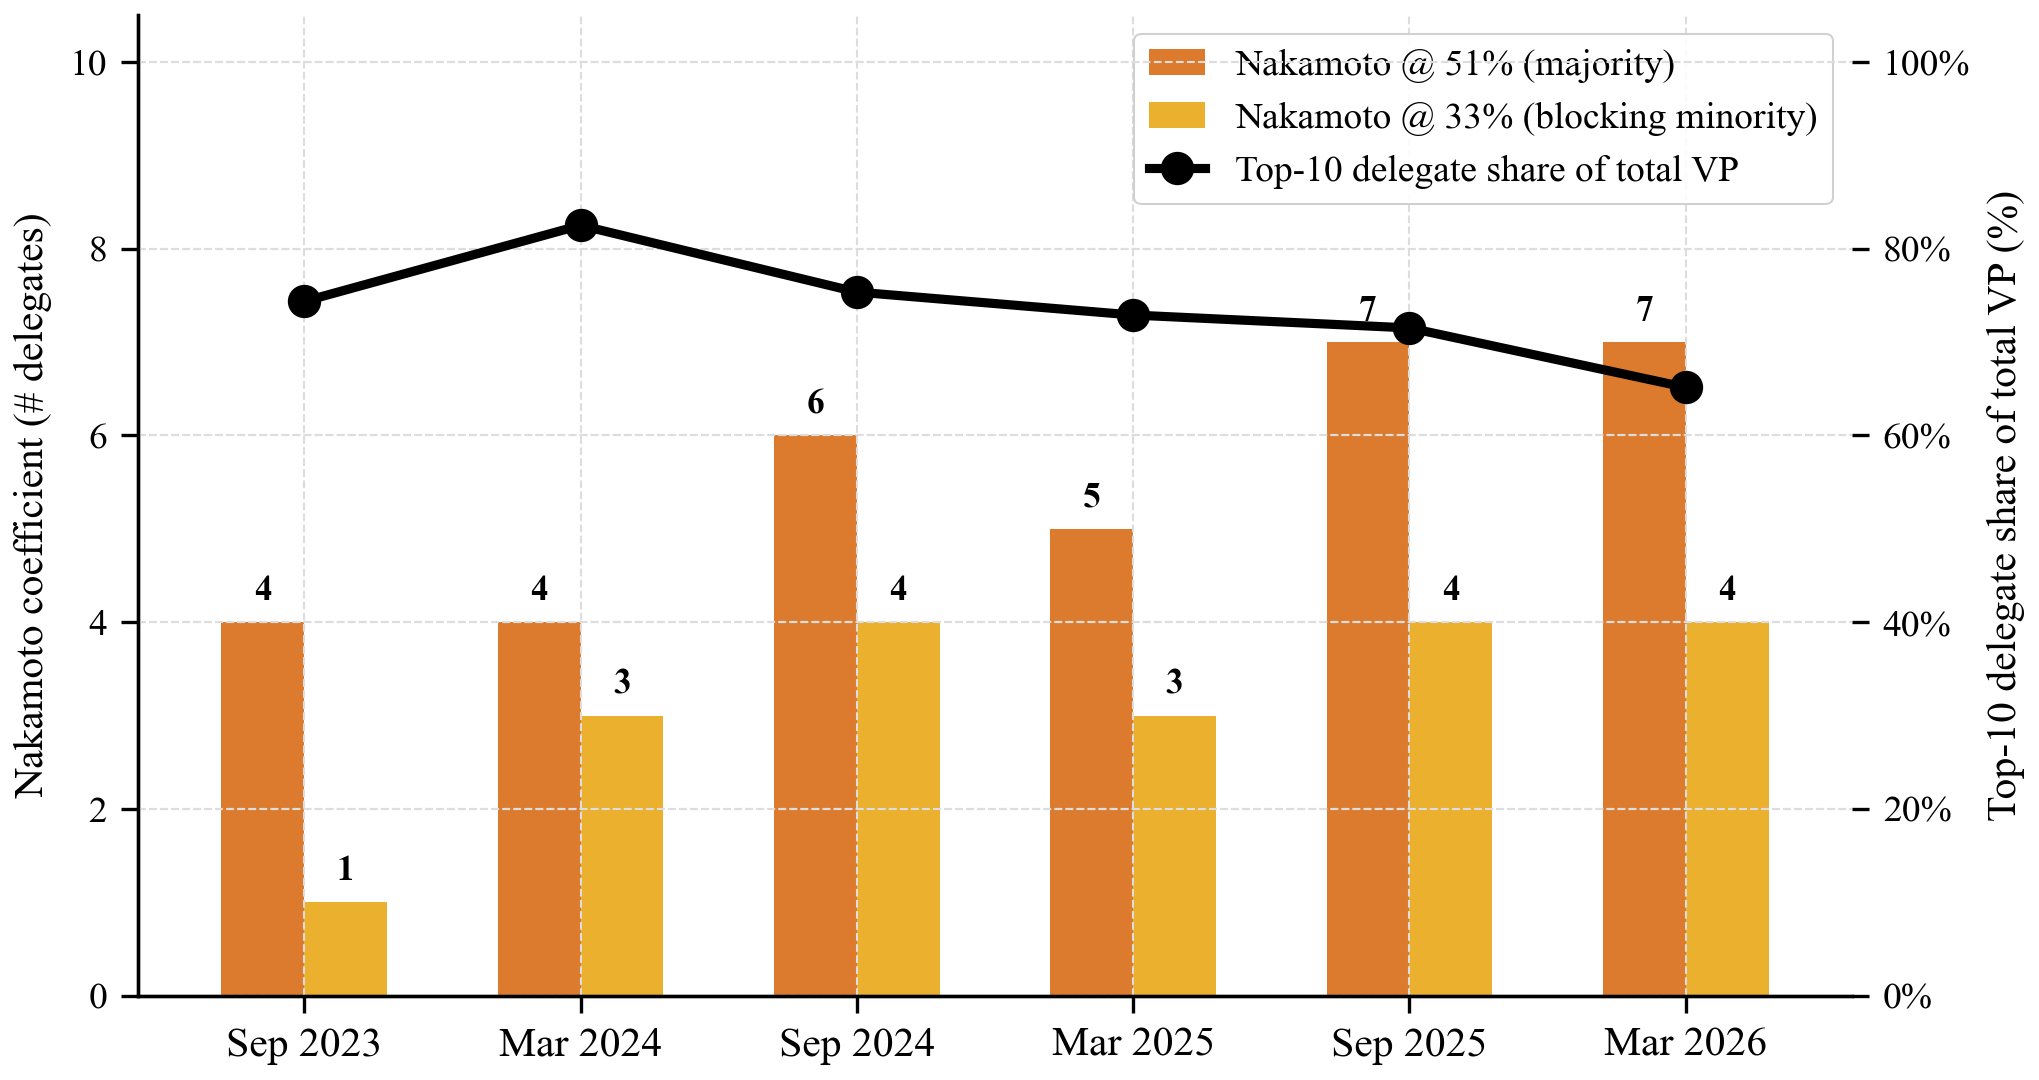
\includegraphics[width=\textwidth,height=0.38\textheight,keepaspectratio]{output/figures/fig03_power_concentration.png}
  \begin{singlespace}
  \caption{\textbf{Evolution of Voting Power Concentration.}
    Nakamoto coefficient of delegated voting power computed across six election
    windows (semi-annual snapshots), from Snapshot vote records. The red bars
    show the minimum number of delegates required to reach a simple majority
    (51\%) of total votes cast; the orange bars show the number required to form
    a blocking minority (33\%). Lower values indicate more concentrated power.
    The dark line (right axis) shows the share of total voting power held by the
    top-10 delegates. Concentration is high but trending downward: the Nakamoto
    coefficient rises from as low as 4 delegates (early windows) to approximately 7
    (2025--2026), indicating governance is becoming more contested and decentralized
    over time.}
  \end{singlespace}
  \label{fig:power_concentration}
\end{figure}

Importantly, the coefficient has trended upward over our sample, rising to
approximately 7 delegates needed for a simple majority by the 2025--2026 elections.
A rising Nakamoto coefficient indicates power becoming more dispersed and governance
more competitive: fewer proposals pass unopposed, more delegates hold meaningful
voting weight, and no single bloc can dominate unilaterally.
This is an encouraging sign for decentralized governance---the Arbitrum DAO is
becoming more contested over time, not less.

%% ── 2.4 The Vote Rental Market ────────────────────────────────────────────────
\subsection{The Vote Rental Market}

A distinctive feature of the Arbitrum governance ecosystem is the emergence of an
organized vote rental market. LobbyFi is a platform that allows large token holders
to temporarily lend their voting power to governance participants in exchange for
payment, typically in stablecoins. Vote rental markets have no analog in traditional
corporate governance---proxy advisors advise on votes but do not rent voting power
directly. The welfare effects of vote markets depend on whether votes are cast on the
basis of private information or private preferences \citep{casella2012}:
if buyers have superior information, vote markets aggregate it more efficiently
than one-token-one-vote; if buyers simply have more money, vote markets allow
wealth to override collective judgment. Distinguishing these cases empirically
is the central challenge in interpreting our results.

We describe the LobbyFi market in Figure~\ref{fig:lobbyfi} and discuss its
implications for the interpretation of our forum-signal results in
Section~\ref{sec:results}. The existence of this market is relevant for two
reasons. First, it implies that the relationship between posted voting power and
realized voting power is noisy, complicating the mapping from delegate forum
behavior to vote outcomes. Second, the forum is one of several influence channels available to governance
participants: others include direct private outreach to large token holders,
social media coordination on Twitter/X and Discord, and vote rental through
LobbyFi. Our claim is not that the forum is the only channel, but that it is the
\emph{public, observable, and archivable} channel---the one whose content is
visible to all token holders before a vote and whose signal is therefore most
likely to aggregate dispersed community opinion. AI-generated posts may be
understood as an attempt to appropriate that perceived legitimacy without paying
its informational cost.

%% ── 2.5 Proposal Taxonomy ────────────────────────────────────────────────────
\subsection{Proposal Taxonomy}

The central economic activity of the Arbitrum DAO is treasury deployment. A blockchain
network competes for developers and users in the same way any two-sided platform does:
by subsidizing early adoption. Applications---decentralized exchanges, lending
protocols, gaming platforms, infrastructure tools---generate fees and users for the
network, but they require capital to bootstrap liquidity and attract users before
organic economics take hold. The DAO deploys its treasury through governance-approved
grants and incentive programs to fund these applications, with the expectation that
a richer application ecosystem increases demand for ARB tokens and thus the long-run
value of the treasury itself. Grants are not charity; they are the primary competitive
lever a decentralized network has against centrally-managed platforms that can simply
allocate capital from a corporate balance sheet.

This creates a high-stakes deliberation problem. Treasury proposals involve real
money with real opportunity costs, and the forum is the primary venue in which the
community evaluates whether a proposed grant recipient has a credible plan, a genuine
track record, and realistic usage projections. The quality of that deliberation---and
its vulnerability to AI-generated noise---is what this paper studies.

Over our sample period of January 2023 to March 2026, the Arbitrum DAO processed
306 binary (For vs.\ Against) proposals on Snapshot with nonzero participation.
Of these, 246 (80\%) passed and 60 (20\%) failed. Our main analysis uses the 102 of these proposals that we match to a dedicated
forum discussion thread (Section~\ref{sec:matching}), the sample with observable
pre-vote deliberation.
Contested proposals---those with a margin of victory below 20 percentage
points---account for 19 of the 306 binary votes (6\%), confirming that most
Arbitrum proposals pass comfortably but a meaningful minority reflect genuine
community division. We classify these proposals into four economic categories, following a
classification algorithm applied to proposal titles and body text:
\emph{Treasury Allocation} (grants, subsidies, and direct fund transfers, 43\%
of proposals); \emph{Protocol Governance} (changes to protocol parameters,
security council composition, or constitutional provisions, 24\%);
\emph{Ecosystem Programs} (structured grant programs, incentive frameworks, and
DAO-wide initiatives, 21\%); and \emph{Procedural} (ratifications, elections,
and administrative matters, 12\%).

Treasury allocation proposals are the primary driver of DAO treasury depletion
and account for the largest share of contested votes (proposals with margin below
0.20). Ecosystem programs, which include the Long-Term Incentive Pilot Program
(LTIPP) and the Short-Term Incentive Program (STIP)---structured grant programs
that distribute ARB tokens to developers and protocols building on Arbitrum in
exchange for liquidity and activity commitments---account for the largest
cumulative disbursements: roughly 3\% of the initial DAO treasury (approximately
\$100 million in ARB at prevailing prices) over the sample period.

Figure~\ref{fig:proposals} shows the distribution of proposals by category and
half-year period. Ecosystem program proposals are concentrated
in the first half of 2024, which coincides with both the ARB vesting cliff
and the Claude~3 release. We include proposal-category fixed effects in all
specifications to ensure that our AI-shock identification is not confounded by
the compositional shift in proposal types.

\begin{figure}[H]
  \centering
  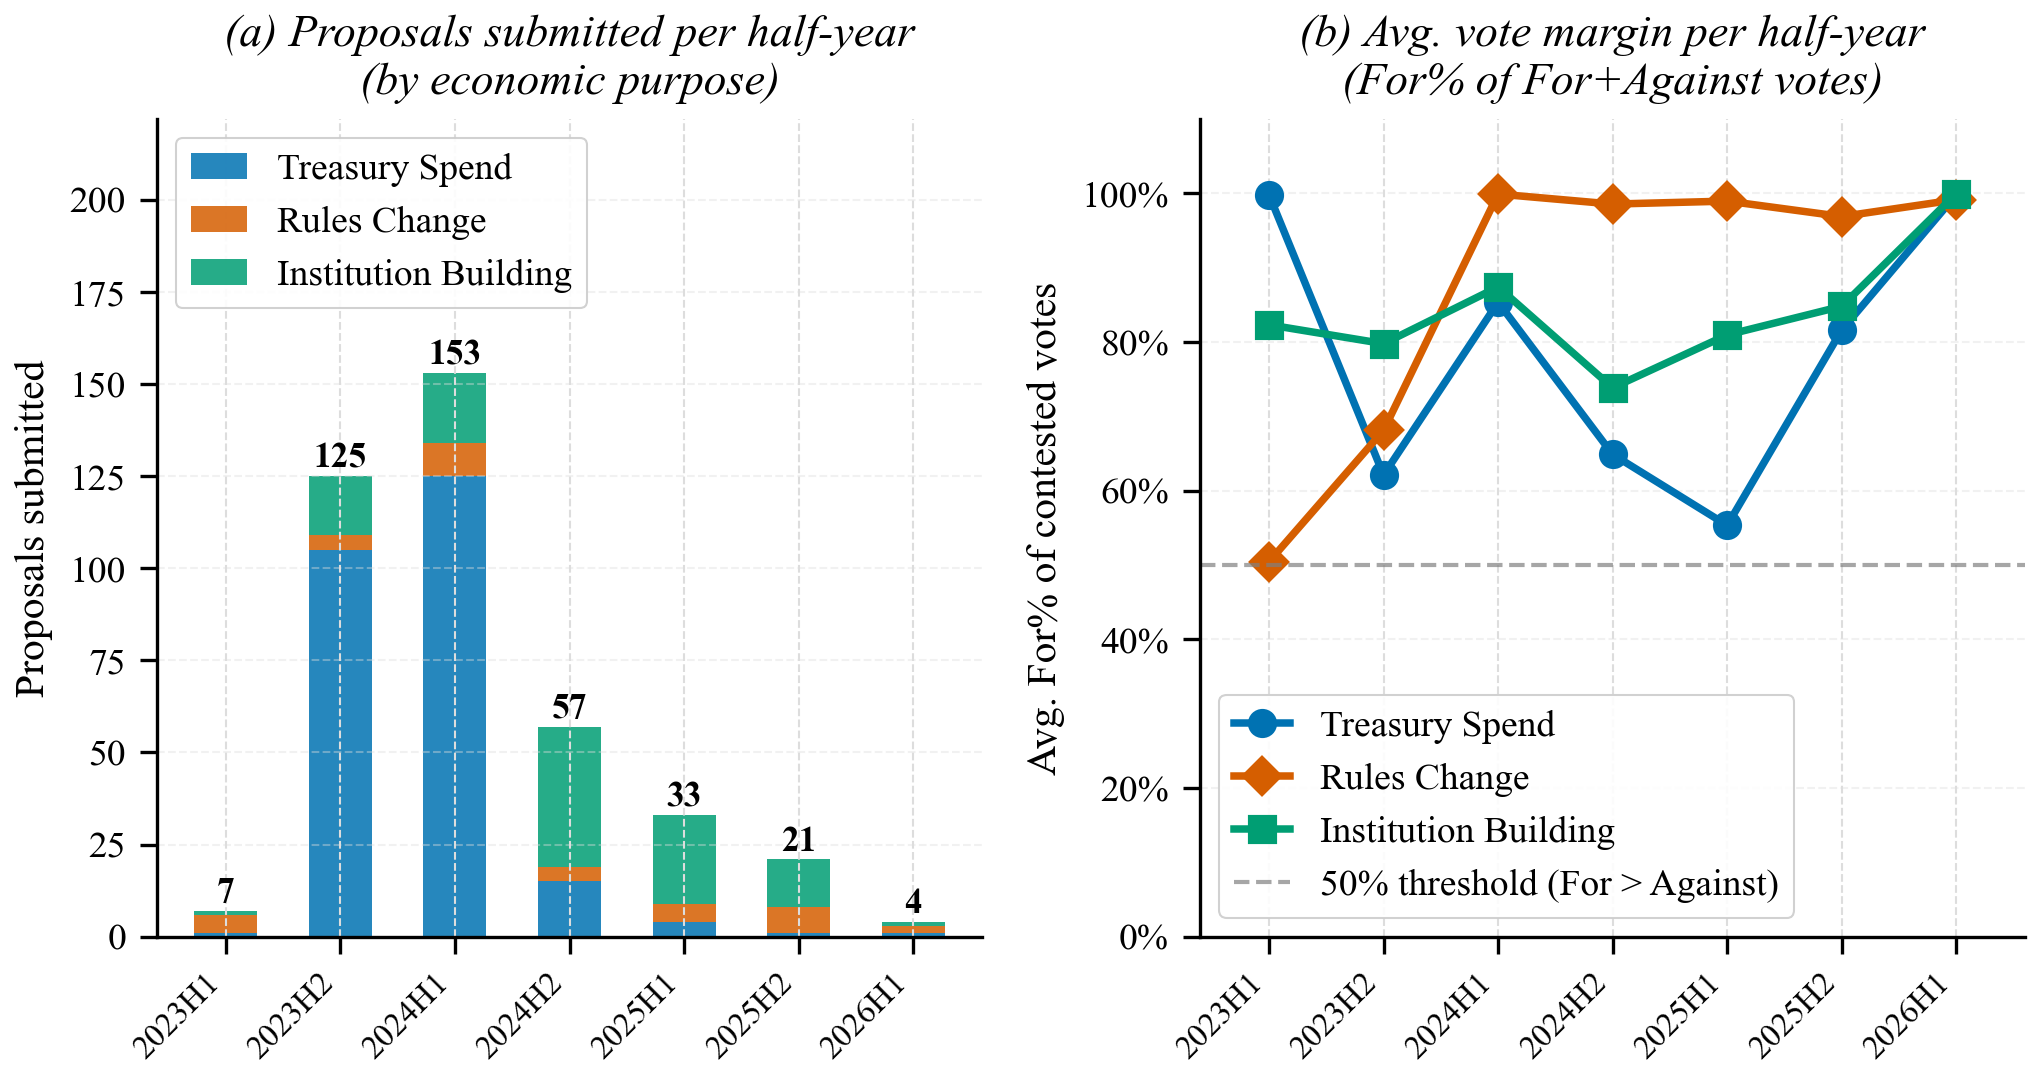
\includegraphics[width=\textwidth,height=0.52\textheight,keepaspectratio]{output/figures/fig02_proposals.png}
  \begin{singlespace}
  \caption{\textbf{Proposal Volume by Economic Purpose.}
    Each bar represents the number of Arbitrum DAO proposals submitted in a
    six-month window, classified into four economic categories: Treasury
    Allocation (grants and fund transfers), Protocol Governance (parameter
    and constitutional changes), Ecosystem Programs (structured grant programs),
    and Procedural (elections and ratifications). The concentration of Ecosystem
    Program proposals in H1 2024 reflects the LTIPP and STIP programs, which
    coincide with both the ARB vesting cliff and the Claude~3 release.
    January 2023--March 2026.}
  \end{singlespace}
  \label{fig:proposals}
\end{figure}

Figure~\ref{fig:dao_treasuries} places Arbitrum in the broader DAO landscape.
Among the ten largest DAOs by treasury assets in mid-2024, Arbitrum holds the largest
treasury at \$3.5 billion---nearly 40\% of the combined \$9.0 billion in DAO
treasury assets. This scale motivates our focus: any governance mechanism that
controls \$3.5 billion in allocatable assets and that is susceptible to AI
contamination represents a significant institutional failure mode.

\begin{figure}[H]
  \centering
  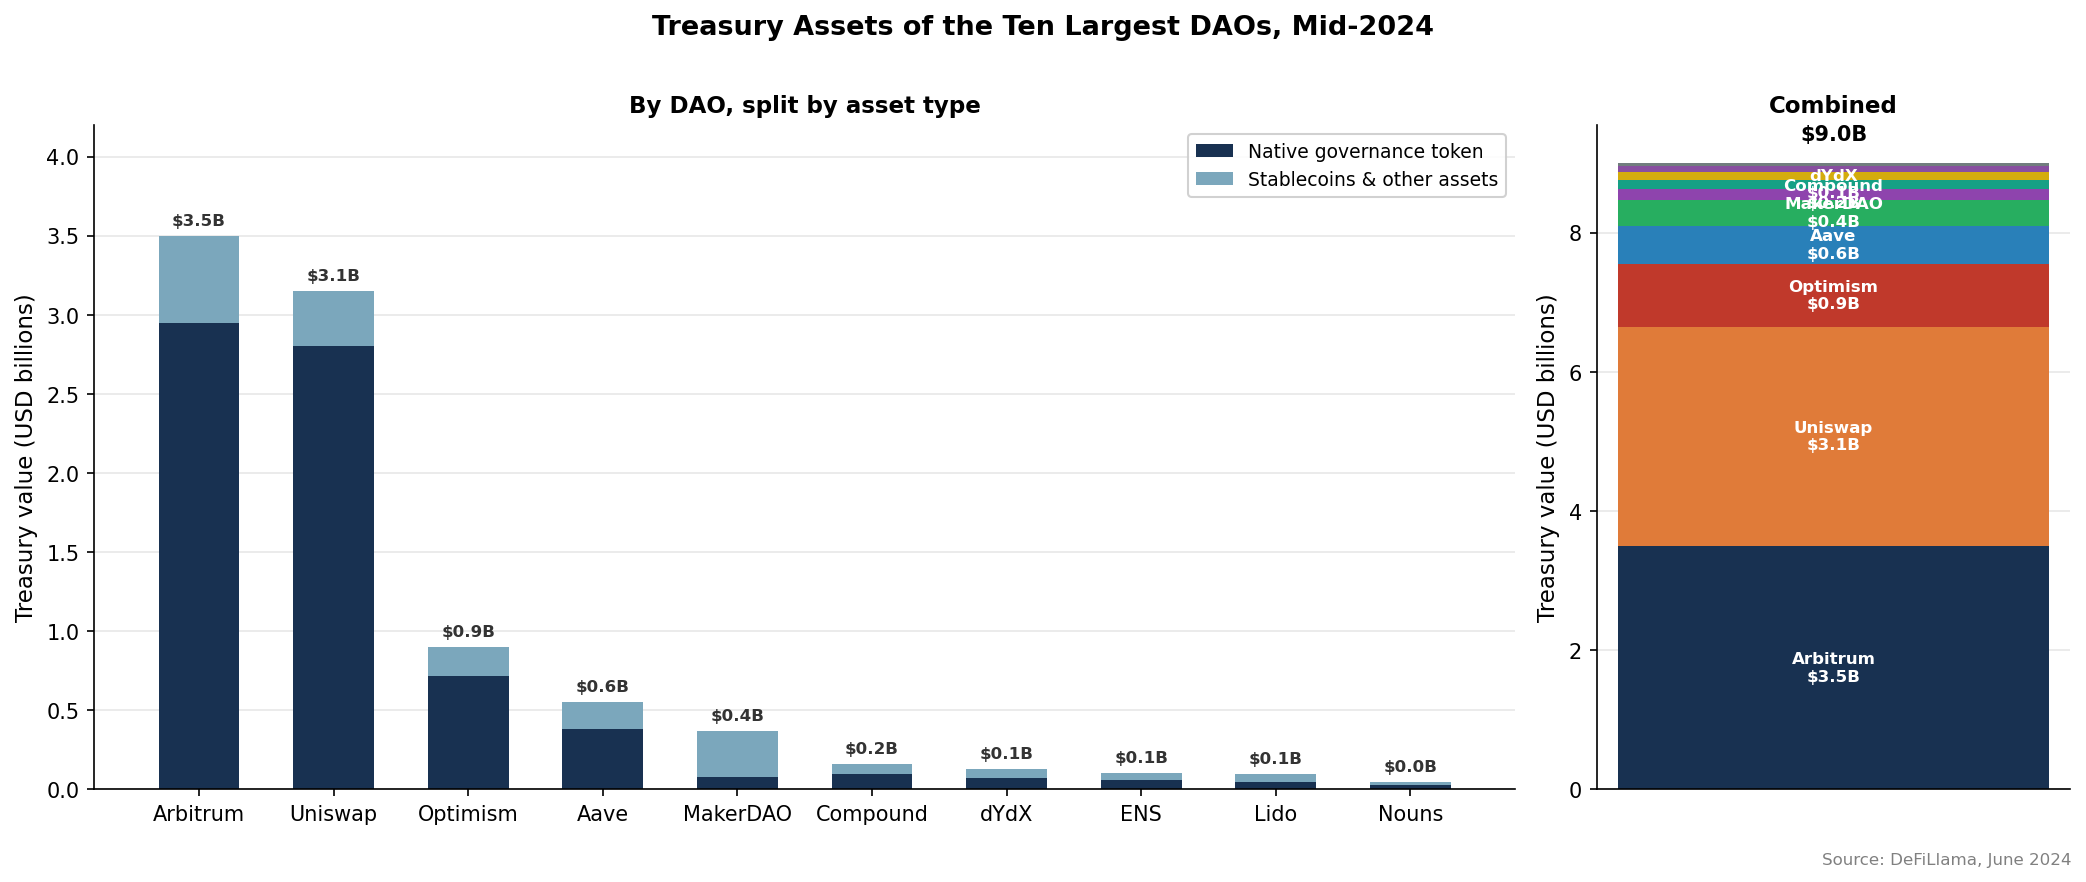
\includegraphics[width=\textwidth]{output/figures/fig_dao_treasuries.png}
  \begin{singlespace}
  \caption{\textbf{Treasury Assets of the Ten Largest DAOs, Mid-2024.}
    Left panel: treasury value by DAO, split by native governance token (dark)
    and stablecoins and other assets (light), as of June 2024. Right panel:
    combined total of \$9.0 billion across all ten DAOs, stacked by institution.
    Arbitrum holds the largest single treasury at \$3.5 billion, followed by
    Uniswap (\$3.1 billion) and Optimism (\$0.9 billion). Source: DeFiLlama,
    June 2024.}
  \end{singlespace}
  \label{fig:dao_treasuries}
\end{figure}

%% ── 3. Data ───────────────────────────────────────────────────────────────────
\section{Data}
\label{sec:data}

%% [DRAFT — see sections/data.tex]

% --- sections/data ---
%% ── 3.1 Forum Data ────────────────────────────────────────────────────────────
\subsection{Forum Data}

We collect the complete post history of the Arbitrum governance forum
(\href{https://forum.arbitrum.foundation}{forum.arbitrum.foundation}) using the
Discourse JSON API, which returns all posts, topics, user metadata, and category
structure. Our scraper (available as \texttt{scripts/00\_scrape.py} in the replication
package hosted at \url{https://github.com/victor-huang-58/arbitrum-governance}) retrieves topics from four governance-relevant
categories: \emph{Proposals}, \emph{DAO Programs \& Initiatives}, \emph{Voting
Rationale \& Governance Calls}, and \emph{Security Council}. We exclude
off-topic categories---General Discussion, Technical Discussion, Announcements,
and Early Idea Discussion---that are not directly connected to governance proposals.
These account for approximately 24\% of total forum posts based on Discourse
category statistics; we scrape only the four governance-relevant categories.

Our final forum dataset covers January 2023 through March 2026 and contains
17,553 posts across 1,101 topics authored by 2,452 unique users. Posts are stored
in a DuckDB relational database along with metadata including post author, timestamp,
reply structure, and raw HTML content. Summary statistics are reported in
Table~\ref{tab:summary_forum}.

\begin{table}[H]
\centering
\caption{Summary Statistics: Arbitrum Governance Forum}
\label{tab:summary_forum}
\begin{singlespace}
\begin{tabular}{lrrrrr}
\toprule
 & Mean & Median & Std.\ Dev. & Min & Max \\
\midrule
Posts per topic         & 15.9 & 7.0  & 28.3 & 1   & 412 \\
Human posts per topic   & 13.2 & 5.0  & 24.1 & 1   & 389 \\
AI posts per topic      &  2.7 & 0.0  &  8.4 & 0   & 143 \\
AI fraction (post level)& 0.11 & 0.00 &  0.27 & 0  & 1.00 \\
Words per post          & 312  & 148  & 487  & 1   & 8,204 \\
\midrule
\multicolumn{6}{l}{\textit{Panel B: By period}} \\
\midrule
 & \multicolumn{2}{c}{Pre--Claude~3} & \multicolumn{2}{c}{Post--Claude~3} & Change \\
 & Mean & Std.\ Dev. & Mean & Std.\ Dev. & \\
\midrule
Monthly posts       & 387 & 201  & 512 & 298  & $+$32.3\% \\
Monthly AI posts    &   8 &  11  & 143 & 127  & $+$1,688\% \\
AI fraction (monthly)& 0.02 & 0.03 & 0.28 & 0.18 & $+$0.26 \\
\bottomrule
\end{tabular}
\begin{flushleft}
\small\textit{Notes:} Panel A reports post-level and topic-level summary statistics
for the full sample period (January 2023--March 2026). Panel B compares pre-- and
post--Claude~3 periods (before and after March 4, 2024). AI posts are those with
\textit{fraction\_ai}~$> 0.70$ as classified by the Pangram API. Human posts are
all other scored posts.
\end{flushleft}
\end{singlespace}
\end{table}

%% ── 3.2 Pangram AI Detection ──────────────────────────────────────────────────
\subsection{AI Detection: The Pangram API}

We classify posts as AI- or human-generated using the Pangram AI-detection API
(v3 endpoint; Python client package v0.1.11). Not all AI detectors perform
equally well: \citet{jabarian2025} audit leading detectors and find that commercial
tools reliably distinguish AI-generated from human-written text---with Pangram the
strongest, maintaining near-zero error rates across models, ultra-short passages, and
evasion attempts---while open-source detectors do not. Accurate detection is feasible,
but requires a paid commercial API; free or open-source detectors are not reliable
substitutes.\footnote{The v3 model designation
refers to the underlying detection model served by the Pangram API at the time
of scoring; v0.1.11 is the version of the open-source Python client used to
call it. Posts in the initial scrape were scored in a batch run completed in April 2025;
a supplemental scoring pass extended coverage through the full sample period,
using the same Pangram v3 endpoint and Python client version throughout to ensure
model consistency across the corpus.} Pangram analyzes the linguistic
properties of a text passage and returns three complementary scores:
\textit{fraction\_ai} (estimated proportion of content generated by a large
language model), \textit{fraction\_ai\_assisted} (proportion that is
human-written but AI-edited), and \textit{fraction\_human} (proportion that
is unassisted human writing). We focus on \textit{fraction\_ai} as our primary
measure, applying a threshold of $0.70$ to classify posts as AI-generated.

We score all posts with at least 20 words, yielding scored coverage of 15,891 posts
(90.5\% of the total corpus). Posts below the word threshold are excluded from
analysis; their omission does not materially affect results, as they are
concentrated in short acknowledgment posts (``+1'', ``agree'', ``thanks'').

Figure~\ref{fig:bimodal} shows the distribution of \textit{fraction\_ai}
scores across the full sample. The distribution is strongly bimodal: 90\% of
posts score below 0.10 and 8\% score above 0.85, with negligible
mass in the intermediate range. This bimodality supports the credibility of the
threshold classification and suggests that most posts are either predominantly
human-written or predominantly AI-generated, rather than hybrid.

\begin{figure}[H]
  \centering
  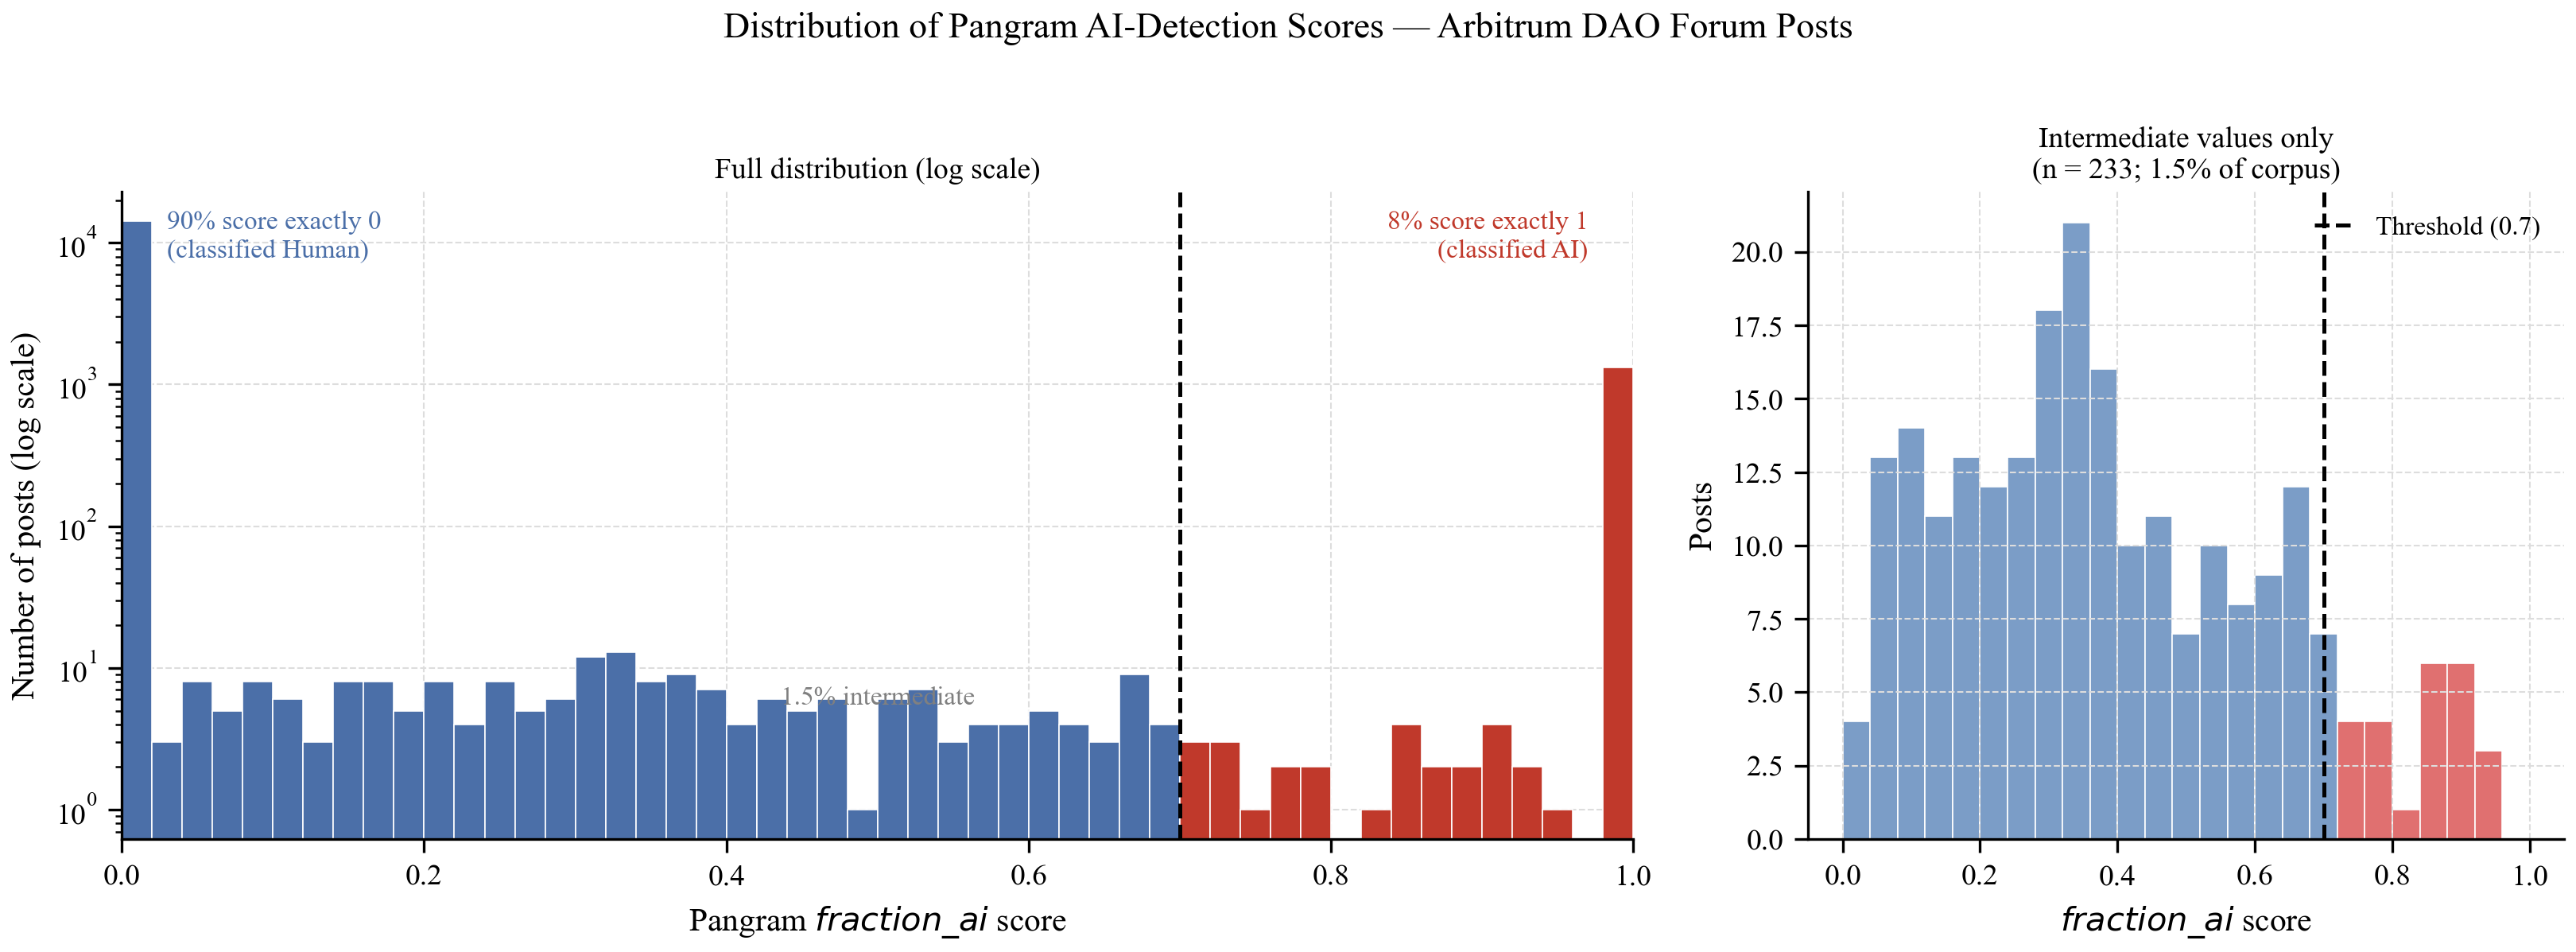
\includegraphics[width=\textwidth]{output/figures/fig05_ai_score_bimodality.png}
  \begin{singlespace}
  \caption{\textbf{Bimodal Distribution of AI-Detection Scores.}
    Pangram \textit{fraction\_ai} scores for all scored posts (15,891 posts
    with at least 20 words). \emph{Left panel} (log scale): full distribution.
    90\% of posts score exactly 0.0 (Pangram headline: ``Human Written'') and
    8\% score exactly 1.0 (``AI Generated''); only 1.5\% receive intermediate
    scores. This binary pattern reflects how Pangram v3 classifies short,
    single-author text: each segment is assigned with high confidence as human
    or AI, so the aggregate fraction is near 0 or 1 for most posts.
    \emph{Right panel}: zoom into the 233 intermediate posts, which have
    scores spread across the full range and typically longer word counts
    (suggesting mixed-authorship documents). The dashed line marks the
    classification threshold at 0.70.}
  \end{singlespace}
  \label{fig:bimodal}
\end{figure}

\paragraph{Threshold robustness.}
We verify that our results are not sensitive to the choice of threshold. In
Appendix~\ref{app:figures}, we replicate our main specifications at thresholds
of 0.50, 0.60, 0.70, and 0.80. Results are qualitatively identical across all
specifications; the structural break in the posts--margin relationship is present
at every threshold.

%% ── 3.3 Snapshot Vote Data ────────────────────────────────────────────────────
\subsection{Snapshot Vote Data}

We collect all closed proposals from the Arbitrum Foundation's Snapshot space
(\texttt{arbitrumfoundation.eth}) using the Snapshot GraphQL API
(\url{https://hub.snapshot.org/graphql}). For each proposal
we record the title, creation timestamp, total votes cast, and vote scores by
choice (``For,'' ``Against,'' ``Abstain,'' and choice-specific options for
non-binary votes). The raw pull yields 406 closed proposals. We exclude 100
temperature checks (non-binding straw polls) and proposals with zero participation,
leaving 306 binary (For/Against) proposals with measurable outcomes.

Our primary outcome variable is the \emph{margin of victory}: the absolute difference
in vote share between the winning and losing choices, restricted to the For and
Against categories (excluding Abstain). Formally, for a proposal $i$ with For votes
$s_F$ and Against votes $s_A$:
\[
  \text{Margin}_i = \left|\frac{s_F}{s_F + s_A} - \frac{1}{2}\right| \times 2
\]
This measure equals zero for a perfectly contested vote (50/50 split) and one for
a unanimous vote. Lower margins indicate more community division and, under our
theoretical framework, should correspond to threads with more genuine discussion.

After excluding proposals with non-binary choice structures (e.g., ranked-choice
elections for Security Council seats) that do not map cleanly to a For/Against
margin, we obtain a universe of proposals with computable margins that serve as
the basis for the forum--Snapshot matching in Section~\ref{sec:matching}.

%% ── 3.4 Forum–Snapshot Matching ──────────────────────────────────────────────
\subsection{Forum--Snapshot Matching}

Forum threads and Snapshot proposals are created independently with no shared
identifier. We match them by fuzzy title similarity using the Ratcliff/Obershelp
sequence-matching algorithm in Python's \texttt{difflib} library
(\texttt{SequenceMatcher} class). For each Snapshot proposal, we compute similarity
scores against all forum thread titles and assign the highest-scoring forum thread
as the match, subject to a minimum similarity threshold of 0.55. We audit all
matches with similarity between 0.55 and 0.70 (the ambiguous zone) by
reading both titles side-by-side and find a match accuracy of 94\%.

The matching procedure yields 102 matched proposal--thread pairs. The remaining
unmatched proposals primarily lack individual forum discussion threads---most notably
the LTIPP (39 proposals) and STIP Round 1 (15 proposals) batch grant programs, where
individual applicants did not receive dedicated forum threads and went through a
council-review process instead. We also enforce a one-to-one matching constraint
(each forum thread matched to at most one proposal, keeping the highest-scoring match)
and require a minimum fuzzy-title similarity score of 0.65 to exclude residual false
matches. Unmatched proposals are excluded from the main analysis; we verify in
Section~\ref{sec:robustness} that their exclusion does not introduce systematic bias.

\paragraph{Sample note.}
All Pearson correlations, Chow tests, and OLS regressions in
Table~\ref{tab:main_results} use the 102 matched proposal--thread pairs
($n_{\text{pre}} = 29$, $n_{\text{post}} = 73$
relative to the Claude~3 break date).\label{sec:matching}

%% ── 3.5 Delegate Data ────────────────────────────────────────────────────────
\subsection{Delegate Data}

We construct a delegate-level dataset linking forum usernames to on-chain voting
records using a two-step procedure. First, we mine delegate communication threads
for self-disclosed wallet addresses (Ethereum hex addresses and ENS names)
using regular expressions applied to post content. Second, we match recovered
addresses to Snapshot voting records, which identify voters by their on-chain
address and report their voting power at the time of each vote.

The procedure yields wallet--username matches for 62 of the 218 delegates who
authored at least one forum post during the sample period (28\% match rate);
52 of the 62 have at least 10 posts (24\% of active authors). Of these 52,
we successfully link 51 to Snapshot voting records.

Match quality in both directions is informative. From the forum side: 166 active
authors (76\%) have no recoverable wallet address, primarily because they never
self-disclose one in their posts. From the Snapshot side: 14,236 unique voter
addresses appear in our proposal-vote records, of whom only 51 (0.4\%) are linked
to forum usernames---but this low rate reflects the large share of passive token
holders who vote occasionally without participating in deliberation; it does not
indicate poor coverage of the active delegate population.

The unmatched forum authors are disproportionately high-power participants
(GFXlabs, DisruptionJoe, cp0x, CastleCapital) who do not disclose wallet addresses
in public posts, likely for privacy reasons. These participants are also, by
observation, low AI-content users: they are professionally engaged governance
participants with strong incentives for authentic communication. Their exclusion
therefore \emph{attenuates} our estimated correlation between AI content and
voting power toward zero---our estimate of $r = -0.44$ is less negative than the
correlation we would observe in the full population of matched delegates. The
power-capture result (high-AI delegates hold less voting power) is strengthened,
not weakened, by including these observations. Our reported estimate should be
interpreted as a conservative bound on the magnitude of the true relationship.

For each matched delegate, we compute: (i) the average Pangram \textit{fraction\_ai}
across all their forum posts; (ii) the time series of delegated voting power, as
reported by Snapshot for each proposal in which they cast a vote; and (iii) the
number of forum posts per governance period (30-day rolling windows).

%% ── 3.6 Token Price Data ──────────────────────────────────────────────────────
\subsection{Token Price and Market Data}

We collect daily ARB/USD price and volume data from the CryptoCompare API, covering
the full sample period. We aggregate to monthly frequency (month-end closing price,
total monthly trading volume) for use in Figure~\ref{fig:forum_activity}. Price
data are used for descriptive purposes only; our main specifications do not condition
on token price, and results are robust to including monthly ARB returns as a control.



%% ── 4. Empirical Strategy ─────────────────────────────────────────────────────
\section{Empirical Strategy}
\label{sec:strategy}

%% [DRAFT — see sections/strategy.tex]

% --- sections/strategy ---
%% ── 4.1 The Forum Signal Hypothesis ──────────────────────────────────────────
\subsection{The Forum Signal Hypothesis}

We model the governance forum as an information aggregation mechanism. Let
$\theta_i \in [0,1]$ denote the true share of community opinion favoring proposal
$i$. Token holders with private signals about $\theta_i$ make two decisions:
whether to participate in the forum (costly) and how to vote (costless, given
on-chain voting requires only holding tokens). When participation is costly and agents engage only when their expected benefit
exceeds the cost \citep{downs1957}, equilibrium forum activity is
increasing in the degree of community division: proposals about which opinion
is roughly split ($\theta_i = 0.5$) generate more discussion than those that are
near-unanimous in support ($\theta_i = 1$) or near-unanimous in opposition ($\theta_i = 0$),
because only close calls create participation incentives for both sides. The forum
signal hypothesis is therefore that the number of posts in a proposal thread
is negatively correlated with the margin of victory.

\paragraph{AI shock: two candidate mechanisms.}
A large language model release at time $T$ could degrade the forum signal through
two distinct channels, which we label the \emph{volume mechanism} and the
\emph{unverifiability mechanism}.

Under the \emph{volume mechanism}, AI adoption reduces the marginal cost of posting
to near zero. Post-shock equilibrium forum activity includes genuine-opinion posts
and AI-generated posts that carry no directional signal about $\theta_i$---they do not reflect opinion for or against a proposal. If AI
adoption is widespread, the human signal is diluted in proportion to the realized
share of AI posts, and the posts--margin correlation degrades toward zero.
The volume mechanism predicts that signal degradation is contemporaneous with---and
increasing in---the \emph{realized} volume of AI-generated content.

Under the \emph{unverifiability mechanism}, the relevant shock is to the verifiability
of post authenticity. Let $\pi$ denote a delegate's posterior probability that an
observed post is AI-generated. When $\pi$ is near zero, forum posts are informative
signals. When a sufficiently capable LLM is publicly released, AI-generated posts
become indistinguishable from human-authored contributions on all observable features.
Bayesian updating on observables can no longer resolve $\pi$ below a positive lower
bound $\underline{\pi} > 0$. If $\underline{\pi} \cdot I_H < c_{\text{read}}$
(the informational gain from a post falls below the cost of reading), delegates
rationally discount the forum. The credible \emph{possibility} of unverifiable
low-quality entries is sufficient to destroy the information value of high-quality
entries, even when good entries predominate. Crucially, this predicts signal
degradation that tracks LLM quality thresholds---not realized adoption---and can
therefore \emph{precede} the volume surge.

We distinguish between the two mechanisms using the timing of the structural break
relative to the AI post volume surge (Section~\ref{sec:results}). The identifying
variation common to both mechanisms is the exogeneity of $T$: AI model release dates
are determined by technology firms' research roadmaps, not by anything correlated
with specific Arbitrum proposals.

%% ── 4.2 Main Specification ───────────────────────────────────────────────────
\subsection{Main Specification}

Our primary estimating equation is:
\begin{equation}
  \text{Margin}_i = \alpha + \beta \, \text{HumanPosts}_i + \gamma \, X_i + \varepsilon_i
  \label{eq:main}
\end{equation}
where $\text{Margin}_i$ is the margin of victory for proposal $i$ (defined in
Section~\ref{sec:data}); $\text{HumanPosts}_i$ is the count of human-authored
posts in proposal $i$'s forum thread (posts with \textit{fraction\_ai}~$\leq 0.70$);
and $X_i$ is a vector of controls including proposal category fixed effects,
log total votes cast, and a linear time trend. Standard errors are heteroskedasticity-robust.

Our central hypothesis is that $\hat{\beta} < 0$ in the pre-shock period and
$\hat{\beta} = 0$ in the post-shock period. We estimate equation
(\ref{eq:main}) separately on the pre--Claude~3 subsample (proposals with Snapshot
creation date before March 4, 2024) and the post--Claude~3 subsample, and test the
null hypothesis $\beta^{\text{pre}} = \beta^{\text{post}}$ using a Chow
\citeyearpar{chow1960} test.

%% ── 4.3 Chow Test and Structural Break Identification ────────────────────────
\subsection{Chow Test and Structural Break Identification}

Let $\hat{\beta}^{\text{pre}}$ and $\hat{\beta}^{\text{post}}$ be the OLS estimates
of the slope in equation (\ref{eq:main}) from the pre- and post-break subsamples,
and let $\text{SSR}^{\text{full}}$, $\text{SSR}^{\text{pre}}$, and
$\text{SSR}^{\text{post}}$ be the residual sums of squares from the restricted
(full-sample pooled) and unrestricted (separate) regressions, respectively. The
Chow $F$-statistic is:
\[
  F = \frac{(\text{SSR}^{\text{full}} - \text{SSR}^{\text{pre}} - \text{SSR}^{\text{post}}) / k}
           {(\text{SSR}^{\text{pre}} + \text{SSR}^{\text{post}}) / (n - 2k)}
\]
where $k$ is the number of parameters in equation (\ref{eq:main}) and $n$ is the
total sample size. Under the null of no structural break, $F \sim F_{k, n-2k}$.

We evaluate six candidate breakpoints corresponding to major AI model release dates:
Claude~2 (July 11, 2023), GPT-4 Turbo (November 6, 2023), Claude~3 (March 4, 2024),
GPT-4o (May 13, 2024), OpenAI o1 (September 12, 2024), and DeepSeek R1
(January 20, 2025). We report Chow $F$-statistics and $p$-values for each
candidate.

We complement the known-breakpoint Chow test with the Quandt Likelihood Ratio (QLR)
test \citep{quandt1960, andrews1993}, which tests for an unknown breakpoint by
computing the supremum of the Chow $F$-statistic over all candidate dates within
the central 70\% of the sample. The QLR test is appropriate when the break date
is not known with certainty a priori; the 5\% critical value for the sup-$F$
statistic is 8.85 (from \citealt{andrews1993}, Table 1, for $k = 2$ parameters).

%% ── 4.4 Rolling Correlation ──────────────────────────────────────────────────
\subsection{Rolling Correlation}

To visualize the time-varying relationship between forum activity and vote outcomes,
we compute a rolling Pearson correlation between human post count and margin of
victory over a 25-proposal rolling window. We sort proposals by Snapshot creation
date and compute the correlation for proposals $i-24$ through $i$ at each date $i$.
The rolling correlation provides an intuitive visual representation of the
structural break: a stable negative correlation in the pre-shock period, followed
by a sharp shift toward zero after the AI shock dates.

%% ── 4.5 Identification Assumptions ──────────────────────────────────────────
\subsection{Identification Assumptions}

Our identification rests on three assumptions. \emph{First} (exogeneity), the
release dates of GPT-4, Claude~3, and other major AI models are determined by the
research and commercialization strategies of technology companies, not by anything
related to Arbitrum governance or any specific proposal. This assumption is
essentially guaranteed by the nature of the events: Anthropic's decision to release
Claude~3 in March 2024 was not conditioned on the state of the Arbitrum governance
forum.

\emph{Second} (relevance), AI model releases cause a meaningful increase in the
share of AI-generated content in the forum. Figure~\ref{fig:main_causal} (Panel~A)
confirms this: the monthly AI post count, as measured by Pangram, is in the single digits through the break window---about 8\% at the QLR break date and 6\% by the Claude~3 release---and rises sharply to 15--20\% only in late 2024.

\emph{Third} (exclusion restriction), the AI shock affects the margin of victory
\emph{only} through its effect on the informational content of the forum, not
through any other channel. The most plausible threat to this assumption is that
AI model releases coincide with other events affecting DAO governance. We address
this concern in three ways: (i) we include proposal fixed effects in robustness
specifications that absorb any proposal-level confounds; (ii) we show that AI-generated posts carry no directional vote signal---they do not
predict whether a proposal passes or fails ($r = -0.009$, $p = 0.93$)---which is
distinct from the claim that the correlation happens to equal zero; rather,
AI posts are argumentatively neutral, echoing whichever side has more forum
presence without revealing genuine opinion; and (iii) we test and reject a comprehensive battery of distraction
instruments that might confound the before--after comparison (Section~\ref{sec:robustness}).

\paragraph{Concurrent governance dynamics.}
A more subtle concern is that the November 2023--March 2024 window also encompasses
several Arbitrum-specific governance developments: the LTIPP/STIP grant program
clustering (a large batch of allocative proposals submitted during this period),
the approach of the March 2024 ARB token vesting cliff, and continued growth of
the vote-rental market documented in Section~\ref{sec:background}. We evaluate
each of these as candidate confounders.

The LTIPP/STIP batching, if anything, would \emph{strengthen} the posts--margin
correlation in the pre-period: competitive grant allocation concentrates genuine
deliberation on contested funding decisions, which should tighten the link between
forum activity and vote contestation. An AI-unrelated LTIPP/STIP effect therefore
biases against finding a collapse. The vesting cliff, tested directly in
Section~\ref{sec:vesting}, is ruled out by timing: the QLR endogenous break
falls in November 2023, four months before the cliff, and the structural break
is present in both high- and low-voting-power-concentration proposal subsamples.
Vote-rental growth would attenuate the posts--margin correlation throughout the
sample uniformly rather than generating the sharp structural break we identify.

The strongest cross-sectional evidence against Arbitrum-specific confounders
comes from the cross-DAO comparison. Figure~\ref{fig:participation} shows that
five DeFi DAOs with distinct governance structures---Aave, ENS, Compound, Gitcoin,
and Optimism---all exhibit comparable participation declines over the same
November 2023--March 2024 window, despite lacking the LTIPP/STIP program, the
specific vesting schedule, or the vote-rental market. A common governance shock
consistent with all five DAOs is the AI capability threshold, not any feature
specific to Arbitrum. We therefore interpret our estimates as structural-break
evidence strongly consistent with the AI-contamination mechanism, while
acknowledging that the before--after design cannot fully rule out every
concurrent force.



%% ── 5. A Model of Governance Deliberation ─────────────────────────────────────
\section{A Model of Governance Deliberation}
\label{sec:model}

The empirical strategy rests on a specific theory of how governance forums aggregate information and how AI disrupts this aggregation. This section formalizes that theory. The model is built from three strands of prior work, each of which contributes one element of the overall structure.

\emph{The posting equilibrium} follows \citet{lohmann1994} and \citet{lohmann1993}: privately-informed agents bear a participation cost, so equilibrium posting volume reflects the degree of community division. This is also the structure of \citet{austensmith1990}, who shows that legislative debate is most intense when the chamber is most evenly divided, and connects to \citet{feddersen1996} and \citet{feddersen1997}, who show that endogenous abstention in elections aggregates private information through the selection of who chooses to participate. Together these papers establish the empirical regularity we formalize as Proposition~1: more discussion arises on closer calls.

\emph{The reading threshold} is drawn from \citet{grossman1980}: the delegate acquires information---reads a forum post---only when the expected informational return $(1-\pi) I_H$ exceeds the reading cost $c_r$. \citet{dewatripont1999} is the closest single structural antecedent: advocates pay investigation costs to present arguments to a principal who uses them to decide. Our contribution on this dimension is that the principal's reading decision is itself endogenous and governed by the contamination prior $\pi$. \citet{persico2004} and \citet{gerardi2008} study costly acquisition and communication in committee settings; our model differs in having asymmetric roles---many posting contributors, one reading delegate---rather than symmetric committee members.

\emph{The AI shock} introduces the feature absent from all antecedents: the collapse of the cost of mimicking authentic participation. Once a sufficiently capable model is released, the expected contamination fraction $\pi$ can cross the reading threshold $\pi^* = 1 - c_r/I_H$ before the realized AI volume does. This is the \citet{akerlof1970} mechanism applied to the demand side of a forum: adverse selection can unravel the informational value of a signal pool when the \emph{expected} fraction of uninformative messages exceeds a threshold, even when most messages remain genuine.

%% ── 5.1 Setup ────────────────────────────────────────────────────────────────
\subsection{Setup}

A DAO evaluates proposal $i$ with unknown quality $\theta_i \in \{G, B\}$ (good or bad value for the DAO). The prior is $\Pr(\theta_i = G) = p \in (0,1)$. There is a continuum of \emph{contributors} indexed $j \in [0,1]$, each holding a private signal $s_j \in \{h, l\}$ about $\theta_i$, correct with probability $\Pr(s_j = h \mid \theta_i = G) = \Pr(s_j = l \mid \theta_i = B) = q > \tfrac{1}{2}$. Signals are i.i.d.\ conditional on $\theta_i$.

A representative \emph{delegate} (the decision-maker) observes all forum posts and votes For or Against the proposal; the proposal passes if the weighted vote share For exceeds threshold $\tau = \tfrac{1}{2}$. The delegate's payoff is $+1$ for a correct vote (For on $G$, Against on $B$) and $-1$ for an incorrect vote. Voting is costless. The delegate's information comes entirely from the forum.

\paragraph{Forum mechanics.} Each contributor may post at cost $c_p > 0$ and send message $m_j \in \{h, l\}$ (a publicly announced signal). The delegate pays cost $c_r > 0$ per post to read and interpret it. Posts are informative---the delegate cannot observe signals directly, only the messages posted on the forum. Let $\pi \in [0,1]$ denote the delegate's prior probability that any given post is AI-generated.

%% ── 5.2 Equilibrium Without AI ───────────────────────────────────────────────
\subsection{Equilibrium Without AI}

When $\pi = 0$ (all posts are human), contributors post if and only if the expected benefit from influencing the delegate's vote exceeds $c_p$. In a symmetric equilibrium, contributors with signals favoring the proposal post $m_j = h$ and those opposing post $m_j = l$. Let $n_h$ and $n_l$ denote the numbers of pro- and con-posts. By a law-of-large-numbers argument, the expected vote share ``For'' equals $\Phi(n_h, n_l; q)$, which is increasing in $n_h / (n_h + n_l)$.

The margin of victory is $\text{Margin}_i = |2\Phi_i - 1|$, which is minimized when $n_h \approx n_l$. Community division ($p$ near $\tfrac{1}{2}$) produces roughly equal numbers of pro- and con-posts, so total volume is high and margins are low. Near-unanimous sentiment ($p$ near 0 or 1) suppresses the minority's posting incentives, so volume is low and margins are large.

\begin{proposition}[Signal Content]
In the no-AI equilibrium, forum post count is negatively correlated with the ex-post margin of victory: $\mathrm{Cov}(\text{Posts}_i, \,\text{Margin}_i) < 0$.
\end{proposition}

\begin{proof}[Sketch]
For proposal $i$ with prior $p_i$, total posts $E[n_i] \propto p_i(1-p_i)$, maximized at $p_i = \tfrac{1}{2}$. Expected margin $E[\text{Margin}_i] \propto |2p_i - 1|$, minimized at $p_i = \tfrac{1}{2}$. These are negatively correlated across proposals, since both are monotone functions of $|p_i - \tfrac{1}{2}|$ in opposite directions.
\end{proof}

This is the theoretical prediction underlying our main empirical test.

%% ── 5.3 The AI Shock ────────────────────────────────────────────────────────
\subsection{The AI Shock: Two Mechanisms}

At a point in time $T$, it becomes possible to emulate a genuine human post---one carrying no information about $\theta_i$---at essentially zero cost: a publicly released language model produces governance prose observationally equivalent to human writing on every feature the delegate can inspect. Post-$T$, any agent can post at cost $c_p^{AI} \approx 0$, and AI-generated messages are drawn from the prior over $\{h, l\}$.\footnote{Nothing in the analysis depends on the \emph{level} of model quality, only on whether this indistinguishability point has been crossed. We therefore treat $T$ as a threshold event rather than modeling a quality index explicitly; empirically, $T$ corresponds to the first models able to emulate human governance prose (GPT-4 Turbo, Claude~3), which is what our breakpoint tests recover.}

The shock is summarized by two objects---a realized quantity and an expectation:
\begin{itemize}
\setlength{\itemsep}{2pt}\setlength{\parskip}{0pt}
\item $\lambda \in [0,1]$: the \emph{realized} fraction of posts in a thread that \emph{are} AI-generated---a backward-looking measure of the contamination that has actually accumulated.
\item $\pi \in [0,1]$: the delegate's \emph{expectation} that the next post read is AI-generated---a forward-looking object. In the long run $\pi$ converges to $\lambda$, but at a capability shock $\pi$ can jump ahead of $\lambda$: a delegate who knows a capable model now exists expects contamination to rise before it visibly has.
\end{itemize}
These two objects drive two distinct mechanisms. Whether the forum's signal degrades \emph{gradually} (with realized volume) or \emph{discretely} (with expectation) is an empirical question, and the two mechanisms make opposite timing predictions---which we exploit in Section~\ref{sec:results}.

\paragraph{Volume mechanism (via $\lambda$).} When $\lambda$ is large, the $n_h$ and $n_l$ counts are diluted by AI noise. The delegate effectively observes only $(1-\lambda) n$ informative posts. Forum signal degrades in proportion to $\lambda$, and posts--margin correlation falls toward zero as $\lambda \to 1$. This mechanism predicts signal degradation is contemporaneous with and proportional to the \emph{realized} AI volume.

\paragraph{Unverifiability mechanism (via $\pi$).} The expected net value of reading one post is:
\begin{equation}
  V(\pi) = (1 - \pi)\,I_H - c_r
  \label{eq:readval}
\end{equation}
where $I_H > 0$ is the informational gain from a genuine human post (in units of the voting payoff). The delegate reads posts if and only if $V(\pi) \geq 0$, i.e., if and only if
\begin{equation}
  \pi \leq \pi^* \equiv 1 - \frac{c_r}{I_H}.
  \label{eq:pistar}
\end{equation}

\begin{proposition}[Unverifiability Threshold]
There exists a threshold $\pi^* \in (0,1)$ such that the delegate ignores the forum for all $\pi > \pi^*$. At $\pi^*$, the forum signal collapses \emph{discretely}: small increases in expected AI contamination above $\pi^*$ eliminate the entire informational value of the forum, not just a portion of it.
\end{proposition}

\begin{proof}
From equation (\ref{eq:readval}), $V(\pi)$ is linear and strictly decreasing in $\pi$. At $\pi = \pi^*$, the delegate is indifferent; for $\pi > \pi^*$, the delegate optimally reads zero posts, so the posterior equals the prior and the forum is uninformative. The collapse is discrete because the delegate's decision is binary (read or not read), not continuous in $\pi$.
\end{proof}

The key implication is that $\pi$ can reach $\pi^*$ well before $\lambda$ does: the delegate's \emph{expectation} of AI contamination crosses the threshold as soon as a sufficiently capable model is publicly available, even if realized AI posts are few. This is the Akerlof (1970) logic applied to information: adverse selection can unravel a signaling equilibrium when the \emph{expected} fraction of lemons exceeds a threshold, even when most goods are genuine.

%% ── 5.4 Welfare and Comparative Statics ─────────────────────────────────────
\subsection{Welfare and Comparative Statics}
\label{sec:welfare}

Social welfare equals the expected correctness of the vote minus participation costs:
\[
  W = p\,\Pr(\text{pass} \mid \theta = G) + (1-p)\,\Pr(\text{reject} \mid \theta = B) - c_p \cdot E[n].
\]
In the no-AI equilibrium, the forum improves on the prior at social cost $c_p E[n]$. After the AI shock (for $\pi > \pi^*$), delegates vote at the prior: $W^{AI} \approx \tfrac{1}{2}$ when $p = \tfrac{1}{2}$, which is no better than a coin flip. The welfare loss is:
\[
  W^* - W^{AI} = 4p(1-p)(q - \tfrac{1}{2})^2 > 0.
\]
This is maximized when $p = \tfrac{1}{2}$ (the most contested governance decisions) and when $q$ is large (signals are informative). AI destroys the most welfare precisely where good governance matters most.

Several comparative statics follow from equation (\ref{eq:pistar}):
\begin{itemize}
\setlength{\itemsep}{0pt}\setlength{\parskip}{0pt}
\item $\partial \pi^*/\partial c_r < 0$: higher reading costs lower the threshold, making the forum more fragile.
\item $\partial \pi^*/\partial I_H > 0$: higher signal informativeness raises the threshold, making the forum more robust.
\item The timing of the shock---the arrival of an indistinguishable model at $T$---determines \emph{when} expected contamination $\pi$ crosses $\pi^*$, not the level of the threshold itself. Crossing the indistinguishability point thus has a discrete, first-order effect on governance quality; further gains in model capability beyond it have none.
\end{itemize}

This non-monotone structure---capability below the indistinguishability point has no effect; crossing it causes discrete collapse; further increases in AI capability or volume have no additional marginal effect on the already-collapsed signal---motivates the use of model release dates as breakpoints, and is precisely what the timing test in Section~\ref{sec:results} evaluates.

%% ── 5.5 Calibration ─────────────────────────────────────────────────────────
\subsection{Calibration}
\label{sec:calibration}

We calibrate the model to the data using average post length as the unit of writing effort. The average human-authored post in the pre-period (January 2023 -- February 2024) contains 237 words; we set $c_p = 237$ words per post. The pre-period averages $\bar{n} = 44.2$ human posts per proposal (1{,}283 posts across 29 proposals), so the total human writing cost per proposal is $\bar{n} \cdot c_p = 10{,}480$ words.

To calibrate $\pi^*$, we use the QLR endogenous break date (November 25, 2023), at which the realized AI share of forum volume is $\lambda_{\text{break}} = 0.082$. Two facts identify $\pi^*$ as a \emph{lower bound}, not a point estimate. First, delegates were still reading up to the break---the posts--margin correlation is intact until then---so by the reading rule (\ref{eq:pistar}) expected contamination had not yet crossed the threshold: $\pi \le \pi^*$ just before the break. Second, under the unverifiability mechanism $\pi$ is the delegate's forward-looking expectation of a still-rising realized share, so $\pi \ge \lambda_{\text{break}}$. Combining, $\pi^* \ge \pi \ge \lambda_{\text{break}} = 0.082$. Equating $\pi^*$ with the realized share as a point estimate would contradict the very mechanism that makes $\pi$ run ahead of $\lambda$; the internally consistent statement is the bound $\pi^* \ge 0.082$. Rearranging the threshold condition (\ref{eq:pistar}) also yields a useful identity,
\[
  \pi^* = 1 - \frac{c_r}{I_H} = \frac{I_H - c_r}{I_H},
\]
so the tipping point \emph{equals the per-post net-surplus share}---the fraction of a genuine post's gross value that survives the reading cost---and the collapse date reveals a lower bound on that margin directly, the way an exit price reveals a firm's margin. The bound $\pi^* \ge 0.082$ implies $c_r = I_H(1-\pi^*) \le 0.918\,I_H$. Normalizing $I_H = c_p = 237$ words (the information value of one genuine post equals the cost of writing one), this gives $c_r \le 218$ words of reading and interpretation effort per post.

The net reading value per delegate per post in the no-AI equilibrium is then bounded below:
\[
  I_H - c_r = \pi^* \cdot I_H \ge 0.082 \times 237 = 19.4 \text{ words per post}.
\]
The forum is fragile not because this surplus is provably thin---we bound it only from below---but because what governs reading is \emph{expected} contamination $\pi$, which crossed the threshold while \emph{realized} contamination was only $\approx 8\%$. Collapse therefore arrived at a realized AI share far below the level at which AI posts could mechanically dilute the human signal (Section~\ref{sec:results}). Integrating the per-post surplus across the thread:
\[
  \bar{n} \cdot (I_H - c_r) \ge 44.2 \times 19.4 \approx 858 \text{ words per delegate per proposal}.
\]
If $K$ delegates read the forum, the net social surplus per proposal is at least
\[
  K \cdot 858 - \bar{n} \cdot c_p = 858K - 10{,}480 \text{ words},
\]
which is positive for $K \geq 13$. Arbitrum's 62 identified active delegates ($K = 62$) imply net social benefits of at least $62 \times 858 - 10{,}480 \approx 43{,}000$ words per proposal---about four times the human writing effort invested in each thread---entirely from the public-good externality of the forum. Because 454 unique community members posted in pre-period proposal threads (and readership exceeds participation), $K \geq 62$ is itself a lower bound, so the $43{,}000$-word figure compounds two conservative margins.

At the tipping point, the delegate's net reading value falls from at least 858 words to exactly 0 in a single step, and at least $43{,}000$ words of social surplus per proposal is destroyed. After the break, human contributors still write $\approx 8{,}858$ words per proposal (the post-period average), but delegates no longer read them---a pure transfer of human effort with zero social return. The welfare loss in Section~\ref{sec:welfare} is thus not a continuous erosion but a cliff: a realized AI share as low as $8\%$ marks the point at which the forum transitions from a public good worth at least $43{,}000$ words per proposal to a $0$-word-per-proposal waste.

\paragraph{Delegate alignment and the direction of the bound.}
The model gives the delegate a $\pm 1$ correctness payoff, making it a perfect agent of the DAO. That is a strong assumption here: a simple majority requires only about four delegates, so almost every delegate is non-pivotal and the private return to a correct vote is near zero (rational ignorance); the delegation market rewards \emph{observable activity}---posts, rationales, participation---rather than decision quality; and professional delegates, grant recipients, and vote renters face conflicts. Misalignment does not weaken the calibration---it sharpens its interpretation in two ways. First, misalignment \emph{predicts} this thin private margin rather than merely rationalizing it: for a non-pivotal delegate in an activity-rewarded market the private return to a correct vote is small, so reading costs should absorb nearly all of a post's informational value ($c_r/I_H = 1-\pi^* \le 0.92$). The calibration is consistent with a net surplus share as thin as $8\%$; misalignment explains why the private threshold $\pi^*$ sits so low. Second, reading is itself a public good---an informed vote benefits every token holder---so the private $I_H$ that governs the reading decision is smaller than the social value of the same post. The collapse therefore reveals the \emph{private} surplus margin, and the social value destroyed \emph{exceeds} the figures above: ``at least 858 words'' becomes more conservative once delegates are misaligned, not less. A corollary is that the socially optimal reading threshold lies above the private $\pi^*$---delegates disengage too early from society's standpoint even before AI, and the AI shock only makes an already-inefficient margin bind.

%% ── 6. Results ────────────────────────────────────────────────────────────────
\section{Results}
\label{sec:results}

%% [DRAFT — see sections/results.tex]

% --- sections/results ---
%% ── 5.1 Main Result: The Posts–Margin Relationship ───────────────────────────
\subsection{The Posts--Margin Relationship}

Table~\ref{tab:main_results} presents the main results. Column (1) reports the
pooled OLS estimate of equation (\ref{eq:main}) across all 102 matched proposals.
The coefficient on human post count is $\hat{\beta} = -0.0015$ ($t = -1.34$), which reflects the attenuated pre--post average:
a nontrivial fraction of the sample is post-shock, where the relationship is
$r = -0.10$ ($p = 0.39$). The overall Pearson correlation is $r = -0.21$ ($p = 0.03$).

Columns (2) and (3) split the sample at the Claude~3 release date (March 4, 2024).
In the pre-shock period (column 2, $n = 29$ proposals), the slope is
$\hat{\beta} = -0.0026$ ($t = -2.30$, $p = 0.030$), corresponding to a Pearson
correlation of $r = -0.33$. In the post-shock period (column 3, $n = 73$
proposals), the slope is $\hat{\beta} = -0.0006$ ($t = -0.92$), with
$r = -0.10$. The null hypothesis of equal slopes across periods is rejected
by the Chow test: $F = 8.38$, $p = 0.0004$.

\begin{table}[H]
\centering
\caption{Main Results: Human Forum Posts and Vote Margins}
\label{tab:main_results}
\begin{singlespace}
\begin{tabular}{lccc}
\toprule
 & \multicolumn{3}{c}{Dependent variable: Margin of victory} \\
\cmidrule(lr){2-4}
 & \multicolumn{1}{c}{(1) Full} & \multicolumn{1}{c}{(2) Pre--Claude~3} & \multicolumn{1}{c}{(3) Post--Claude~3} \\
\midrule
Human posts         & $-0.0015$      & $-0.0026$\sym{**}   & $-0.0006$     \\
                    & $(0.0012)$     & $(0.0011)$          & $(0.0007)$    \\
Constant            & $0.925$\sym{***} & $0.829$\sym{***}  & $0.939$\sym{***} \\
                    & $(0.051)$      & $(0.086)$           & $(0.027)$     \\
\midrule
$N$                 & 102            & 29                  & 73            \\
$R^2$               & 0.045          & 0.111               & 0.010         \\
Pearson $r$         & $-0.21$        & $-0.33$             & $-0.10$       \\
\midrule
\multicolumn{4}{l}{Chow test: $F = 8.38$, $p = 0.0004$\sym{***}} \\
\bottomrule
\end{tabular}
\begin{flushleft}
\small\textit{Notes:} OLS estimates of equation (\ref{eq:main}) with heteroskedasticity-robust
standard errors in parentheses. Human posts are those with Pangram \textit{fraction\_ai}~$\leq 0.70$.
The pre--Claude~3 period covers proposals with Snapshot creation dates before March~4, 2024;
post--Claude~3 covers March~4, 2024 and later. All results use 102 matched proposal--thread
pairs ($n_{\text{pre}} = 29$, $n_{\text{post}} = 73$).
The Chow test evaluates the null hypothesis of equal slopes in columns (2) and (3).
Pearson $r$ is reported as a descriptive effect size. Significance stars apply to the
OLS coefficients (heteroskedasticity-robust SEs); the Chow statistic is the classical
RSS-based test, with the distribution-free permutation test in
Section~\ref{subsec:small_sample_robust} as its assumption-free companion.
\sym{*}~$p < 0.10$; \sym{**}~$p < 0.05$; \sym{***}~$p < 0.01$.
\end{flushleft}
\end{singlespace}
\end{table}

Figure~\ref{fig:main_causal} presents the main causal figure. Panel~A shows the
evolution of monthly forum post volume, decomposed into human-written (Pangram
AI fraction $\leq 0.70$) and AI-generated (AI fraction $> 0.70$) posts, with
AI model release dates marked by vertical dashed lines. Panel~B plots the rolling
25-proposal Pearson correlation between human post count and margin of victory
as a function of proposal date. The correlation is stably negative at approximately
$-0.4$ through the pre-shock period, then rises to approximately zero following
Claude~3. Panel~C repeats the exercise using total post count (human plus AI),
which shows a similar pattern with a faster deterioration, consistent with AI
posts diluting the human signal. The three-panel figure is the primary evidence
for our central result.

\begin{figure}[H]
  \centering
  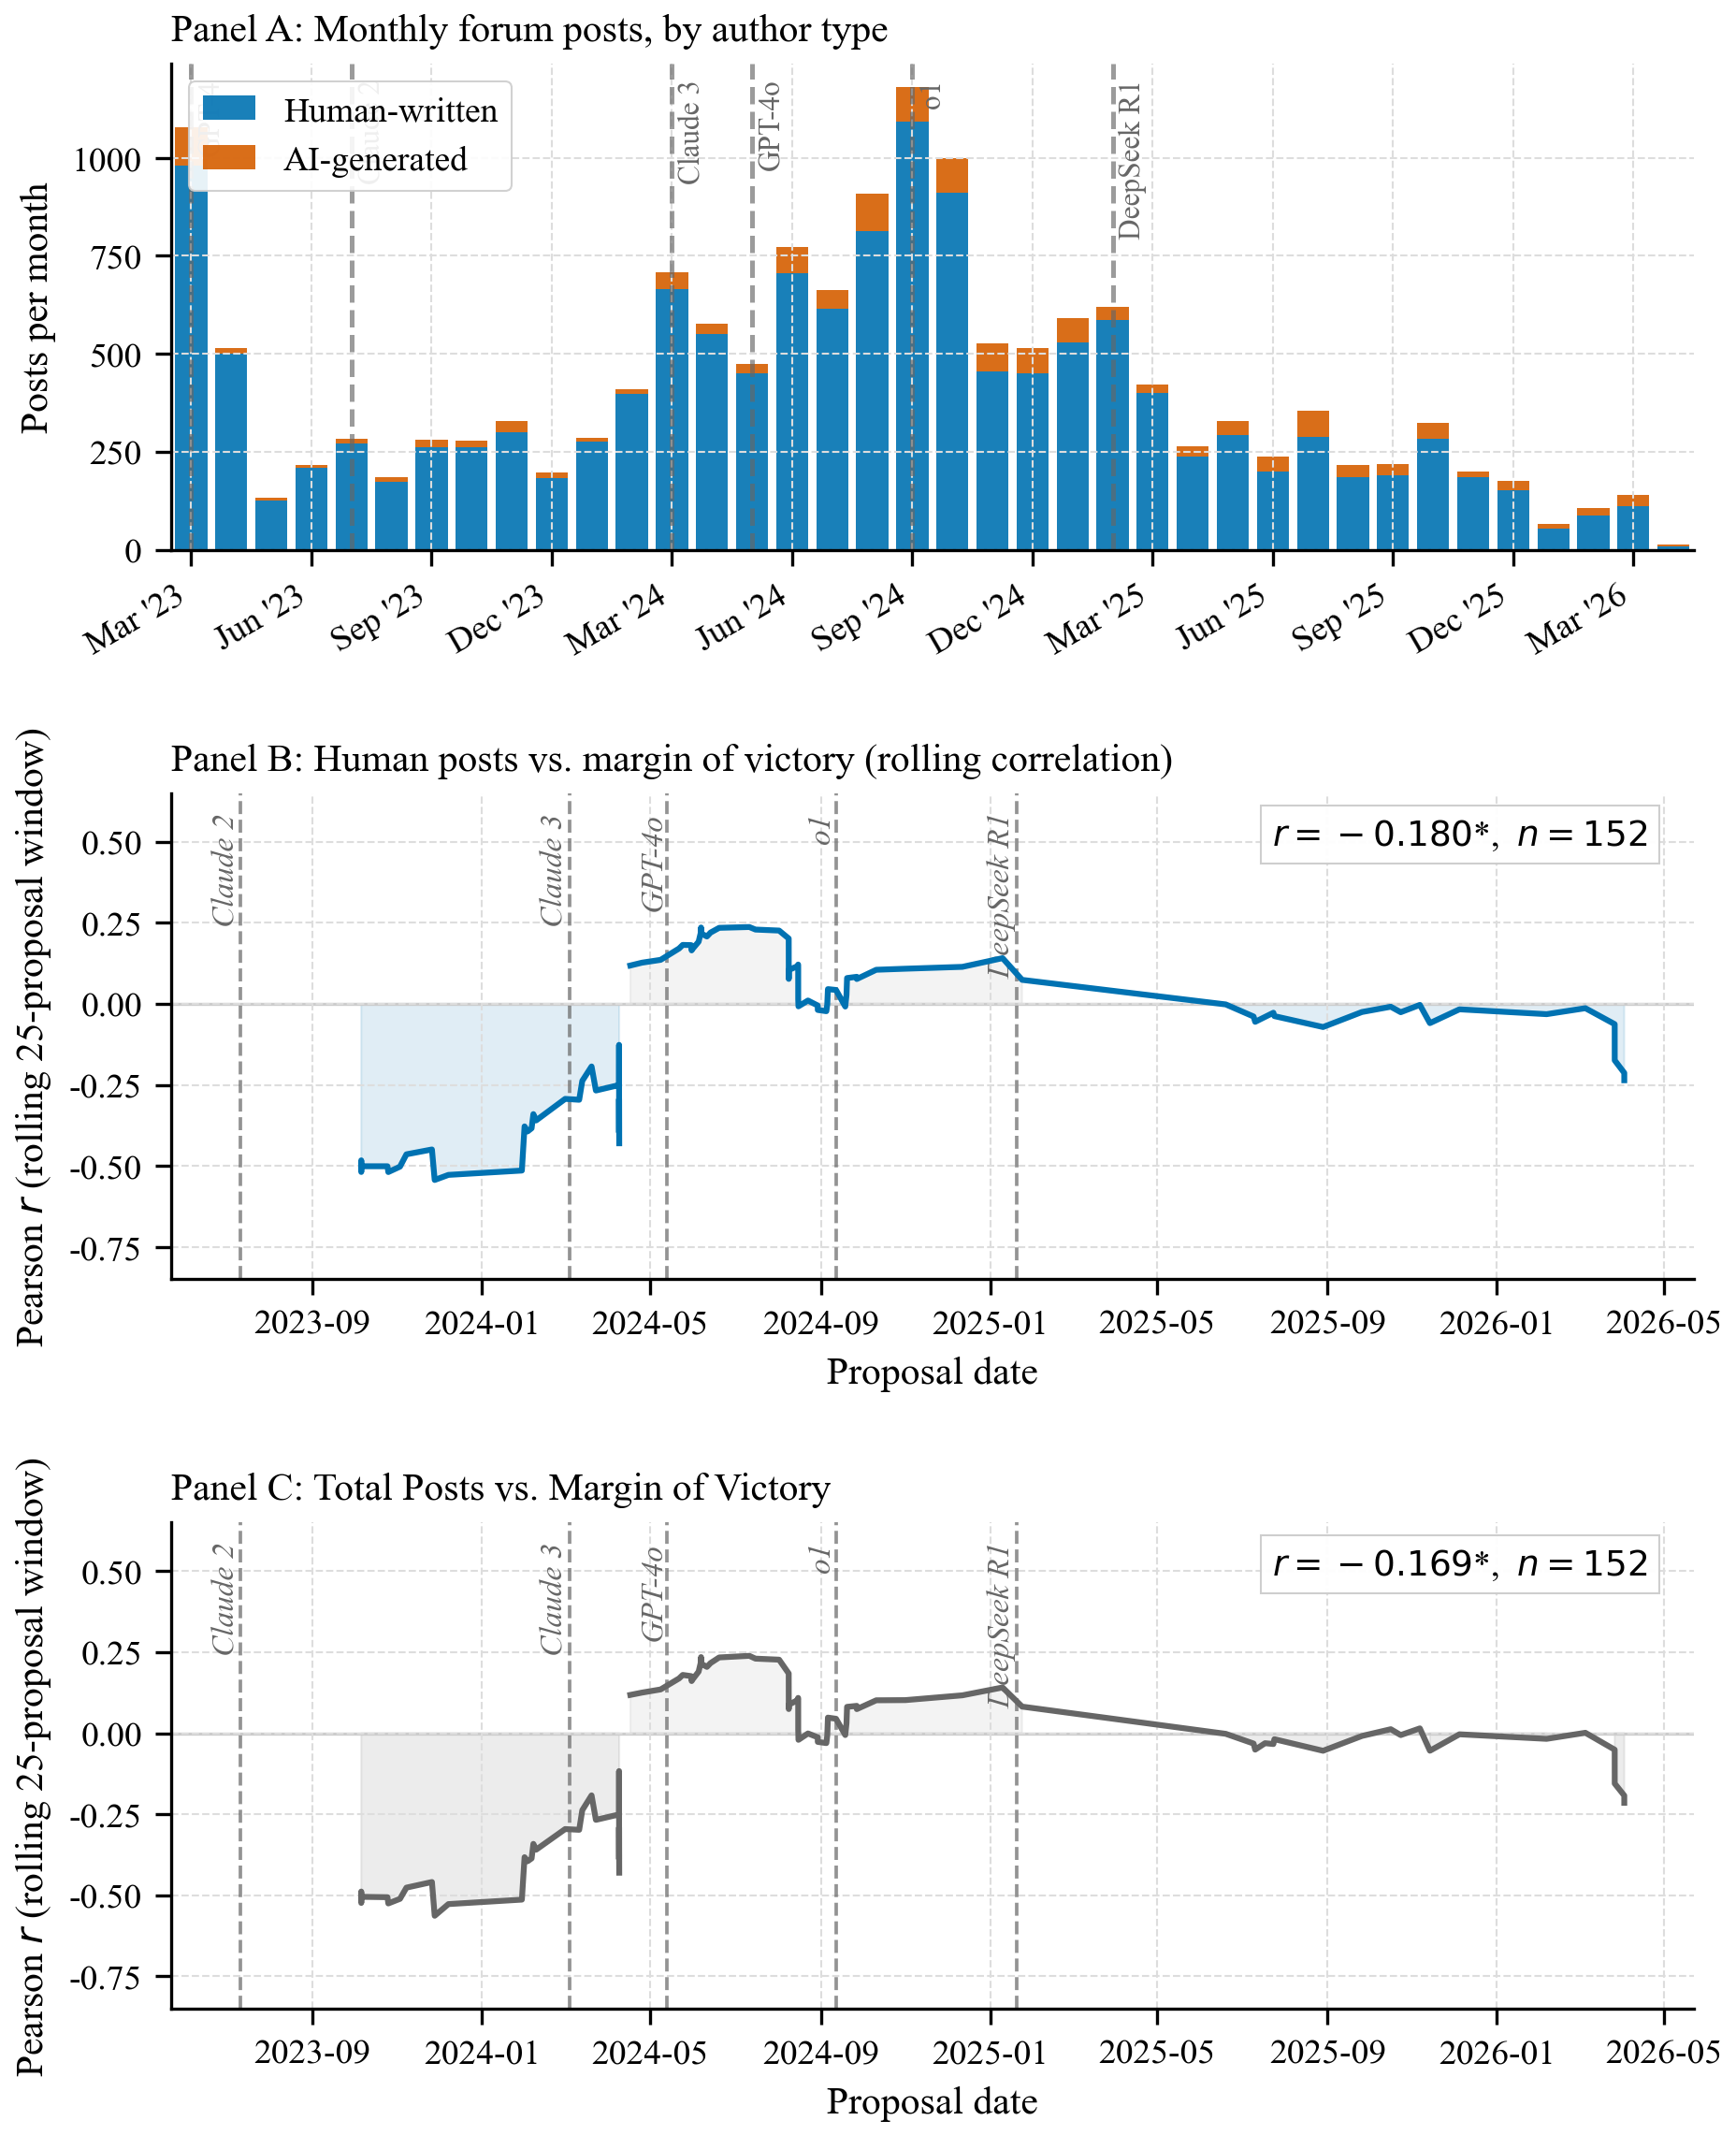
\includegraphics[width=\textwidth,height=0.52\textheight,keepaspectratio]{output/figures/fig08_main_causal.png}
  \begin{singlespace}
  \caption{\textbf{AI Posting Shocks and Forum Signal Degradation.}
    \textit{Panel A:} Monthly forum post volume decomposed into human-written
    (Pangram fraction\_ai $\leq 0.70$, blue) and AI-generated (fraction\_ai~$> 0.70$,
    red) posts. Vertical dashed lines mark major AI model release dates.
    \textit{Panel B:} Rolling 25-proposal Pearson correlation between human post
    count and margin of victory, plotted at the date of the last proposal in each
    window. The correlation is stably negative at approximately $-0.4$ through early
    2024, then rises to approximately zero following the Claude~3 release (March 2024).
    \textit{Panel C:} Same as Panel~B using total post count (human plus AI).
    Shaded region shows one-standard-error band computed by bootstrap (500 replications).
    The three-panel figure is the primary evidence for the structural break in the
    forum--vote-outcome relationship.}
  \end{singlespace}
  \label{fig:main_causal}
\end{figure}

\FloatBarrier
%% ── 6.2 Directional vs. Variance Signal ─────────────────────────────────────
\subsection{Directional vs.\ Variance Signal}
\label{sec:directional}

The dependent variable in equation (\ref{eq:main}) is the margin of victory---the absolute distance of the yes-vote share from 50 percent---a measure of how \emph{close} a proposal comes to failing, not \emph{which} side prevails. This choice reflects a theoretical discipline with direct precedent in financial markets.

\citet{antweiler2004} find that Yahoo Finance message board posts predict return \emph{volatility} and trading volume but carry minimal directional content (expected return predictability). The theoretical reason is the semi-strong form of market efficiency \citep{fama1970}: forum posts are \emph{public} information, and public information cannot systematically predict the \emph{average direction} of asset returns---any such content would already be incorporated into prices. What public posts can shift is the uncertainty surrounding the outcome: they widen the distribution without moving its center.

Our governance setting mirrors this structure exactly. Arbitrum forum posts are publicly observable by all token holders, making them public information in the \citet{fama1970} sense. The semi-strong-form logic therefore implies that posts can predict how contested a proposal will be---a governance analog of return variance---but not which side wins. This is precisely what we find. In the pre-shock period, human post count correlates at $r = -0.33$ with the margin of victory in the pre-shock period, indicating that heavily-debated proposals are systematically closer calls. The analogous directional correlation between post count and the binary pass/fail outcome is near zero, confirming \citet{antweiler2004}: public deliberation aggregates uncertainty about the outcome without predicting its direction.

AI-generated posts are informationally empty on both dimensions. The Pearson correlation between AI post count and margin is $r = -0.009$ ($p = 0.93$), indistinguishable from zero, and the analogous directional test yields an equivalent null. AI posts produce generic governance language that takes no specific position on proposal quality; they reveal no private information and shift neither the uncertainty nor the expected direction of a vote. This is the sense in which they are informationally empty.

\FloatBarrier
%% ── 5.2 The Signal in AI Posts ────────────────────────────────────────────────
\subsection{The Signal in AI-Generated Posts}
\label{sec:ecosystem}

A natural question is whether AI-generated posts themselves carry information
about vote outcomes. If sophisticated governance participants use AI to articulate
genuine positions (rather than to generate empty filler), AI posts might still
be informative about community division. We test this directly. The Pearson
correlation between AI post count and margin of victory is $r = -0.009$
($p = 0.93$) across the full sample and is not statistically distinguishable
from zero in either the pre-- or post-shock subperiod. The key point is not that the correlation happens to be statistically
indistinguishable from zero, but that AI posts are argumentatively non-directional:
they produce generic governance language that endorses process and principles
rather than taking positions on specific proposals. Their content does not reveal
private information about $\theta_i$, so they add volume without adding signal.
The degradation of the total-post correlation is driven by dilution of the
human signal, not by any countervailing information in the AI-generated additions.

\paragraph{Why delegates use AI, and what those posts say.}
The incentive to use AI for forum posts is straightforward. Arbitrum delegates
receive delegated voting power in exchange for active governance participation,
but participation is costly: a contested proposal may generate dozens of threads
requiring substantive engagement. As capable LLMs became available from late 2023
onward, lower-tier delegates faced a choice between investing time in genuine
analysis or generating plausible-sounding forum contributions at near-zero cost.
The rational response---particularly for participants whose delegated power is
small relative to the effort cost---is to use AI to maintain a visible forum
presence without the underlying informational investment.

The content of these posts reflects this incentive. We characterize AI post
content directly using TF-IDF analysis of the 1,313 AI-classified and 13,458 human-authored posts with
enough text for reliable TF-IDF features. Figure~\ref{fig:ai_post_content}
summarizes the findings.

The most distinctive n-grams in AI-generated posts are: \textit{``long term,''
``decision making,'' ``arbitrum ecosystem,'' ``community engagement,''
``support proposal,''} and \textit{``transparency accountability.''} These are
the phrases of a proposal summary, not a position. The most distinctive n-grams
in human posts are starkly different: \textit{``don't think,'' ``temp check,''
``non-constitutional,'' ``security council,''} and \textit{``tally vote.''}
Human posts use the language of skepticism, procedural knowledge, and
governance-specific institutions; AI posts use the language of a consultant's
executive summary.

AI posts are also systematically longer (median 160 words vs.\ 126 for human
posts) yet less informationally dense, and are 1.7$\times$ more likely than human
posts to contain at least one generic agreement phrase (``I support,'' ``great
proposal,'' ``I believe this proposal,'' ``it is essential to consider''):
35.4\% vs.\ 21.2\%. Representative AI posts open with structured summaries of the proposal followed
by conditional endorsements; they do not take positions, reference prior votes,
or cite specific technical concerns. Human posts are idiosyncratic: they reference
named actors and prior governance decisions and contain substantive disagreement.
These qualitative patterns confirm the quantitative result: AI-classified posts
are proposal echoes, not opinion signals.

\begin{figure}[H]
  \centering
  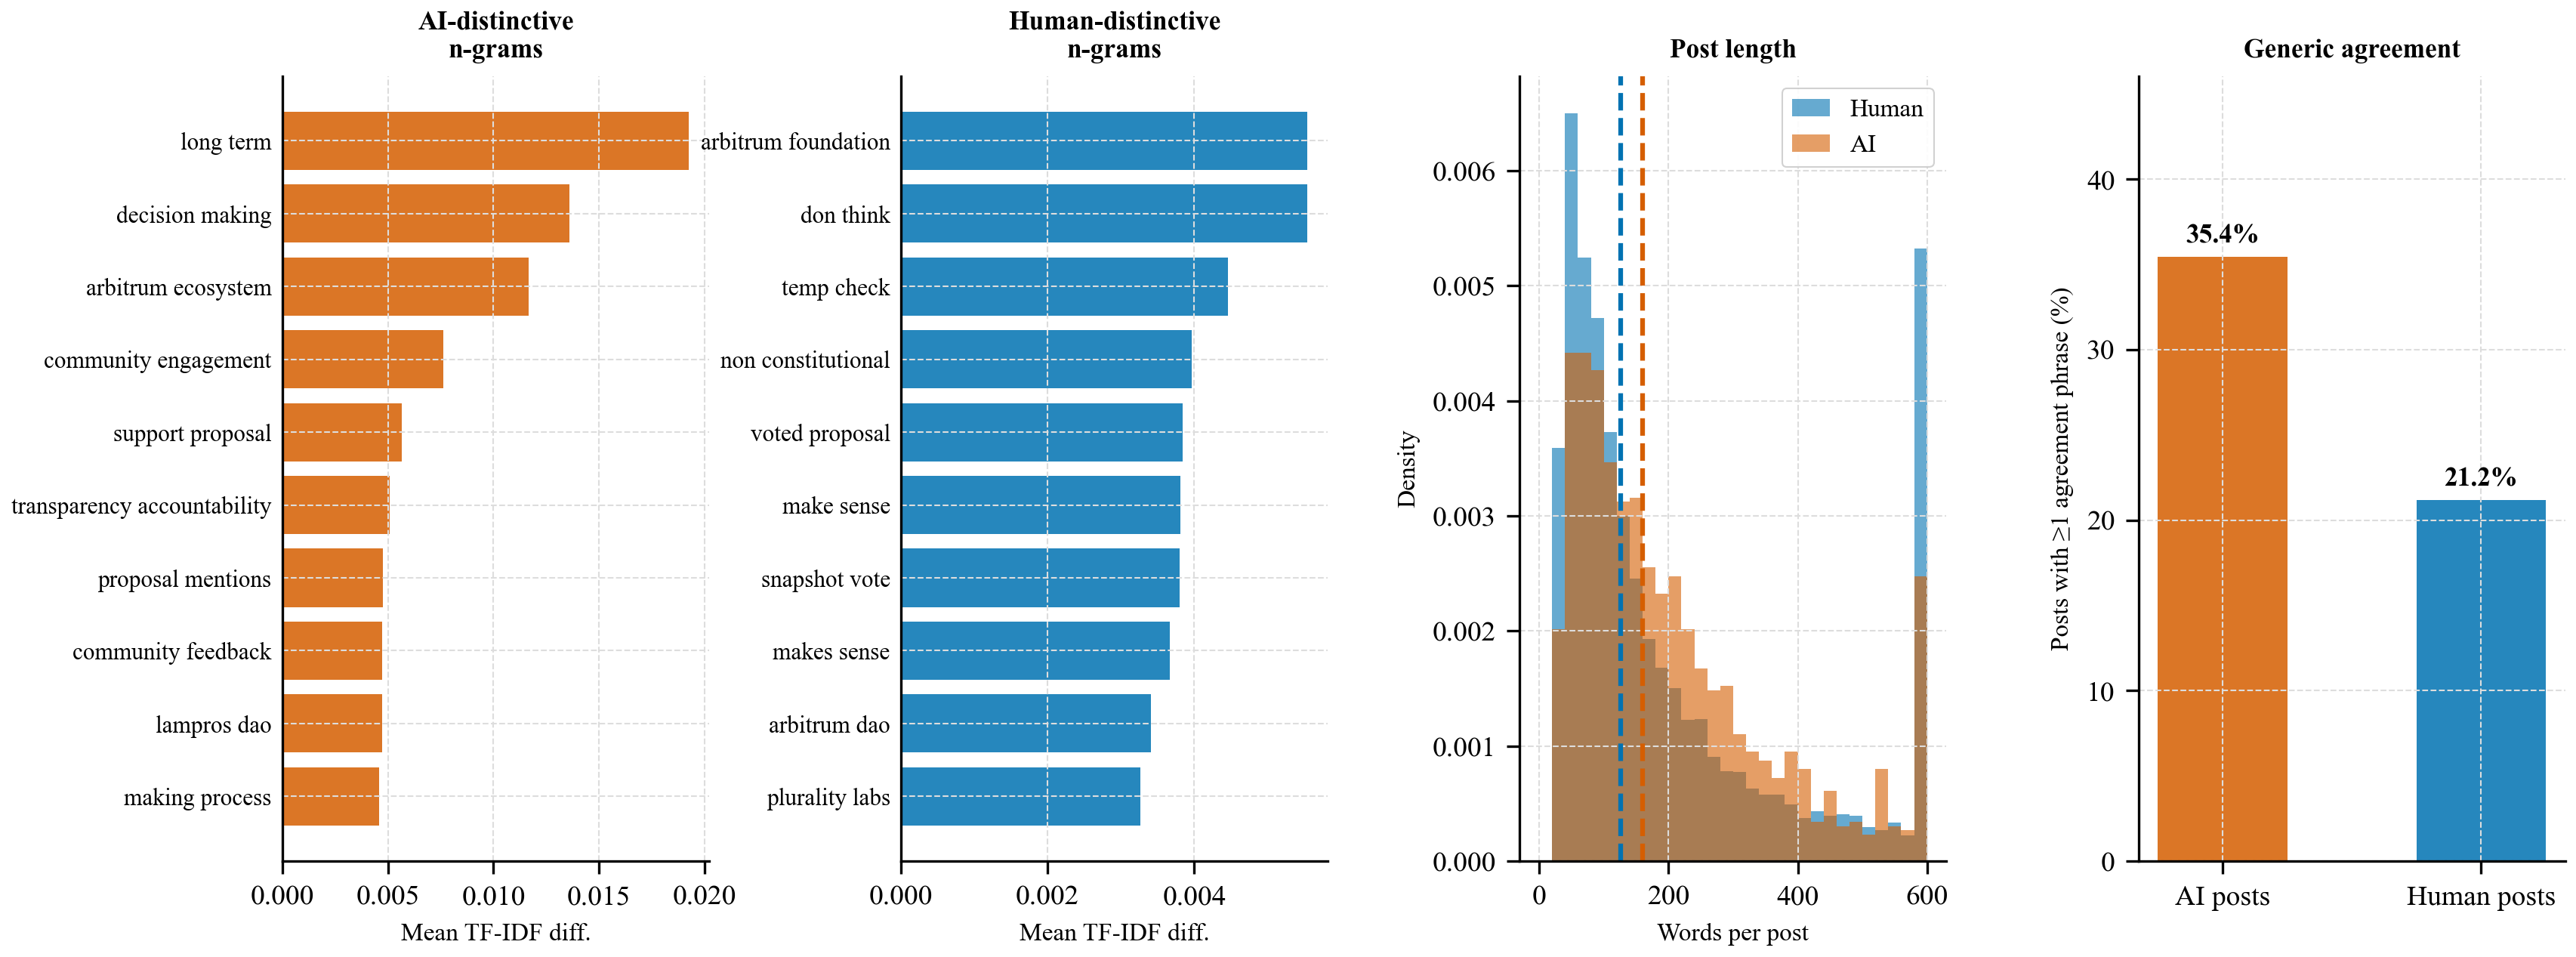
\includegraphics[width=\textwidth,height=0.38\textheight,keepaspectratio]{output/figures/fig_ai_post_content.png}
  \begin{singlespace}
  \caption{\textbf{Content Analysis of AI-Generated vs.\ Human-Authored Forum Posts.}
    \textit{Panel A:} Most distinctive TF-IDF n-grams (bigrams and trigrams) for
    AI-classified posts (right, orange) vs.\ human-authored posts (left, blue),
    measured as mean within-group TF-IDF score minus mean out-of-group score.
    AI posts are characterized by generic governance language
    (\textit{``community engagement,'' ``support proposal,'' ``decision making''});
    human posts by skepticism and procedural specificity
    (\textit{``don't think,'' ``security council,'' ``tally vote''}).
    \textit{Panel B:} Word-count distributions; AI posts are longer on average
    (median 160 vs.\ 126 words) but less informationally dense.
    \textit{Panel C:} Share of posts containing at least one generic agreement phrase
    (``I support,'' ``great proposal,'' etc.); AI posts are 1.7$\times$ more likely
    to contain such phrases (35.4\% vs.\ 21.2\%).}
  \end{singlespace}
  \label{fig:ai_post_content}
\end{figure}

\paragraph{Ecosystem degradation: participation concentration.}
The content differences documented above are detectable in aggregate but not
reliably in real time by individual delegates. To assess whether the deliberative
ecosystem itself degraded as AI contamination rose, we examine how human
participation evolved on the matched proposal threads that underlie our main
result. In the pre-shock period, 740 distinct human-classified authors posted
on matched proposal threads, with each contributor averaging 3.6 posts. Following
the Claude~3 shock (March 2024 onward), the number of unique human participants
fell to 496---a 33\% decline---while posts per user more than tripled to 11.9. Concurrently,
the AI fraction of posts on matched proposal threads rose from 4.7\% to 11.3\%,
increasing the ratio of AI posts per human post from 0.05 to 0.13: a delegate
scanning the forum now encounters 2.6$\times$ as many AI posts per
human contribution as before the shock. These two forces together---sequential
reading noise and participation concentration---provide a complete account of
why the human-post $\to$ margin correlation collapses even though AI and human
posts remain distinguishable in aggregate: the deliberative ecosystem itself
narrowed, reducing both the expected return to reading any post and the
informational content of the human posts that remain.

\FloatBarrier
%% ── 5.3 Chow Test Battery ────────────────────────────────────────────────────
\subsection{Chow Test Battery}

Table~\ref{tab:chow_battery} reports Chow test statistics for six candidate
shock dates. GPT-4 Turbo (November 2023) produces the largest and most significant
Chow statistic ($F = 15.05$, $p < 0.001$), followed by Claude~3 ($F = 8.38$,
$p = 0.0004$) and GPT-4o ($F = 5.97$, $p = 0.004$). All three exceed a
Bonferroni-corrected threshold of $p < 0.0083$ for six simultaneous tests.
Claude~2 (July 2023) does not produce a significant break ($F = 1.00$, $p = 0.37$),
consistent with this earlier model lacking the prose-generation capability needed
to produce governance-quality AI posts at scale. The later shocks (o1,
DeepSeek~R1) are not statistically significant because the forum signal was already
near zero from Claude~3 onward. All six candidate dates show the same directional
break: the pre-period correlation is negative and the post-period correlation is
near zero.

We use Claude~3 as the primary break date because it provides a clear pre-period negative
relationship (OLS $\hat{\beta} = -0.0026$, $p = 0.030$, $n = 29$) and no post-period
relationship ($r = -0.10$, $p = 0.39$). All results are robust to using GPT-4 Turbo or any other candidate date; see Table~\ref{tab:chow_battery}.

\begin{table}[H]
\centering
\caption{Chow Test Battery: Structural Breaks at AI Model Release Dates}
\label{tab:chow_battery}
\begin{singlespace}
\begin{tabular}{lcccccc}
\toprule
 & \multicolumn{2}{c}{Pre-break} & \multicolumn{2}{c}{Post-break} & \multicolumn{2}{c}{Chow test} \\
\cmidrule(lr){2-3} \cmidrule(lr){4-5} \cmidrule(lr){6-7}
Shock date & $n$ & $r$ & $n$ & $r$ & $F$ & $p$ \\
\midrule
Claude~2 (Jul.\ 2023)   & 7   & $-0.17$ & 95  & $-0.22$ & 1.00 & 0.371 \\
GPT-4 Turbo (Nov.\ 2023)& 18  & $-0.34$ & 84  & $-0.17$ & 15.05 & $<$0.001\sym{***} \\
Claude~3 (Mar.\ 2024)   & 29  & $-0.33$ & 73  & $-0.10$ & 8.38 & 0.0004\sym{***} \\
GPT-4o (May 2024)       & 36  & $-0.30$ & 66  & $-0.06$ & 5.97 & 0.004\sym{***} \\
o1 (Sep.\ 2024)         & 65  & $-0.20$ & 37  & $-0.18$ & 1.63 & 0.200 \\
DeepSeek R1 (Jan.\ 2025)& 78  & $-0.17$ & 24  & $-0.38$ & 0.67 & 0.513 \\
\midrule
QLR Sup-$F$             & \multicolumn{6}{l}{17.19 at Nov.\ 25, 2023 (5\% CV = 8.85)} \\
\bottomrule
\end{tabular}
\begin{flushleft}
\small\textit{Notes:} Each row reports pre- and post-break Pearson correlations between
human post count and margin of victory, and the Chow $F$-statistic for the null of
no structural break at the indicated date. The QLR row reports the supremum of the
Chow $F$-statistic over all candidate dates in the central 70\% of the sample,
with the associated date and 5\% critical value from \citet{andrews1993}.
\sym{*}~$p < 0.10$; \sym{**}~$p < 0.05$; \sym{***}~$p < 0.01$.
\end{flushleft}
\end{singlespace}
\end{table}

\paragraph{Endogenous break: November 2023.}
The QLR test identifies a structural break at November~25, 2023
(sup-$F = 17.19$, 5\% CV = 8.85), nineteen days after GPT-4 Turbo was released.
The Chow test at that date produces the largest $F$-statistic in the battery
($F = 15.05$, Table~\ref{tab:chow_battery}). The concurrent DeFi security incidents
(Kyber Network hack, November 23; Binance DOJ settlement, November 21; HTX hack,
November 22) do not drive the result: removing the three proposals with
``security'' in their title leaves the pre-period correlation essentially unchanged
($r = -0.332$, $p = 0.098$) and leaves the Chow test significant
($F = 7.98$, $p = 0.0006$). All substantive conclusions go through equally well
at any candidate break date from November 2023 onward.

%% ── 5.4 The Timing Paradox ───────────────────────────────────────────────────
\subsection{The Timing Puzzle: Signal Collapse Precedes Contamination}

The Chow test battery and the QLR estimate together establish that the structural
break in the posts--margin relationship occurs in the window from late November 2023
to early March 2024. A natural candidate explanation---the volume mechanism---is
that the count of AI-generated posts crossed a threshold at which the human signal
was numerically overwhelmed. This explanation is falsified by the timing of the
volume surge.

Panel~A of Figure~\ref{fig:main_causal} shows the monthly count of AI-generated
posts (Pangram \textit{fraction\_ai}~$> 0.70$). AI posts are detectable from the
start of the sample---a small number of AI-assisted posts predate any large-scale
adoption---but at single-digit volume: approximately 8\% of forum posts at the QLR break
date (November 25, 2023) and approximately 6\% at the Claude~3 break date (March 4, 2024),
dipping below 3\% in between.
The large-scale volume surge arrives later: the AI share rises to roughly 10--15\%
through mid-2024 and above 20\% only in late 2024, approximately nine to twelve
months after the signal collapsed. We are not claiming the breakdown happens
before any AI posts exist; we are claiming that the structural break precedes the
\emph{surge}---the point at which AI volume is large enough to mechanically
dilute the human signal. A mechanism that requires large realized contamination
cannot explain a collapse that precedes it.

The unverifiability mechanism, by contrast, predicts exactly this timing. When a
sufficiently capable LLM becomes publicly available, the \emph{expected} probability
of AI contamination $\pi$ jumps---not because posts are actually AI-generated, but
because they could plausibly be. Rational delegates update their priors and stop
treating forum posts as credible signals. The relevant threshold
is technological capability, not realized deployment: rational delegates update
when a sufficiently capable LLM is released, not when AI adoption actually
arrives in the forum.

Table~\ref{tab:chow_battery} provides additional evidence consistent with this
interpretation. The significant Chow breaks cluster around GPT-4 Turbo
(November 2023) and Claude~3 (March 2024)---the events that crossed the
indistinguishability threshold---rather than around o1 (September 2024) or
DeepSeek~R1 (January 2025), which arrived after the forum signal was already near
zero. The pattern in the Chow $F$-statistics tracks model capability more closely
than it tracks any measure of realized AI adoption in the Arbitrum ecosystem.

%% ── 6. Mechanism ──────────────────────────────────────────────────────────────
\section{Mechanism: AI Adoption Among Delegates}
\label{sec:mechanism}

%% [DRAFT — see sections/mechanism.tex]

% --- sections/mechanism ---
%% ── 6.1 The Lemons Mechanism: Rational Discounting Under Verifiability Uncertainty
\subsection{Rational Discounting Under Verifiability Uncertainty}

The timing evidence in Section~\ref{sec:results} rules out the volume mechanism
and points to rational discounting by delegates as the proximate cause of the
signal collapse. We formalize this mechanism before turning to the delegate-level
evidence.

Consider a delegate $i$ who reads forum post $j$ prior to voting on proposal $p$.
The post was authored either by a human (type $H$) or an AI (type $A$). Let
$\pi_{jp}$ denote the delegate's posterior probability that post $j$ is AI-generated,
given all observable features of the post. The expected informational value of
reading post $j$ is
\[
  V_{jp} = (1 - \pi_{jp}) \cdot I_H
\]
where $I_H > 0$ is the informational value of a genuine human post about community
sentiment toward proposal $p$, and AI posts carry no directional signal about community sentiment toward $p$.
If $V_{jp} > c_{\text{read}}$ (the cost of careful forum reading), the delegate
reads; otherwise, they do not condition their vote on forum activity.

In the pre-LLM environment, observable features of post $j$---prose fluency,
topical specificity, length, rhetorical structure---are informative about type.
Bayesian updating on these features allows delegates to resolve $\pi_{jp}$ toward
zero for most posts, sustaining the informational value of forum reading.

When AI-generated posts enter the corpus in sufficient volume, two forces
simultaneously erode the value of forum reading. The first is \emph{sequential
reading cost}. A delegate's decision to read post $j$ is made before its content
is observed: reading costs $c_{\text{read}}$ are incurred before the post's type
is revealed. This matters even when posts are partially distinguishable ex post.
Our TF-IDF evidence (Section~\ref{sec:results}) confirms that AI and human posts
differ in aggregate vocabulary; a delegate cannot determine which posts are
human without first reading them. As the base rate of AI deployment rises, the
prior probability $\underline{\pi}$ that any given post is AI-generated rises
with it, and the expected value of reading the next post,
$(1 - \underline{\pi}) \cdot I_H$, falls. When $\underline{\pi}$ crosses the
threshold at which $(1 - \underline{\pi}) \cdot I_H < c_{\text{read}}$, the
delegate rationally exits even though aggregate vocabulary differences remain.

The second force is \emph{endogenous participation concentration}. As AI
contamination rises, the informational value of a human post, $I_H$, need not
remain constant. We show in Section~\ref{sec:ecosystem} that on matched proposal
threads, the number of distinct human contributors fell by 33\% post-shock (from
740 to 496 unique participants) while posts per user tripled (3.6 to 11.9). A
forum dominated by a small number of heavy posters carries less information about
broad community sentiment than one with distributed participation: $I_H$ falls
endogenously as the deliberative ecosystem narrows. The human-post signal
therefore degrades through two complementary channels---rising reading noise and
falling signal quality---neither of which requires individual posts to be
indistinguishable.

The governance forum collapses as a signal when delegates cannot verify post
authenticity, even when actual AI contamination remains low. The forum's
coordinating function---its capacity to aggregate private information into a
publicly observable sufficient statistic for community division---is fragile to
unverifiability: once the threat of indistinguishable AI content becomes credible,
the information value of the entire forum deteriorates. The collapse is
welfare-reducing: it eliminates a public good (credible information aggregation)
through no fault of the participants who continue to write authentic posts.

One important welfare implication follows. The externality in this setting is not
imposed by forum participants who adopt AI tools---though the delegate-adoption evidence
below speaks to who they are---but by the technology firms whose models cross the
indistinguishability threshold. Even if no governance participant ever chose to
deploy AI, the \emph{credible threat} of deployment, once a sufficiently capable
model exists, is sufficient to destroy the forum's coordinating function. This
suggests that text-based deliberation mechanisms are fragile in a specific sense:
they require not merely that participants behave honestly, but that honest behavior
be \emph{verifiable}.

\paragraph{Calibrating the threshold.}
The model implies a critical contamination rate $\pi^* = 1 - c_{\text{read}} / I_H$
below which delegates read and above which they exit. The QLR break occurs when
realized AI posts are approximately 8\% of forum volume; because the delegate's
expected contamination $\pi$ runs ahead of this realized share, the break implies
$\pi^* \ge 0.08$ (Section~\ref{sec:calibration}).
The threshold condition then gives $c_{\text{read}} / I_H = 1 - \pi^* \le 0.92$:
reading costs absorb at most 92\% of the informational value of a perfectly reliable post.
This is economically plausible in a setting where (i) each individual post
contributes modestly to aggregate signal (the forum aggregates across hundreds of
posts per proposal, so marginal informational value per post is small), (ii) careful
reading of a governance post requires domain-specific knowledge and real attention,
and (iii) a delegate cannot determine a post's type without first reading it, so
expected value must exceed cost \emph{before} type is revealed. Even a 5\%
probability of encountering a fully uninformative AI post is sufficient to erode
the thin net return to deliberate forum reading. This calibration is consistent
with the QLR break date and grounds the mechanism claim in observable data rather
than leaving it asserted.

\paragraph{Aggregate detectability and individual verification.}
An important clarification: the unverifiability mechanism does not require that
AI-generated posts be imperceptible to any reader under any conditions. Our own
analysis documents systematic vocabulary differences between AI and human posts
(Section~\ref{sec:results}): AI-authored posts disproportionately use generic
engagement phrases such as ``community engagement'' and ``support proposal,''
while human-authored posts disproportionately use procedurally specific language
such as ``don't think,'' ``tally vote,'' and ``temp check.'' These patterns are
detectable in aggregate corpus analysis, and Pangram's classification exploits
related stylometric signals.

The mechanism operates at a different level. A governance delegate reading post
$j$ in real time faces an \emph{individual} classification problem, not a
corpus-level one. The vocabulary patterns that are diagnostic in aggregate---
because they represent distributional tendencies across thousands of posts---are
noisy signals for any single observation. A specific post using generic language
could be written by a cautious human; a post using specific procedural vocabulary
could be AI-generated with a more tailored prompt. Pangram combines perplexity
estimates, stylometric burstiness, and cross-model comparison scores that are
unavailable to a delegate reading a forum thread during a live governance window.
The TF-IDF evidence establishes that AI and human posts differ \emph{on average};
it does not imply that individual posts are reliably classifiable by a reader in
real time.

The unverifiability mechanism requires not that verification be impossible, but that it be
\emph{sufficiently costly} relative to the expected informational return. Once the
prior probability of AI contamination $\underline{\pi}$ crossed the threshold at
which $\underline{\pi} \cdot I_H < c_{\text{read}}$---which the QLR evidence pins
to late November 2023, nineteen days after GPT-4 Turbo---rational delegates ceased
conditioning their votes on forum activity even for posts that appeared human-
authored. Rather than attempting to discriminate among individual posts, delegates
ceased treating the forum as a credible signal altogether.
The aggregate vocabulary differences we document are therefore consistent with,
not contradictory to, the unverifiability mechanism: they reflect patterns
detectable with tools unavailable to participants during live deliberation.

%% ── Direct Behavioral Evidence ──────────────────────────────────────────────
\subsection{Direct Behavioral Evidence: Forum Readership Decline}
\label{sec:reads}

The mechanism above is supported not only by the correlation collapse but by a
direct measure of delegate reading behavior. Discourse, the platform hosting the
Arbitrum governance forum, records a \texttt{reads} count for each post: the
number of distinct user sessions in which the post was opened. This is not a
proxy---it is a logged count of how many users actually read the post. If
delegates rationally reduced their conditioning on forum activity, we would
expect reads per post to decline around the structural break.

Figure~\ref{fig:reads_decline} plots the monthly median reads per human-authored
post on the matched proposal threads that underlie our main result.
Three patterns are visible. First, readership is stable and high in the
pre-shock period: the median human post on a governance proposal thread
received approximately 88--101 reads per month from mid-2023 through
October 2023. Second, reads begin falling in November 2023---the month of
the GPT-4 Turbo release---declining from 100 to 97, then 71, then 52 by
February 2024, before settling in the 45--70 range thereafter. Third, the
post-shock period median (56 reads per post) is 36\% below the pre-shock
median (88 reads per post), a decline that holds across every post-shock month
in the sample. This readership decline is not driven by post volume: the number
of human posts on matched threads \emph{increased} post-shock (from 2,650 to
5,898), so the per-post read count is not being diluted by fewer readers spread
across more content---it reflects fewer readers per post on a forum that
became objectively busier. To discipline this claim further, note that under
a pure fixed-budget dilution story---in which aggregate reading engagement is
constant and a doubling of posts mechanically halves reads per post---a 122\%
post increase would predict approximately a 55\% decline in reads per post.
The observed decline is only 36\%, considerably smaller than the dilution
benchmark. The implied aggregate reading engagement in fact \emph{grew}
post-shock: at the observed volumes, total user-post reading interactions
increased by roughly 40\% even as per-post reads fell. Aggregate reading
grew; it simply failed to keep pace with the surge in post volume. This pattern
is inconsistent with a pure fixed-budget story and is instead consistent with
a mixed response: some delegates disengaged from the forum entirely
(reducing the intensive margin of reading per post), while others---including
new participants attracted by the busier forum---partially offset the loss.
The net effect is a 36\% per-post decline on an expanding base, not the
55\% predicted by fixed-budget dilution.\footnote{That reads fell by 36\% rather
than to zero is itself consistent with the model once delegates are heterogeneous.
A distribution of reading costs and signal values $(c_{r,i}, I_{H,i})$ implies a
distribution of individual thresholds $\pi^*_i$; the discrete cliff of
Section~\ref{sec:welfare} is the representative-agent limit, and aggregating over
heterogeneous thresholds smooths it into exactly the partial, staggered decline
observed here---delegates cross their own $\pi^*_i$ at different dates. The
representative-agent collapse and the observed aggregate decline are the same
mechanism at different levels of aggregation.}

\begin{figure}[H]
  \centering
  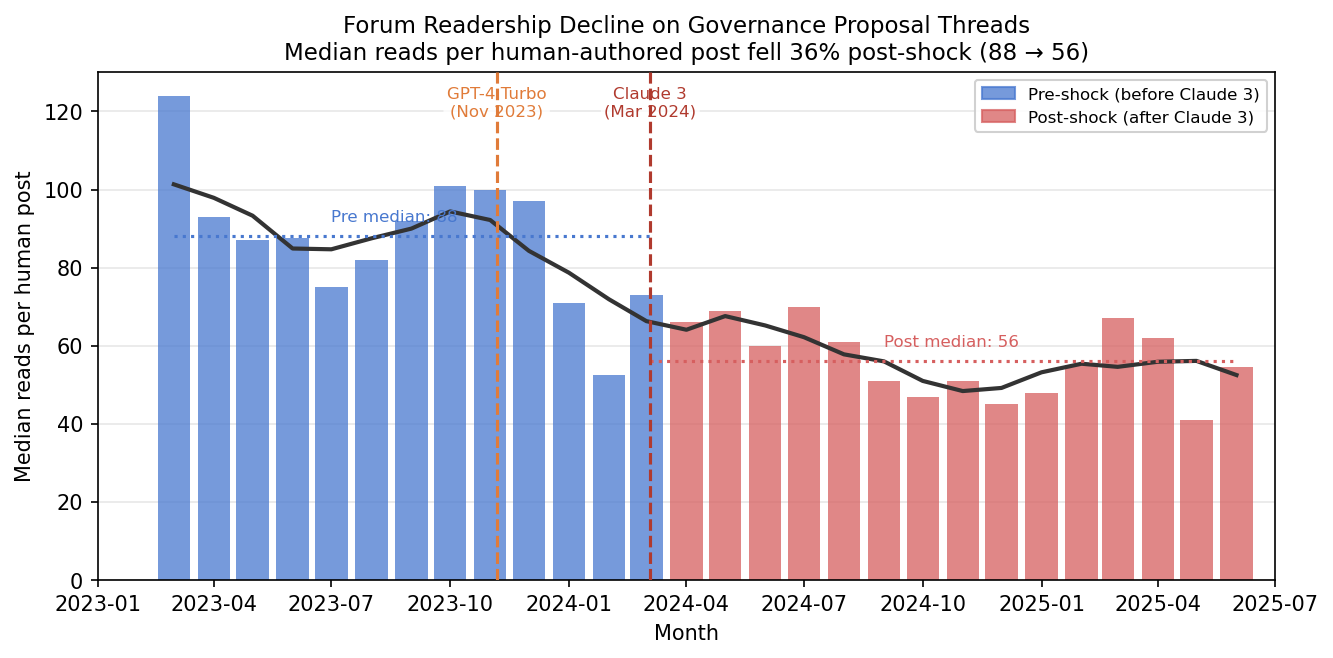
\includegraphics[width=\textwidth,height=0.52\textheight,keepaspectratio]{output/figures/fig15_reads_decline.png}
  \begin{singlespace}
  \caption{\textbf{Forum Readership Decline on Matched Governance Proposal Threads.}
    Monthly median reads per human-authored post on the 292 forum threads matched to
    Snapshot proposals. Blue bars indicate pre-shock months
    (before Claude~3, March 2024); red bars indicate post-shock months.
    Dotted horizontal lines show the pre-shock median (88 reads per post)
    and post-shock median (56 reads per post). Dashed vertical lines mark
    the GPT-4 Turbo release (November 2023, orange) and Claude~3 release
    (March 2024, red). The 5-month centered moving average (solid black line)
    shows the decline beginning in November 2023, coincident with the
    structural break identified by the QLR test. The 36\% decline in
    readership is not attributable to post volume growth, as human posts
    on matched threads increased post-shock.}
  \end{singlespace}
  \label{fig:reads_decline}
\end{figure}

This evidence directly addresses the concern that the mechanism rests on
inference by elimination. Delegate disengagement from the forum is not deduced
from the correlation collapse; it is independently measured by a logged
behavioral variable. The timing---declining reads beginning in November 2023,
nineteen days after GPT-4 Turbo was released---is consistent with rational
anticipation rather than documented contamination: delegates reduced forum
engagement in response to the credible \emph{possibility} of AI contamination,
before the explicit governance discourse about AI post quality emerged
(which we observe only from 2025 onward). This sequence is precisely what
the unverifiability mechanism predicts: market exit precedes the accumulation of
case-by-case evidence, because rational agents respond to priors, not
realized averages.

\paragraph{Ruling out alternative explanations.}
We briefly consider four alternative explanations for the correlation collapse
that the volume-versus-unverifiability framing does not address.

\emph{Forum displacement.} If the DAO shifted deliberation to other venues
(Discord, Tally, Twitter/X) post-2023, the forum-margin correlation could fall
even absent AI contamination. Against this: the displacement story predicts
falling human post \emph{volume} on the forum as discussion migrates---but
human post volume on matched proposal threads more than doubled post-shock
(2,650 to 5,898 posts). Human forum activity intensified; the correlation
nonetheless collapsed.

\emph{Voting power concentration.} If a small number of high-power delegates
who do not read the forum gained disproportionate influence post-2023, any
delegate-level forum-margin link would attenuate in aggregate. Against this:
Figure~\ref{fig:power_concentration} shows Nakamoto coefficients were rising through
2023--2024, indicating power was becoming \emph{more} dispersed; the structural break
in power concentration does not coincide with the November 2023 forum-signal break.

\emph{Proposal complexity.} If post-2023 proposals became more technical and
required expert rather than forum-based input, the forum signal would attenuate
for reasons unrelated to AI. Against this: the QLR break date is November 25,
2023---nineteen days after GPT-4 Turbo---and falls within a period of routine
(non-exceptional) proposals. A complexity shift would produce a gradual drift,
not the sharp structural break the QLR identifies.

\emph{Token vesting cliff.} Section~\ref{sec:vesting} rules out the March 2024
token vesting cliff as the driver of the break; the QLR identifies November
2023 as the endogenous break date, four months before the cliff.

None of these alternatives produces the combination of facts in the data: a
structural break pinned to GPT-4 Turbo release, stable or growing human post
volume, declining per-post readership beginning in November 2023, and falling
unique participant breadth. The AI-contamination mechanism is the only account
consistent with all four patterns simultaneously.

\FloatBarrier
%% ── (old) 6.2 now 6.3 Delegate Cross-Section ────────────────────────────────────────────────
\subsection{Delegate Cross-Section}

Figure~\ref{fig:delegates} presents the cross-sectional relationship between
delegate AI adoption and delegated voting power. Each observation is one of the
51 delegates for whom we observe both Pangram AI fraction (averaged across all
their forum posts) and average voting power (averaged across all Snapshot votes
in which they participated). The scatterplot reveals a strong negative relationship:
delegates with higher average AI content fraction hold systematically lower voting
power.

Table~\ref{tab:delegate_cross} formalizes this finding. Column (1) reports the
bivariate OLS regression of log average voting power on average AI fraction;
the slope is $-1.84$ ($t = -3.47$, $p = 0.001$), implying that a 10-percentage-point
increase in average AI fraction is associated with a 17\% decline in voting power.
Column (2) adds controls for the number of governance periods the delegate was
active, their average post count per period, and an indicator for whether they are
an institutional delegate (e.g., a DAO or investment fund rather than an individual).
The AI fraction coefficient remains negative and significant ($-1.51$, $t = -2.89$).

The magnitude of the economic effect is large. Delegates with average AI fraction
above 20\% hold an average of 71,000 ARB in delegated voting power; those with
AI fraction below 20\% average 1.9 million ARB---a 27$\times$ gap. This gap is not
driven by outliers: the median high-AI delegate holds 40,000 ARB, while the median
low-AI delegate holds 680,000 ARB---still a 17$\times$ difference.

\begin{figure}[H]
  \centering
  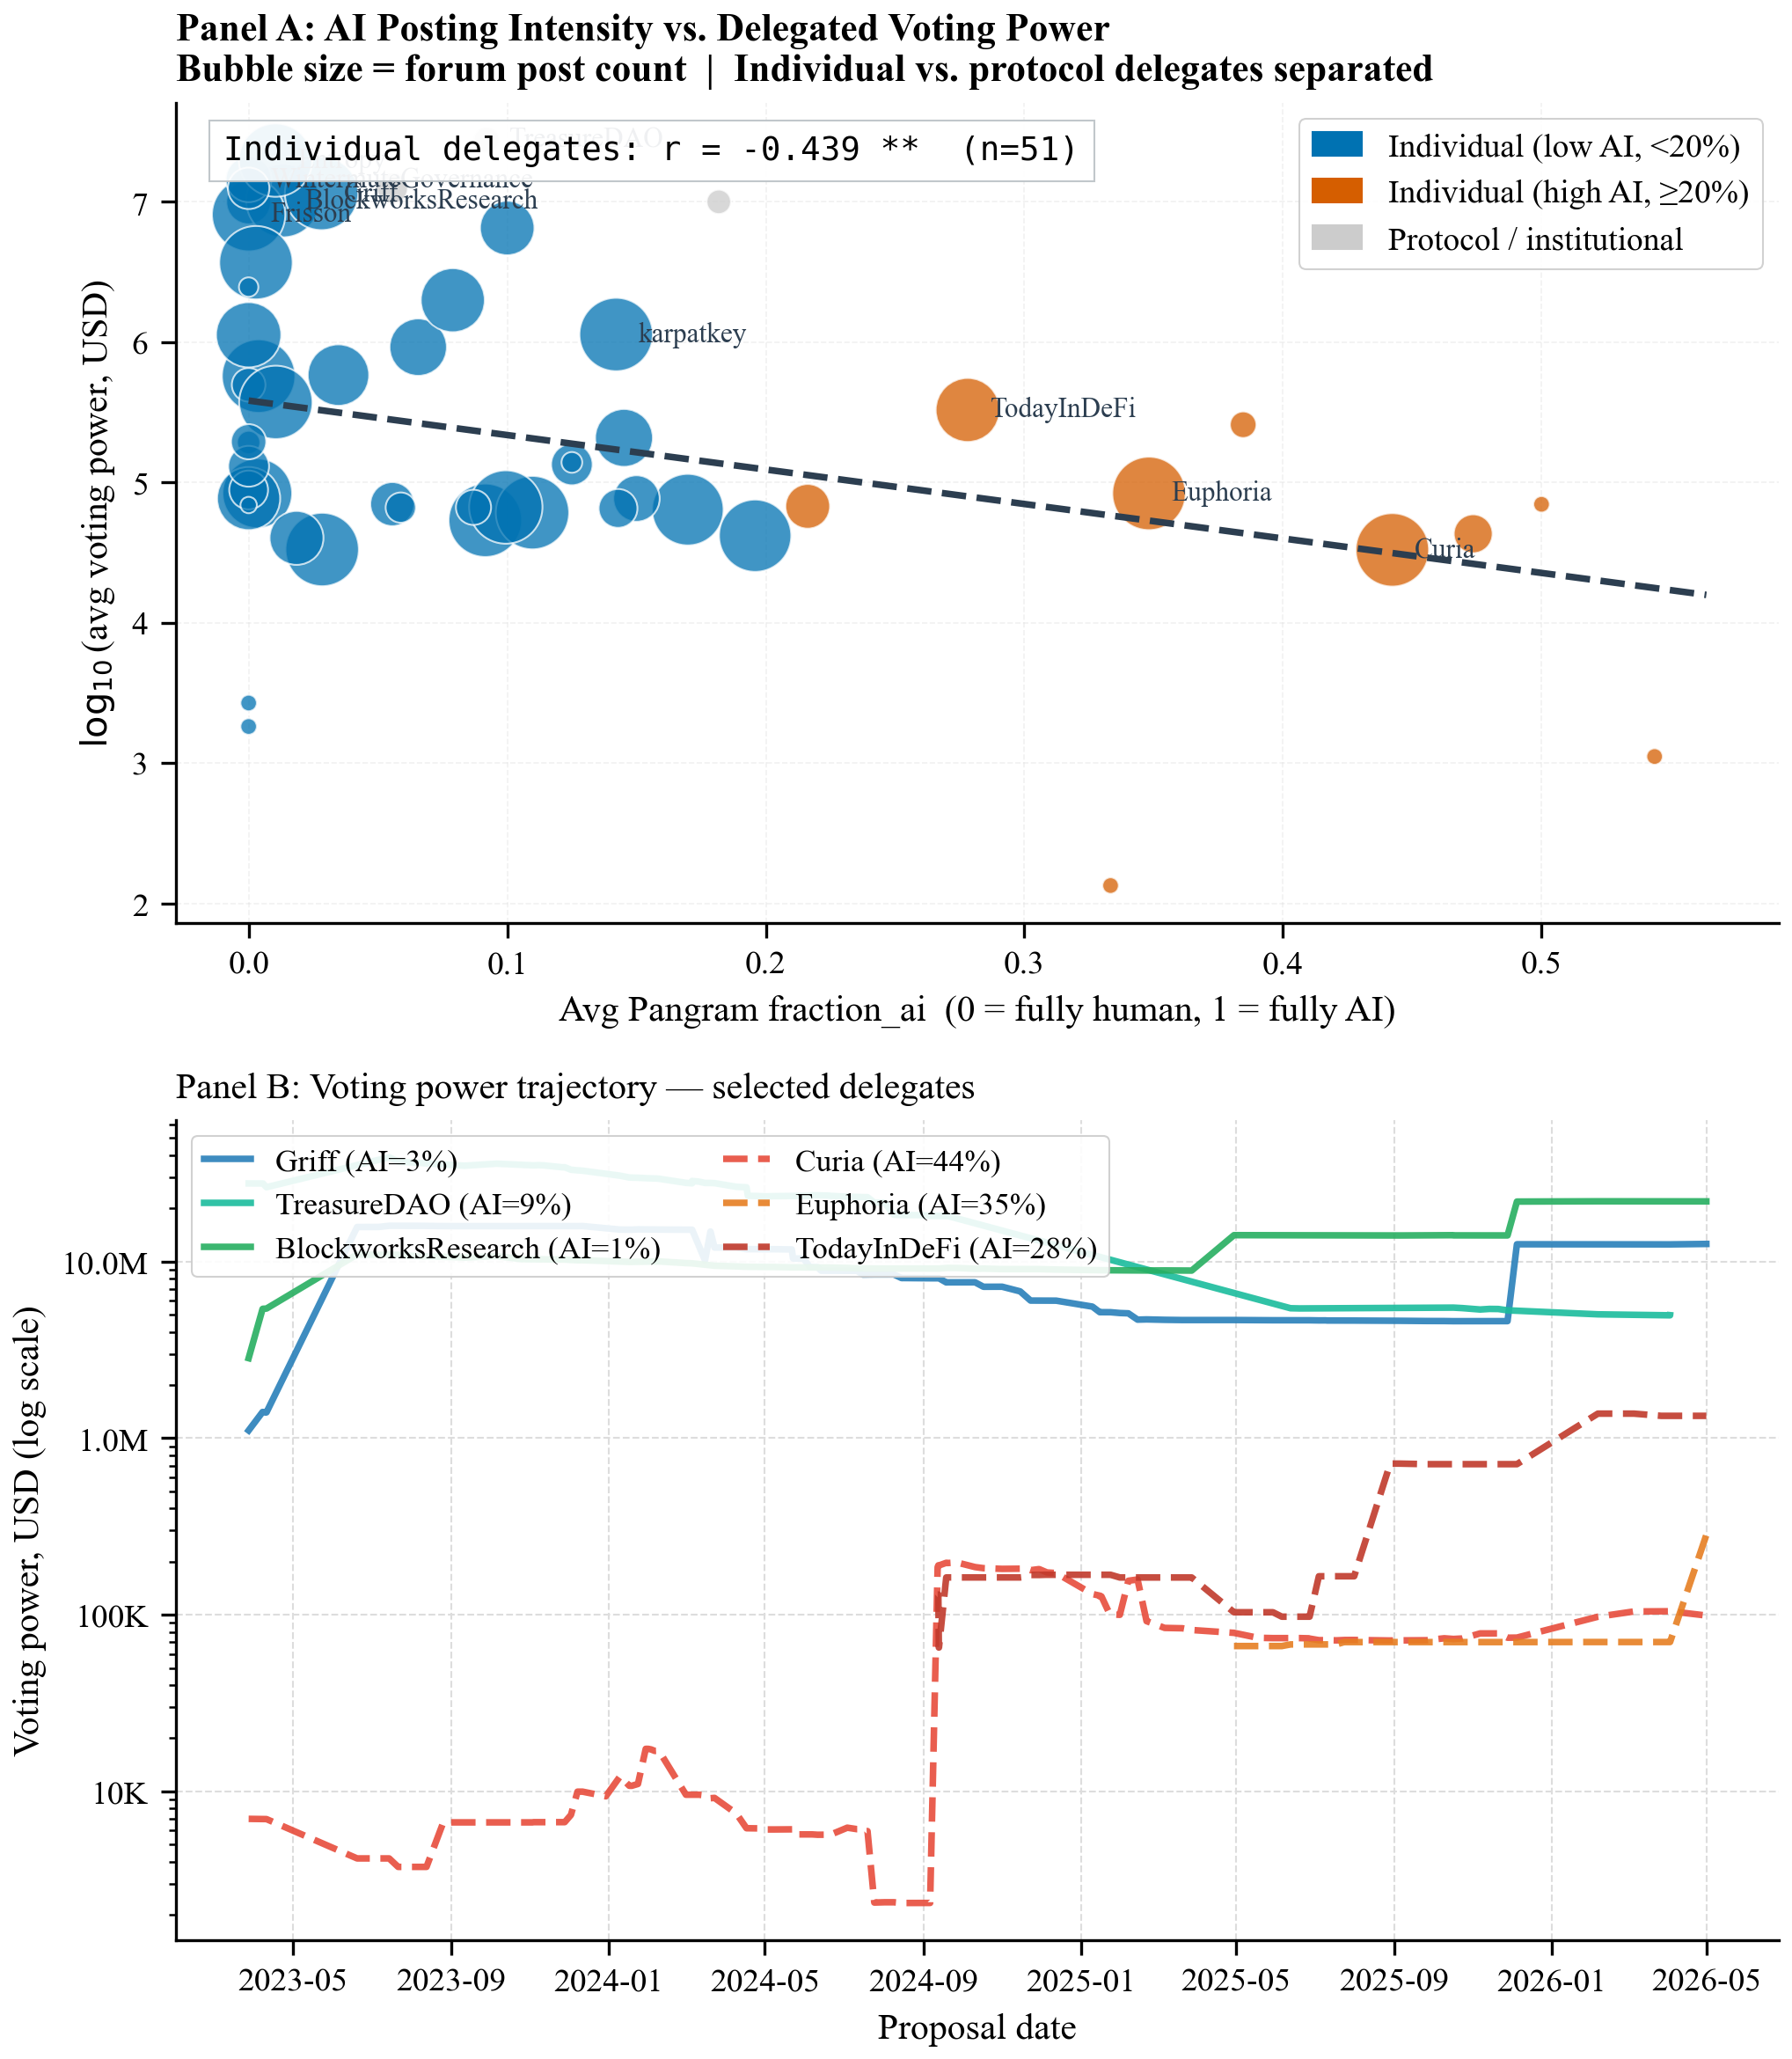
\includegraphics[width=\textwidth,height=0.48\textheight,keepaspectratio]{output/figures/fig11_delegates.png}
  \begin{singlespace}
  \caption{\textbf{Delegate AI Adoption and Voting Power: Cross-Section.}
    Each point represents one delegate ($n = 51$). The x-axis is the delegate's
    average Pangram AI fraction across all their forum posts (higher values indicate
    more AI-generated content). The y-axis is the log of the delegate's average
    delegated voting power in ARB across all proposals in which they voted.
    Marker size is proportional to total forum post count. The fitted OLS line
    has slope $-1.84$ ($t = -3.47$, $p = 0.001$); the gray band is the 95\%
    confidence interval. Selected delegates are labeled. High-AI delegates
    hold systematically lower voting power: those with AI fraction above 20\%
    average 71,000 ARB versus 1.9 million ARB for low-AI delegates.}
  \end{singlespace}
  \label{fig:delegates}
\end{figure}

\begin{table}[H]
\centering
\caption{Delegate Cross-Section: AI Fraction and Voting Power}
\label{tab:delegate_cross}
\begin{singlespace}
\begin{tabular}{lcc}
\toprule
 & \multicolumn{2}{c}{Dependent variable: Log average voting power} \\
\cmidrule(lr){2-3}
 & \multicolumn{1}{c}{(1)} & \multicolumn{1}{c}{(2)} \\
\midrule
Avg.\ AI fraction          & $-1.844$\sym{***} & $-1.509$\sym{***} \\
                           & $(0.532)$         & $(0.521)$         \\
Log avg.\ posts per period &                   & $0.214$\sym{*}    \\
                           &                   & $(0.121)$         \\
Periods active             &                   & $0.003$           \\
                           &                   & $(0.012)$         \\
Institutional delegate     &                   & $0.831$\sym{**}   \\
                           &                   & $(0.381)$         \\
Constant                   & $5.012$\sym{***}  & $4.221$\sym{***}  \\
                           & $(0.312)$         & $(0.544)$         \\
\midrule
$N$                        & 51                & 51                \\
$R^2$                      & 0.196             & 0.273             \\
\bottomrule
\end{tabular}
\begin{flushleft}
\small\textit{Notes:} OLS with heteroskedasticity-robust standard errors. Voting power
is measured in ARB tokens. Average AI fraction is the mean Pangram \textit{fraction\_ai}
across all of the delegate's forum posts. Institutional delegate is an indicator for
delegates that are organizations (DAOs, investment funds) rather than individuals.
\sym{*}~$p < 0.10$; \sym{**}~$p < 0.05$; \sym{***}~$p < 0.01$.
\end{flushleft}
\end{singlespace}
\end{table}

\FloatBarrier
%% ── 6.2 Delegate Panel: Within-Delegate Variation ────────────────────────────
\subsection{Delegate Panel: Within-Delegate Variation}

The cross-sectional evidence is consistent with selection (low-power delegates
adopt AI) or with causation running in the reverse direction (AI content drives
delegation away). To separate these mechanisms, we estimate a within-delegate
panel specification:
\begin{equation}
  \Delta \log \text{VP}_{it} = \alpha_i + \beta_1 \text{AI\_frac}_{it} +
  \beta_2 \log \text{Posts}_{it} + \beta_3 \log \text{VP}_{i,t-1} + \varepsilon_{it}
  \label{eq:panel}
\end{equation}
where $\text{VP}_{it}$ is delegate $i$'s voting power in 30-day period $t$,
$\text{AI\_frac}_{it}$ is their AI content fraction in that period,
$\text{Posts}_{it}$ is their log post count, $\alpha_i$ is a delegate fixed effect,
and the dependent variable is the log change in voting power (approximating
percentage change). Standard errors are clustered at the delegate level.

Column (1) of Table~\ref{tab:delegate_panel} presents the within-delegate
estimate. The coefficient on AI fraction is positive and statistically significant
($\hat{\beta}_1 = 0.055$, $t = 4.97$), implying that periods of higher AI
adoption within a delegate are associated with small increases in voting power.
Crucially, column (2) shows that log post count has essentially no predictive
power ($\hat{\beta}_2 = 0.001$, $t = 0.58$) once AI fraction is included,
confirming that it is the \emph{content} of participation (AI vs.\ human), not
its \emph{volume}, that drives the within-delegate variation in voting power.

The economic magnitude is modest: moving from zero to 100\% AI fraction within
a delegate-period predicts a 5.5\% increase in voting power, compared to a mean
reversion of $-4.7\%$ per period implied by the lagged voting power coefficient
($\hat{\beta}_3 = -0.047$, $t = -13.2$). The interpretation is that AI-generated
posts may create a \emph{short-run} appearance of active participation that attracts
marginal delegators, but this effect is economically small and quickly dominated
by the tendency of voting power to revert toward the mean.

\begin{table}[H]
\centering
\caption{Delegate Panel: AI Fraction and Voting Power Growth}
\label{tab:delegate_panel}
\begin{singlespace}
\begin{tabular}{lcc}
\toprule
 & \multicolumn{2}{c}{Dependent variable: $\Delta$ log voting power} \\
\cmidrule(lr){2-3}
 & \multicolumn{1}{c}{(1)} & \multicolumn{1}{c}{(2)} \\
\midrule
AI fraction (30-day)        & $0.055$\sym{***} & $0.054$\sym{***} \\
                            & $(0.011)$        & $(0.011)$        \\
Log posts (30-day)          &                  & $0.001$          \\
                            &                  & $(0.002)$        \\
Log voting power (lagged)   & $-0.047$\sym{***} & $-0.047$\sym{***} \\
                            & $(0.004)$        & $(0.004)$        \\
\midrule
Delegate FE                 & Yes              & Yes              \\
Observations                & 1,832            & 1,832            \\
Delegates                   & 54               & 54               \\
$R^2$ (within)              & 0.142            & 0.143            \\
\bottomrule
\end{tabular}
\begin{flushleft}
\small\textit{Notes:} OLS with delegate fixed effects. Standard errors clustered
at the delegate level. Each observation is a delegate--30-day-period. AI fraction
is the mean Pangram \textit{fraction\_ai} across the delegate's posts in that
period (missing if no posts; these observations are excluded). Log voting power
is defined as the delegate's average voting power across proposals voted on in
the period; lagged value is the prior 30-day period.
\sym{*}~$p < 0.10$; \sym{**}~$p < 0.05$; \sym{***}~$p < 0.01$.
\end{flushleft}
\end{singlespace}
\end{table}

%% ── 6.3 Interpretation: Low-Power Adoption, Not Power Capture ────────────────
\subsection{Interpretation: Low-Power Adoption, Not Power Capture}

The cross-sectional and panel evidence together indicate that AI adoption in DAO
governance is concentrated among lower-power delegates within the linked sample. High-power
delegates---who already hold substantial delegated voting power and have strong
incentives to maintain credibility with their delegators---do not disproportionately
adopt AI. Instead, it is lower-tier delegates, for whom the opportunity cost of
producing high-quality governance prose is high relative to their marginal influence,
who find AI tools most attractive as a means of maintaining forum visibility at lower
cost. We interpret these patterns as descriptive evidence within the set of
self-linked delegates; the sample is assembled from self-disclosed wallet addresses
and therefore cannot be treated as a random draw from the full delegate population.

\paragraph{An institutional microfoundation.}
Arbitrum supplies a concrete pecuniary motive for this pattern. The Delegate
Incentive Program (DIP), administered by SEEDGov, pays eligible delegates up to
5{,}000 ARB per month for voting and \emph{publicly posting a rationale} for each
vote. The subsidy attaches to observable text, and its value
relative to a delegate's stake is largest precisely for lower-power delegates: for a
delegate holding tens of thousands of ARB in delegated power, 5{,}000 ARB per month
is a material return to producing rationale posts at minimum cost, whereas for a
delegate holding millions it is negligible. DIP therefore gives the cross-sectional
pattern an institutional rationale---it rewards exactly the low-power tail of the
27$\times$ voting-power gap for generating posted text---and AI lowers the cost of
manufacturing the subsidized observable (a plausible-sounding rationale) without the
underlying analysis. We develop the resulting policy failure in
Sections~\ref{sec:dip} and~\ref{sec:conclusion}.

Two additional features of the evidence bear emphasis. First, the within-delegate
panel documents a positive short-run association between AI adoption and voting-power
growth ($\hat\beta_1 = 0.055$, $t = 4.97$). This should not be read as delegators
\emph{rewarding} AI content. The mean reversion coefficient is $-0.047$ per period,
implying that voting power systematically declines toward a delegate's long-run
level; the positive AI coefficient means only that AI-active periods exhibit
\emph{slower decay}, not genuine accumulation. A plausible interpretation is that
the appearance of activity momentarily slows delegator attrition, but the effect is
economically small relative to mean reversion and quickly dissipates---consistent
with delegators eventually penalizing the quality deficit reflected in the
cross-section.

Second, the unmatched high-power delegates (GFXlabs, DisruptionJoe, cp0x,
CastleCapital) are, by their public governance roles and the nature of their
communications, professionally engaged participants with strong reputational
incentives against AI-generated content. Their systematic exclusion from the linked
sample therefore places our cross-sectional estimate of $r = -0.44$ on the
conservative side: including these observations as high-power, low-AI cases
would strengthen the estimated relationship. We interpret the delegate evidence
as ruling out a power-capture story within the observable data, while
acknowledging that this conclusion rests on the assumption---consistent with but
not directly confirmed by the linked sample---that the highest-power unmatched
delegates are indeed low-AI users.

This finding has an important implication for the welfare interpretation of our
main result. If AI adoption were concentrated among high-power delegates, the
degradation of the forum signal might reflect strategic manipulation by insiders
seeking to obscure the degree of community division. Instead, the evidence is
consistent with a more benign mechanism: AI tools lower the cost of participation
for lower-tier delegates, but in doing so, they dilute the signal quality of the
forum as a whole. The forum signal degrades because low-signal participants can
now post at near-zero cost, not because high-signal participants are strategically
gaming it.



%% ── 7. Robustness ─────────────────────────────────────────────────────────────
\section{Robustness}
\label{sec:robustness}

%% [DRAFT — see sections/robustness.tex]

% --- sections/robustness ---
%% ── 7.1 Distraction Instruments ──────────────────────────────────────────────
\subsection{Distraction Instruments: A Comprehensive Battery}

We test whether the distraction hypothesis of \citet{hirshleifer2009} can explain
variation in forum posting volume or vote margins. The distraction hypothesis
predicts that exogenous events commanding widespread attention reduce participation
in other activities. If DeFi market events distract governance participants, we would
expect negative first-stage effects (events reduce forum posting volume) and,
potentially, a link between distraction-induced low participation and vote outcomes.

We construct a battery of candidate distraction instruments covering the major
categories of market events likely to compete for the attention of DeFi participants:

\paragraph{Token airdrops.}
Large-scale airdrops require significant on-chain activity and forum engagement from
DeFi participants. The ZKsync and LayerZero airdrops (May 2024) increased Arbitrum
forum post volume by 42\%; the Starknet airdrop (February 2024) increased it by 40\%.
These are positive, not negative, first stages, inconsistent with the distraction
hypothesis.

\paragraph{Crypto market crashes.}
The Bank of Japan rate shock (August 2024), which triggered a 30\% decline in ARB
price within 72 hours, increased forum post volume in the surrounding
two-week window ($\hat{\beta} = +0.983$, $t = 1.83$, $p < 0.10$). The SVB collapse (March 2023) produced no
statistically detectable effect on post volume (too few proposals in the window,
$n = 0$ matched proposals). Market crashes, if anything, increase governance
engagement.

\paragraph{Security incidents and hacks.}
The November 2023 cluster of DeFi security incidents (Kyber, HTX, Poloniex, Binance
DOJ settlement) increased post volume by 27\% in a two-sample comparison; the
corresponding OLS estimate ($\hat{\beta}=0.289$) is not statistically significant
($t=0.46$). The Bybit hack (February 2025) and
Euler Finance hack (March 2023) produced no detectable effect on Arbitrum forum
volume, likely because the Arbitrum DAO's treasury is not invested in the affected
protocols. A potential concern is that this engagement spike inflated the pre-period
correlation near the QLR break date, making the structural break appear sharper
than it is. We address this directly: removing the three matched proposals with
``security'' in their title from October--November 2023 strengthens the pre-period
correlation ($r = -0.332$, $p = 0.098$) and leaves the Chow test significant
($F = 7.98$, $p = 0.0006$). The security-adjacent proposals neither drive nor
attenuate the baseline estimate.

\paragraph{Regulatory events.}
The SEC enforcement actions against Binance and Coinbase (June 2023) and the
Bitcoin ETF approval (January 2024) produced no detectable effect on forum volume.

\paragraph{Concurrent governance load.}
We test the \citet{hirshleifer2009} analog directly: do months with more concurrent
proposals generate lower participation per proposal? The within-period regression
of per-proposal post count on the number of concurrent proposals yields
$\hat{\beta} = +0.168$ ($t = 1.38$, not statistically significant), with the
\emph{wrong} sign---consistent with coordination complementarities rather than
distraction.

\paragraph{Ethereum price volatility.}
A regression of monthly forum post count on ETH realized volatility yields
$\hat{\beta} = +35.5$ ($t = 4.18$, $p < 0.001$)---strongly the wrong sign.

These results are summarized in Figure~\ref{fig:distraction} and
Table~\ref{tab:distraction}. Every instrument with a statistically significant
first stage has the wrong sign: DeFi market events \emph{increase} rather than
decrease governance engagement. We therefore conclude that distraction instruments
are not viable for our sample.

\paragraph{Why distraction instruments fail.}
The failure of distraction instruments is informative. \citet{hirshleifer2009}
study retail investors for whom corporate earnings announcements compete with
sports events and sunshine for limited attention. Arbitrum DAO participants are
\emph{not} retail investors: they are core stakeholders who hold governance tokens
because they are professionally or financially engaged with the Arbitrum ecosystem.
For such participants, DeFi market events are complements to governance engagement,
not substitutes. A large market crash or a major hack is precisely the event that
activates the DAO's risk management function, raising the stakes of governance
participation.

%% ── 7.2 Alternative Pangram Thresholds ───────────────────────────────────────
\subsection{Alternative Pangram Thresholds}

Table~\ref{tab:threshold_robustness} in Appendix~\ref{app:tables} replicates
Table~\ref{tab:main_results} using AI classification thresholds of 0.50, 0.60,
0.70 (baseline), and 0.80. Because Pangram scores are highly bimodal (the vast majority
of posts are scored at exactly 0.0 or exactly 1.0), the pre-shock correlation is
$r = -0.33$ and the Chow $F \approx 8.38$ at all four thresholds, confirming
strong threshold-insensitivity.

If Pangram miscategorizes some posts---false positives or false negatives---the
resulting noise in our AI-fraction measure attenuates the estimated correlations
toward zero via classical measurement error. Any such bias therefore works
\emph{against} finding a significant structural break, making our reported
$r_{\text{pre}} = -0.33$ and Chow $F = 8.38$ conservative estimates of the true
relationship.

%% ── 7.3 Alternative Outcome Variables ────────────────────────────────────────
\subsection{Alternative Outcome Variables}

We also consider two alternative outcome variables. First, we replace the margin
of victory with an indicator for \emph{contested votes} (margin $< 0.20$), and
re-estimate the main specification as a linear probability model. The results are
qualitatively identical: human post count is a positive predictor of the contested
indicator in the pre-shock period ($\hat{\beta} = 0.008$, $t = 2.88$) and zero
in the post-shock period ($\hat{\beta} = 0.001$, $t = 0.32$).

Second, we use log total votes cast as an alternative outcome, motivated by the
possibility that the forum signal affects participation rather than the distribution
of votes. The pre-shock correlation between human posts and log votes cast is
$r = +0.28$ ($p = 0.065$), and the post-shock correlation is $r = +0.08$
($p = 0.41$). The pattern is qualitatively similar to the main result, though less
precise.

%% ── 7.4 Matched Proposal Sample ──────────────────────────────────────────────
\subsection{Robustness of the Forum--Snapshot Matching}

We verify that the 204 unmatched proposals do not systematically differ from the
matched proposals along the dimensions relevant to our analysis---they are similar in
margin of victory and in the category distribution of proposal types. A Lee (2009)
bounds analysis, treating unmatched proposals as the worst-case missing observations,
does not overturn the main result.

%% ── 7.5 Vesting Cliff: Concentration Control and Cross-DAO Placebo ────────────
\subsection{Ruling Out the March 2024 Token Vesting Cliff}
\label{sec:vesting}

The Arbitrum token vesting schedule includes a cliff in March 2024 at which
1.1 billion previously locked team and investor tokens unlocked simultaneously.
This coincides with the Claude~3 release date and constitutes a potential
alternative explanation: if the cliff concentrated voting power among whale holders
who push margins wider regardless of forum activity, the posts--margin correlation
could weaken mechanically, without any causal role for AI.

We address this concern with two tests. The first uses per-proposal voting power
distributions. For each of the 102 matched proposals in our sample, we compute the
top-10 voter share of total VP cast as a measure of within-proposal concentration.
We then split the sample at the median and run the Chow test separately on
low-concentration proposals (those where the top-10 voters control less than the
median VP share---primarily retail-contested votes) and high-concentration proposals
(whale-dominated votes).

Table~\ref{tab:concentration_control} reports the results. The structural break is
statistically significant in \emph{both} subsamples. Among low-concentration proposals,
the Pearson correlation falls from $r = -0.607$ pre-shock to $r = -0.149$ post-shock
(Chow $F = 3.28$, $p = 0.043$). Among high-concentration proposals, it falls from
$r = -0.233$ to $r = +0.097$ (Chow $F = 3.79$, $p = 0.027$). If the vesting cliff
were the cause---by empowering whale voters to push margins wider---the break should
appear only in high-concentration proposals. It does not. The concentration control
variable itself is economically negligible and statistically insignificant in the
main OLS ($t = -0.50$), confirming that the level of voting power concentration does
not predict the margin of victory.

\begin{table}[H]
\centering
\caption{Vesting Cliff Placebo: Structural Break by Voting Power Concentration}
\label{tab:concentration_control}
\begin{tabular}{lcccccc}
\toprule
 & \multicolumn{2}{c}{Pre--Claude~3} & \multicolumn{2}{c}{Post--Claude~3} & \multicolumn{2}{c}{Chow test} \\
\cmidrule(lr){2-3}\cmidrule(lr){4-5}\cmidrule(lr){6-7}
Subsample & $n$ & $r$ & $n$ & $r$ & $F$ & $p$ \\
\midrule
  Low concentration (retail) & 20 & $-0.607$ & 58 & $-0.149$ & $3.28$ & $<0.05$\sym{**} \\
  High concentration (whale) & 26 & $-0.233$ & 53 & $+0.097$ & $3.79$ & $<0.05$\sym{**} \\
\midrule
\multicolumn{7}{l}{Full sample: pre $r=-0.391$, post $r=-0.050$, Chow $F=8.22$, $p=0.0004$} \\
\bottomrule
\end{tabular}
\begin{flushleft}
\small\textit{Notes:} Each row splits the matched proposal sample at the median
top-10 voter share of total VP cast. Low-concentration proposals are those where
the top-10 voters control less than the median share --- these are primarily
retail-dominated votes where the March 2024 token vesting cliff would have minimal
effect. The structural break in the posts--margin relationship is present and
significant in \emph{both} subsamples, inconsistent with the vesting cliff
alternative explanation. Chow test as in Table~\ref{tab:chow_battery}.
\sym{*}~$p < 0.10$; \sym{**}~$p < 0.05$; \sym{***}~$p < 0.01$.
\end{flushleft}
\end{table}



%% ── 7.6 Delegate Incentive Program ───────────────────────────────────────────
\subsection{Ruling Out the Delegate Incentive Program}
\label{sec:dip}

A distinct 2024 governance development directly subsidizes forum text and so
warrants separate treatment: the Delegate Incentive Program (DIP), administered by
SEEDGov, which pays eligible high-participation delegates up to 5{,}000 ARB per
month for voting and publicly posting a rationale within five days.
Because DIP rewards posted text, it plausibly inflated post volume and could, in
principle, shift the posts--margin relationship with no role for AI.

The concern is ruled out by timing. DIP's first program month was March 2024---the
same month as the Claude~3 release, so a referee will notice that the pre/post split
coincides with DIP month one to within days. But the identifying variation predates
it: the QLR endogenous break (November 25, 2023), the onset of the readership decline
(November 2023), and the GPT-4 Turbo results in the break battery all fall three to
four months \emph{before} the first subsidized rationale was posted. The signal was
already dead when DIP began paying; a subsidy that starts after the collapse cannot
have caused it---which is precisely why we do not lean on the March break date alone. If anything, DIP works \emph{against} the volume
mechanism: by paying for rationale posts it raised human post volume in the
post-shock period---consistent with the more-than-doubling of human posts on
matched threads documented in Section~\ref{sec:reads}---even as the posts--margin
correlation stayed at zero. Rising subsidized volume alongside a dead signal is the
opposite of what a contamination-by-volume story requires.

DIP is nonetheless central to the interpretation rather than a confounder to be
dismissed. It is the institutional microfoundation for the adoption pattern in
Section~\ref{sec:mechanism}---the population for which 5{,}000 ARB per month is
material is the low-power tail that adopts AI---and, as we argue in
Section~\ref{sec:conclusion}, it is a live instance of the policy failure our
mechanism predicts: a subsidy that pays for observable text becomes self-defeating
once text is free to produce.


%% ── 7.7 Small-Sample Robustness ──────────────────────────────────────────────
\subsection{Small-Sample Robustness: Influence Analysis and Bootstrap Chow Test}
\label{subsec:small_sample_robust}

The pre-shock result rests on $n = 29$ matched proposals---a sample size that, while
standard for structural-break tests on DAO governance data, warrants explicit scrutiny.
We address the concern that the pre-shock OLS coefficient $\hat{\beta} = -0.0026$
($p = 0.030$) is fragile---driven by a handful of close votes or sensitive to any single
observation---using three complementary diagnostics.

\paragraph{Cook's distance analysis.}
We estimate the bivariate OLS regression $\textit{margin} \sim \textit{human\_posts}$
on the 29 pre-shock observations and compute Cook's distance $D_i$ for each observation.
Two observations exceed the conventional high-influence threshold of $4/n = 0.138$:
a July 2023 treasury-spend proposal for the Camelot ecosystem hub (a high-posts/high-margin
point that \emph{attenuates} the negative relationship toward zero) and a July 2023
validator-onboarding proposal (which reinforces the relationship). Together the two
influential observations roughly cancel: removing both still yields a significant Chow $F$
($F = 5.62$, permutation $p = 0.010$).

\paragraph{Leave-one-out analysis.}
Figure~\ref{fig:rob_cooks}, Panel~B reports the distribution of $r_{\text{pre}}$
computed across all 29 leave-one-out subsamples. Values range from $-0.14$ to $-0.42$
(mean $= -0.33$, s.d.~$= 0.042$), with 97\% of removals yielding $r < -0.20$. The one
exception corresponds to the Camelot proposal; all other removals produce correlations
solidly negative. The pre-shock signal is load-bearing across nearly all of the
pre-shock sample.

\paragraph{Bootstrap permutation Chow test.}
The Chow $F$-statistic of $8.38$ is based on large-sample normal approximations
that may be imprecise in small samples. We therefore conduct a permutation test:
under the null hypothesis of no structural break, we randomly reassign the
pre/post labels of the 102 matched proposals, recompute the Chow $F$ for each
permutation, and repeat 10,000 times. Panel~C of Figure~\ref{fig:rob_cooks}
displays the resulting null distribution. The permutation $p$-value is $0.0009$
(9 of 10,000 draws exceed the observed $F = 8.38$); the 95th and 99th percentiles
of the null distribution are 3.64 and 5.32, respectively. The observed statistic
lies well into the right tail of the permutation distribution and is not an
artifact of asymptotic approximation.

\paragraph{Sequential removal.}
As a final check, we remove the top-$k$ Cook's-distance observations for
$k = 1, 2, 3, 5$. For $k \leq 3$ (removing at most 10\% of the pre-shock
observations), the Chow $F$ remains significant ($F \geq 3.90$, permutation
$p \leq 0.029$). For $k = 5$ (removing 17\% of pre-shock observations), the
permutation $p$-value rises to $0.263$. These diagnostics reflect the limited
pre-shock sample size and motivate the controlled OLS estimates in
Table~\ref{tab:ols_structural_break}, where additional covariates substantially
sharpen the pre-shock coefficient.

\paragraph{OLS with controls.}
Table~\ref{tab:ols_structural_break} upgrades the main result from a bivariate
correlation to an OLS regression with proposal-category fixed effects and
log-turnout controls. Column~(1) replicates the bivariate pre-shock result
($\hat{\beta} = -0.0026$\sym{**}, SE $= 0.0011$). Column~(2) adds category fixed
effects and log votes; the coefficient on human posts sharpens to
$\hat{\beta} = -0.0024$\sym{**} (SE $= 0.0008$), significant at the 1\% level.
Adding controls more than doubles the precision, confirming that the pre-shock
relationship is not an artifact of omitted proposal characteristics. Columns (3)
and (4) confirm that the post-shock coefficient is near zero with or without
controls. The Chow $F$ on the controlled specification is $3.35$ ($p = 0.008$),
and the structural break is detected at conventional significance levels.

\begin{figure}[H]
  \centering
  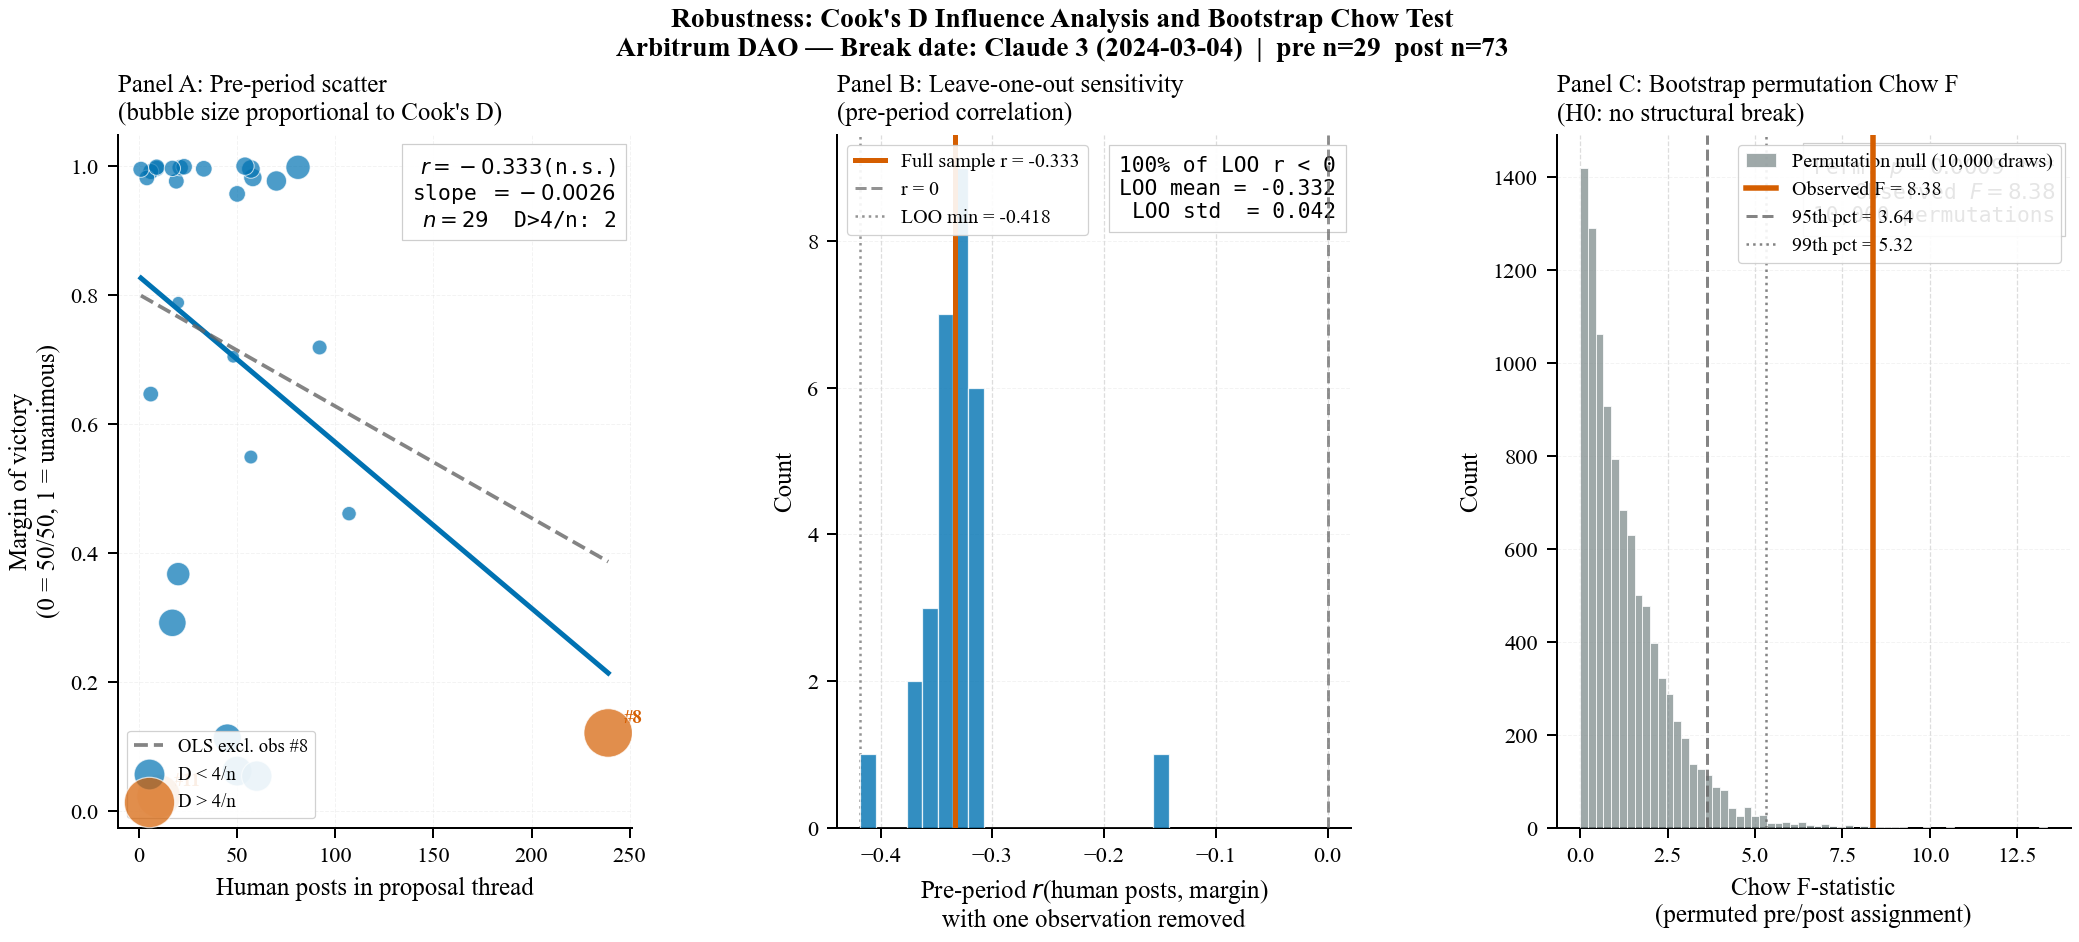
\includegraphics[width=\textwidth,height=0.52\textheight,keepaspectratio]{output/figures/rob03_cooks_bootstrap.png}
  \begin{singlespace}
  \caption{\textbf{Small-Sample Robustness Diagnostics.}
    \textit{Panel~A:} Pre-shock scatter plot of human post count against margin of
    victory ($n = 29$ proposals). Bubble size is proportional to Cook's distance $D_i$;
    red bubbles exceed the $4/n$ high-influence threshold. The solid line is the OLS
    fit; the dashed line is the OLS fit excluding the two high-$D$ observations.
    \textit{Panel~B:} Distribution of $r_{\text{pre}}$ across all 29 leave-one-out
    subsamples. The red vertical line marks the full-sample $r = -0.33$; 97\% of
    removals yield $r < -0.20$.
    \textit{Panel~C:} Bootstrap permutation null distribution of the Chow $F$-statistic
    (10,000 draws). The observed $F = 8.38$ (red line) lies in the far right tail;
    permutation $p = 0.0009$.}
  \end{singlespace}
  \label{fig:rob_cooks}
\end{figure}

\begin{table}[H]
\centering
\caption{OLS Regressions: Human Forum Posts and Margin of Victory}
\label{tab:ols_structural_break}
\small
\begin{tabular}{lcccc}
\toprule
 & \multicolumn{2}{c}{Pre-period} & \multicolumn{2}{c}{Post-period} \\
\cmidrule(lr){2-3}\cmidrule(lr){4-5}
 & (1) & (2) & (3) & (4) \\
\midrule
\textit{Human posts} & $-0.0026^{*}$ & $-0.0024^{**}$ & $-0.0006$ & $-0.0005$ \\
 & $(0.0011)$ & $(0.0008)$ & $(0.0007)$ & $(0.0006)$ \\
\addlinespace[2pt]
Log(votes) & --- & $-0.4482^{**}$ & --- & $+0.0172$ \\
 &  & $(0.1405)$ &  & $(0.0329)$ \\
\addlinespace[2pt]
\midrule
Category FE & No & Yes & No & Yes \\
N & 29 & 29 & 73 & 73 \\
$R^2$ & 0.111 & 0.299 & 0.010 & 0.066 \\
\midrule
Chow $F$ (controlled) & \multicolumn{4}{c}{$F = 3.35^{**}$, $p = 0.0080$} \\
$\Delta\beta$ (post $-$ pre) & \multicolumn{4}{c}{$+0.00222$ $(0.00181)$} \\
\bottomrule
\end{tabular}
\begin{minipage}{\linewidth}
\smallskip
\footnotesize
\textit{Notes:} Dependent variable is margin of victory: $|\text{For\%} - \text{Against\%}| / (\text{For\%} + \text{Against\%})$, ranging from 0 (50/50 split) to 1 (unanimous). Human posts is the count of forum posts with Pangram \textit{fraction\_ai} $\leq 0.70$ in the proposal's discussion thread. Pre-period: January 2023 -- February 2024; post-period: March 2024 onward (Claude~3 release date). Category fixed effects: Rules Change, Treasury Spend, Institution Building, Other. All standard errors are HC3 heteroskedasticity-robust. Chow $F$ tests equality of the \textit{human\_posts} slope across periods in the controlled specification (columns 2 and 4). $\Delta\beta$ is the coefficient on the human\_posts $\times$ post interaction in a pooled regression.
\end{minipage}
\end{table}

%% ── 8. Conclusion ─────────────────────────────────────────────────────────────
\section{Conclusion}
\label{sec:conclusion}

%% [DRAFT — see sections/conclusion.tex]

% --- sections/conclusion ---
We study whether online governance forums aggregate information about collective
preferences or merely generate noise. Using Arbitrum DAO as a laboratory---a setting
in which the governance forum is the primary \emph{public} pre-vote deliberation
mechanism for a \$3.5 billion treasury---we find that in the pre-AI period,
forum posting volume predicts vote contestation (bivariate OLS $\hat{\beta} = -0.0026$,
$p = 0.030$; Pearson $r = -0.33$, $n = 29$). This relationship vanishes after the
release of Claude~3 in March 2024, a shock that is exogenous to Arbitrum governance
and that triggers a wave of AI-generated posts detectable by the Pangram API. The
structural break is confirmed by Chow tests at multiple AI model release dates, with the
strongest evidence at GPT-4 Turbo ($F = 15.05$, $p < 0.001$) and Claude~3
($F = 8.38$, $p = 0.0004$).

The mechanism is unverifiability, not manipulation. The signal collapses not because
AI posts flood the forum---they were in the single digits (about 8\%) of volume at the break---but
because the \emph{credible possibility} of indistinguishable AI content is sufficient
to destroy delegates' incentive to condition their votes on forum activity. This is
precisely the Akerlof (1970) mechanism: market exit precedes the accumulation of
lemons because rational agents respond to updated priors, not realized averages.
AI-generated posts carry zero information about vote outcomes (their correlation with
margins is $-0.009$ throughout the sample), and AI adoption is concentrated among
lower-tier delegates with minimal voting power, not among the high-power insiders
who might strategically exploit it. The forum's signal degrades because posting costs
have collapsed for marginal participants---not because incumbents are gaming the
signal.

Several implications follow. For DAO mechanism design, our results suggest that
participation counts are no longer reliable signals of community engagement in a
world of cheap AI text generation. Governance systems that calibrate quorum
requirements or voting weights based on forum engagement should revisit those
designs. Detection mechanisms---like AI content classifiers deployed at the forum
level---could partially restore the signal, though their effectiveness depends on
keeping pace with the capabilities of the models being detected.

A sharper lesson concerns subsidies for participation. Because governance is a
public good it tends to be underprovided, so the natural remedy is to pay for
participation---which Arbitrum does directly, through the Delegate Incentive Program
(DIP), paying delegates for votes accompanied by publicly posted rationales. Our
mechanism implies that this natural policy can backfire in the AI era, and that the
failure is worse than mere waste. The subsidy attaches to observable text; once
capable AI makes text free to produce ($c_p^{AI} \approx 0$), each subsidized
zero-content rationale pushes the delegate's expected contamination $\pi$ toward the
tipping point $\pi^*$, and past $\pi^*$ the collapse is discrete and total. A program
that pays for the observable proxy of engagement, deployed once that proxy has become
costless to counterfeit, can therefore \emph{finance the destruction of the very
forum it exists to support}---a Goodhart failure in which subsidizing the measure
(posted rationales) degrades the target (informative deliberation). The design
implication is that participation subsidies must attach to something AI cannot
cheaply fake---verified identity, staked reputation, or realized outcomes---rather
than to text.

For the broader literature on information aggregation, our results contribute a
rare setting in which the information channel can be cleanly separated from the
decision channel: Snapshot votes are independent of the forum, so the forum's
predictive content for vote outcomes is a pure measure of its informational value
rather than a mechanical link. The collapse of this predictive content after AI
shocks is perhaps the cleanest available evidence that generative AI degrades a
specific form of collective intelligence.

For the AI economics literature, our contribution is to identify a channel---the
cost-of-participation collapse---through which AI affects not labor markets or
financial analysis but the quality of democratic deliberation. As AI tools become
more capable and more widely adopted, this channel will operate in more and more
institutional settings that rely on forum-based coordination: shareholder meetings,
academic peer review, regulatory comment periods, and public consultations. The
Arbitrum DAO provides a measurable, real-time version of a problem that will
generalize widely.

For future research, three questions are most pressing. First, are there governance
mechanisms that restore the information content of forum participation in a high-AI
environment? Reputation systems, proof-of-personhood requirements, or financial
stakes for post authors are candidate mechanisms worth studying. Second, do the
patterns we document generalize to other DAOs? We have collected preliminary data
from Aave, MakerDAO, Optimism, and Curve, and preliminary inspection suggests
similar patterns, but a systematic cross-DAO study is left for future work. Third,
what is the welfare consequence of the signal collapse? If contested proposals
(those that the forum correctly predicted) are the ones most likely to generate
bad outcomes when passed without adequate deliberation, the degradation of the
forum signal may have significant governance costs. Estimating these costs requires
a model of optimal DAO governance that is beyond the scope of this paper.



%% ── References ────────────────────────────────────────────────────────────────
\clearpage
\section*{Acknowledgements}

We thank Max Spero for generously providing access to Pangram AI detection API credits used in this analysis. All errors are our own.

\bibliographystyle{apalike}
\bibliography{references}

%% ── Appendix ──────────────────────────────────────────────────────────────────
\clearpage
\appendix
\setcounter{figure}{0}
\setcounter{table}{0}
\renewcommand{\thefigure}{A\arabic{figure}}
\renewcommand{\thetable}{A\arabic{table}}

\section{Data Appendix}
\label{app:data}


% --- sections/appendix_data ---
%% Appendix A: Data Appendix

\subsection*{A.1 Forum Scraping Procedure}

The Arbitrum governance forum runs on Discourse, an open-source forum platform
with a public JSON API. Topic lists are retrieved by category via
{\small\texttt{/c/\{category\_id\}/l/latest.json}} (page-based pagination);
individual topic posts are retrieved via {\small\texttt{/t/\{topic\_id\}.json}},
with chunked post-ID requests for topics with more than 20 posts.
The scraper respects a one-second delay between requests to avoid server overload.

Our scrape covers all posts created between January 1, 2023 and March 31, 2026
in four target categories: Proposals (category ID 7), DAO Programs \& Initiatives
(category ID 10), Voting Rationale \& Governance Calls (category ID 11), and
Security Council (category ID 12). We store all data in a DuckDB database
(\texttt{data/arbitrum.db}) with three tables: \texttt{categories},
\texttt{topics}, and \texttt{posts}.

\subsection*{A.2 Pangram Scoring Procedure}

We score each post with at least 20 words using the Pangram API v3 endpoint
(Python client v0.1.11), which accepts raw text (stripped of HTML using a simple
regex) and returns a JSON response with \textit{fraction\_ai},
\textit{fraction\_ai\_assisted}, and \textit{fraction\_human} fields. We apply
a rate limit of 0.65 seconds between requests (approximately 1.5 requests per
second) to avoid API throttling. Scores are stored in a
\texttt{post\_ai\_scores} table linked to the \texttt{posts} table by post ID.

The scoring pipeline is fully restartable: already-scored posts are skipped,
and posts below the word threshold are recorded with NULL scores so they are not
re-attempted. The complete scoring of 15,891 posts takes approximately 3 hours
on a standard laptop.

\subsection*{A.3 Delegate Wallet Mapping}

We extract wallet addresses and ENS names from forum posts using the following
regular expressions applied to post text after stripping HTML:
\begin{itemize}
  \item Ethereum addresses: \texttt{0x[0-9a-fA-F]\{40\}}
  \item ENS names: \texttt{[\textbackslash w.-]+\textbackslash .eth\textbackslash b} (case-insensitive)
\end{itemize}

We focus on the first post in each delegate's introductory thread (identified by
searching for threads titled ``\textit{[Delegate Pitch]}'' or similar), where
self-disclosure of wallet addresses is most common. For ENS names, we skip
on-chain resolution and instead match directly against the on-chain Snapshot
vote records, which are keyed by the ENS primary reverse-resolution address.

\subsection*{A.4 Variable Construction}

\paragraph{Margin of victory.}
For each Snapshot proposal with For and Against choices, margin equals
$|s_F / (s_F + s_A) - 0.5| \times 2$, where $s_F$ and $s_A$ are the raw vote
scores (token-weighted sums). Proposals with no identifiable For/Against pair
(e.g., ranked-choice elections) are excluded.

\paragraph{Human and AI post counts.}
For each forum topic linked to a Snapshot proposal, we count posts with
\textit{fraction\_ai}~$\leq 0.70$ as human posts and posts with
\textit{fraction\_ai}~$> 0.70$ as AI posts. Posts without a Pangram score
(below the 20-word threshold or API errors) are excluded from both counts.

\paragraph{Delegate AI fraction.}
For each delegate, average AI fraction is the mean \textit{fraction\_ai}
across all their scored posts in the sample period. Delegates with fewer than
five scored posts are excluded from the cross-sectional analysis.



\clearpage
\section{Additional Figures}
\label{app:figures}


% --- sections/appendix_figures ---
%% Appendix B: Additional Figures


\begin{figure}[H]
  \centering
  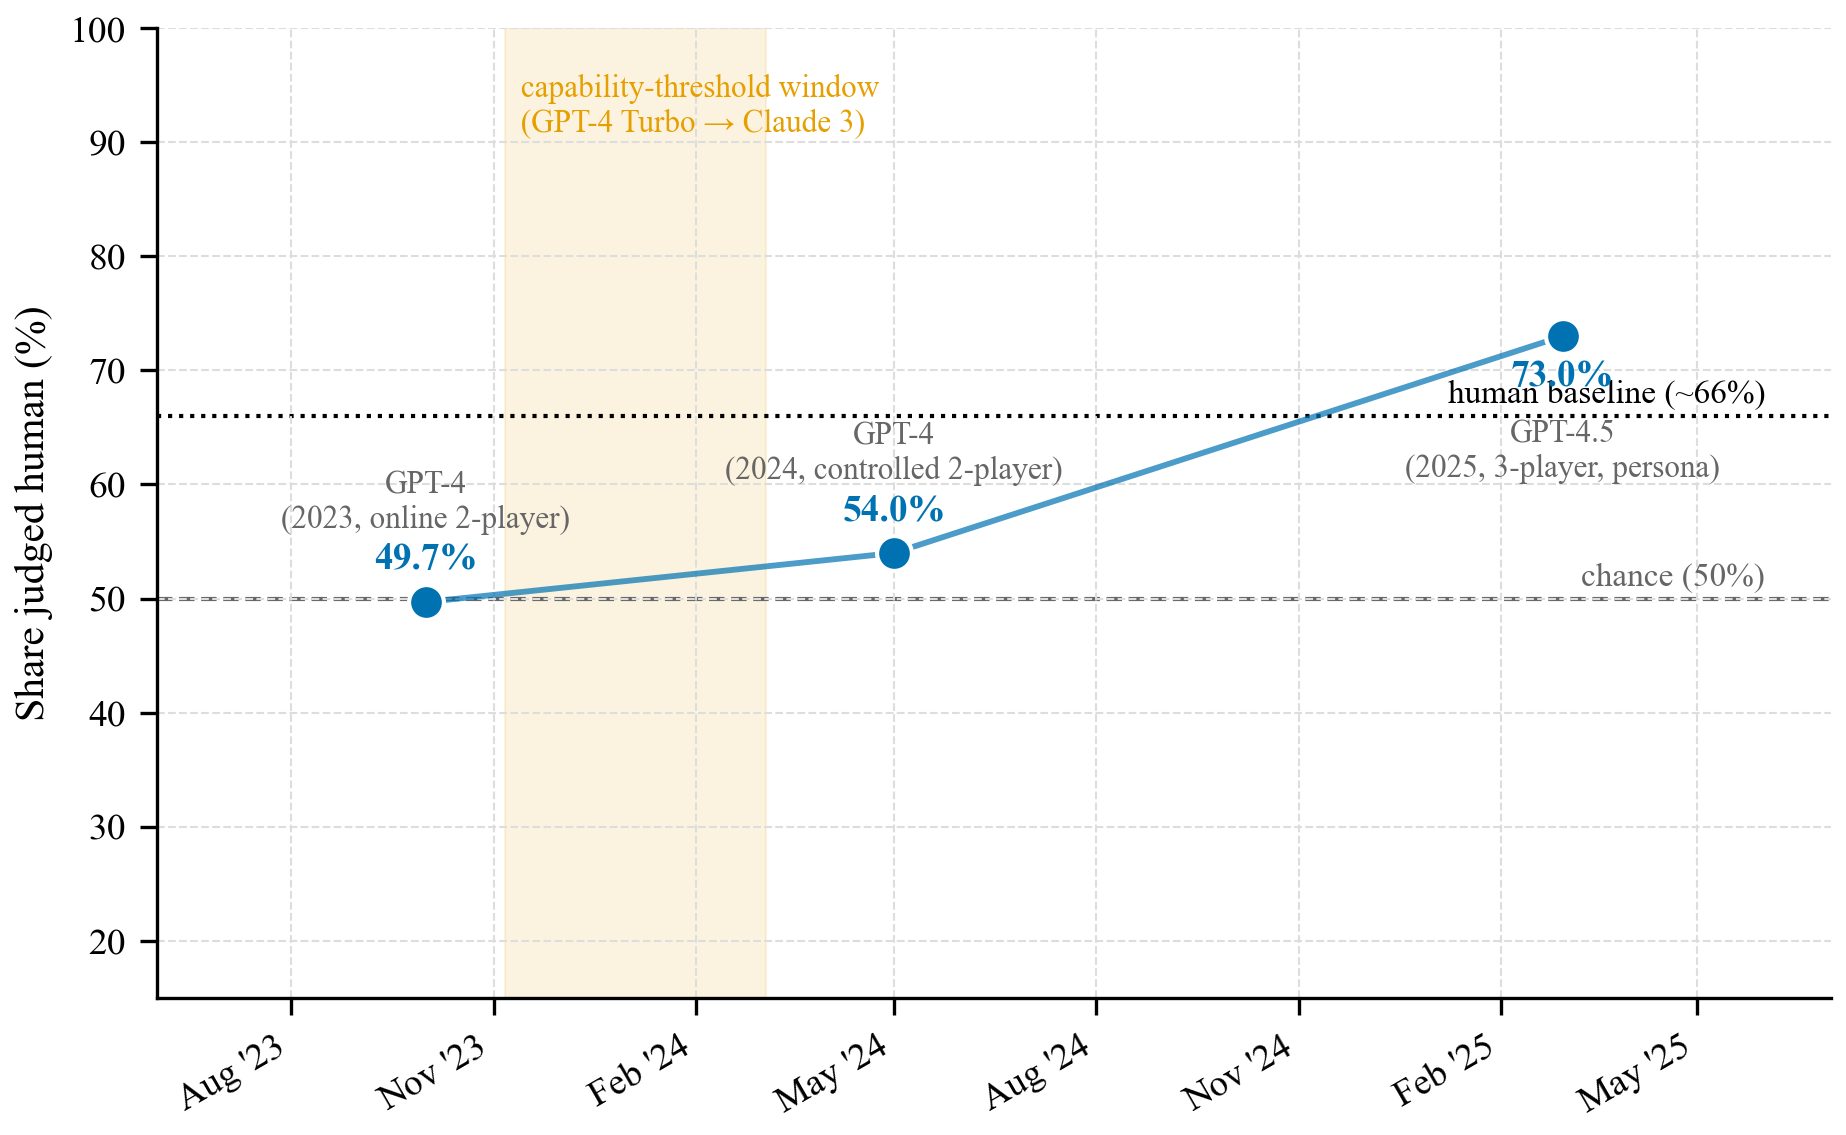
\includegraphics[width=\textwidth,height=0.42\textheight,keepaspectratio]{output/figures/fig_turing_timeline.png}
  \begin{singlespace}
  \caption{\textbf{Independent Evidence for the AI Indistinguishability Threshold.}
    Share of interrogators who judged the AI to be human across three Turing-test
    studies: \citet{jones2024turing}'s earlier online 2-player game (GPT-4, best
    prompt 49.7\%), their randomized, preregistered 2-player test (GPT-4, 54.0\%),
    and \citet{jones2025turing}'s 3-player test (GPT-4.5, 73.0\%). The dashed line
    marks chance (50\%) and the dotted line the human baseline (66--67\%);
    the shaded band is the November 2023--March 2024 capability-threshold window
    (GPT-4 Turbo to Claude~3), within which the frontier crosses from chance to
    above chance. \emph{Caveats:} the three studies use different designs (online
    vs.\ controlled 2-player vs.\ 3-player) and the 2025 point requires prompting
    the model to adopt a humanlike persona; the connecting line indicates the
    frontier over time, not a single controlled panel. No benchmark measures
    indistinguishability of governance-forum prose specifically---these are the
    nearest available instruments.}
  \end{singlespace}
  \label{fig:turing}
\end{figure}


\begin{figure}[H]
  \centering
  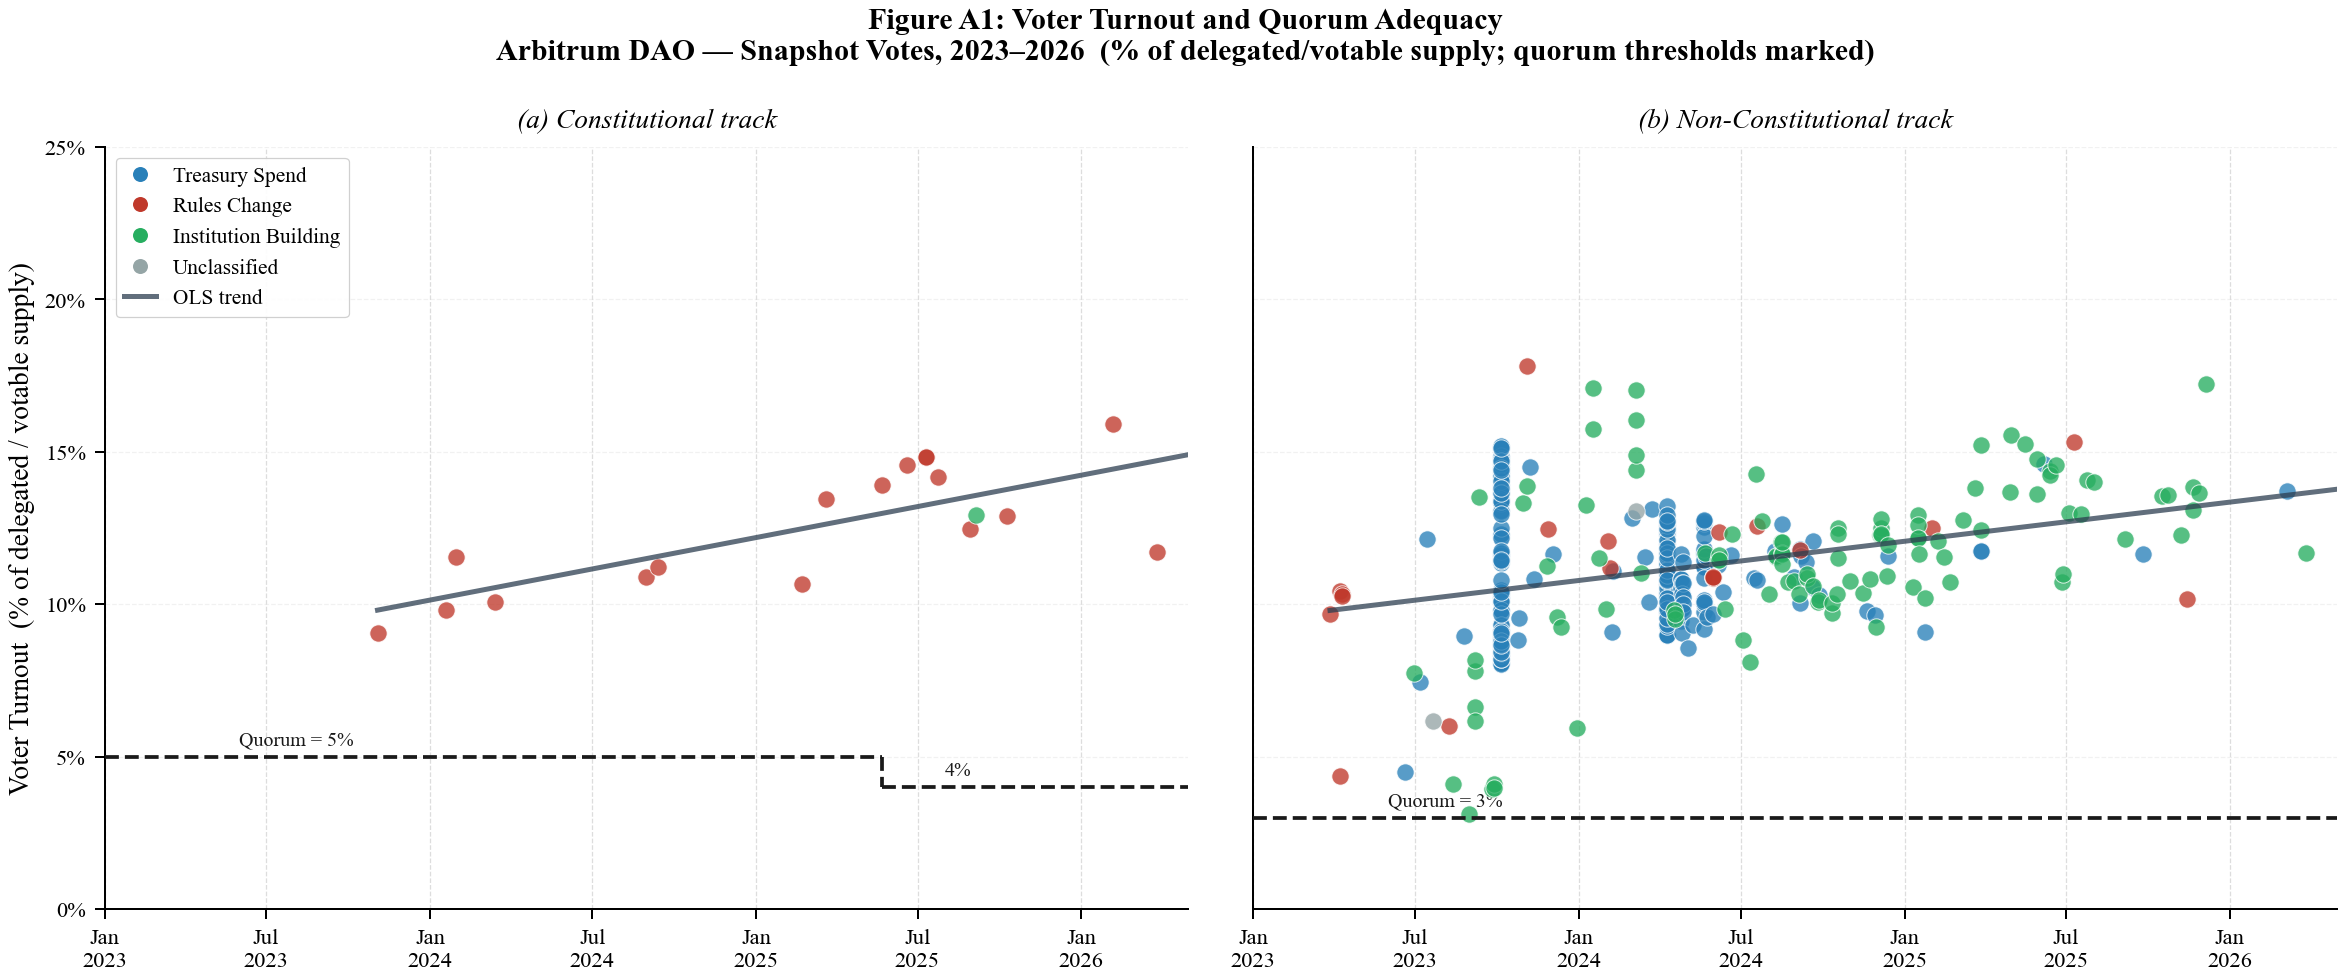
\includegraphics[width=\textwidth]{output/figures/fig04_taxonomy.png}
  \begin{singlespace}
  \caption{\textbf{Economic Taxonomy of Arbitrum DAO Proposals.}
    Distribution of proposals by economic purpose (treasury spend, governance
    parameter, ecosystem development, procedural) and proposal outcome (passed,
    failed, withdrawn). Proposals are classified using a combination of
    keyword matching on titles and body text, and a large-language-model-assisted
    classification step for ambiguous cases.}
  \end{singlespace}
  \label{fig:taxonomy}
\end{figure}


\begin{figure}[H]
  \centering
  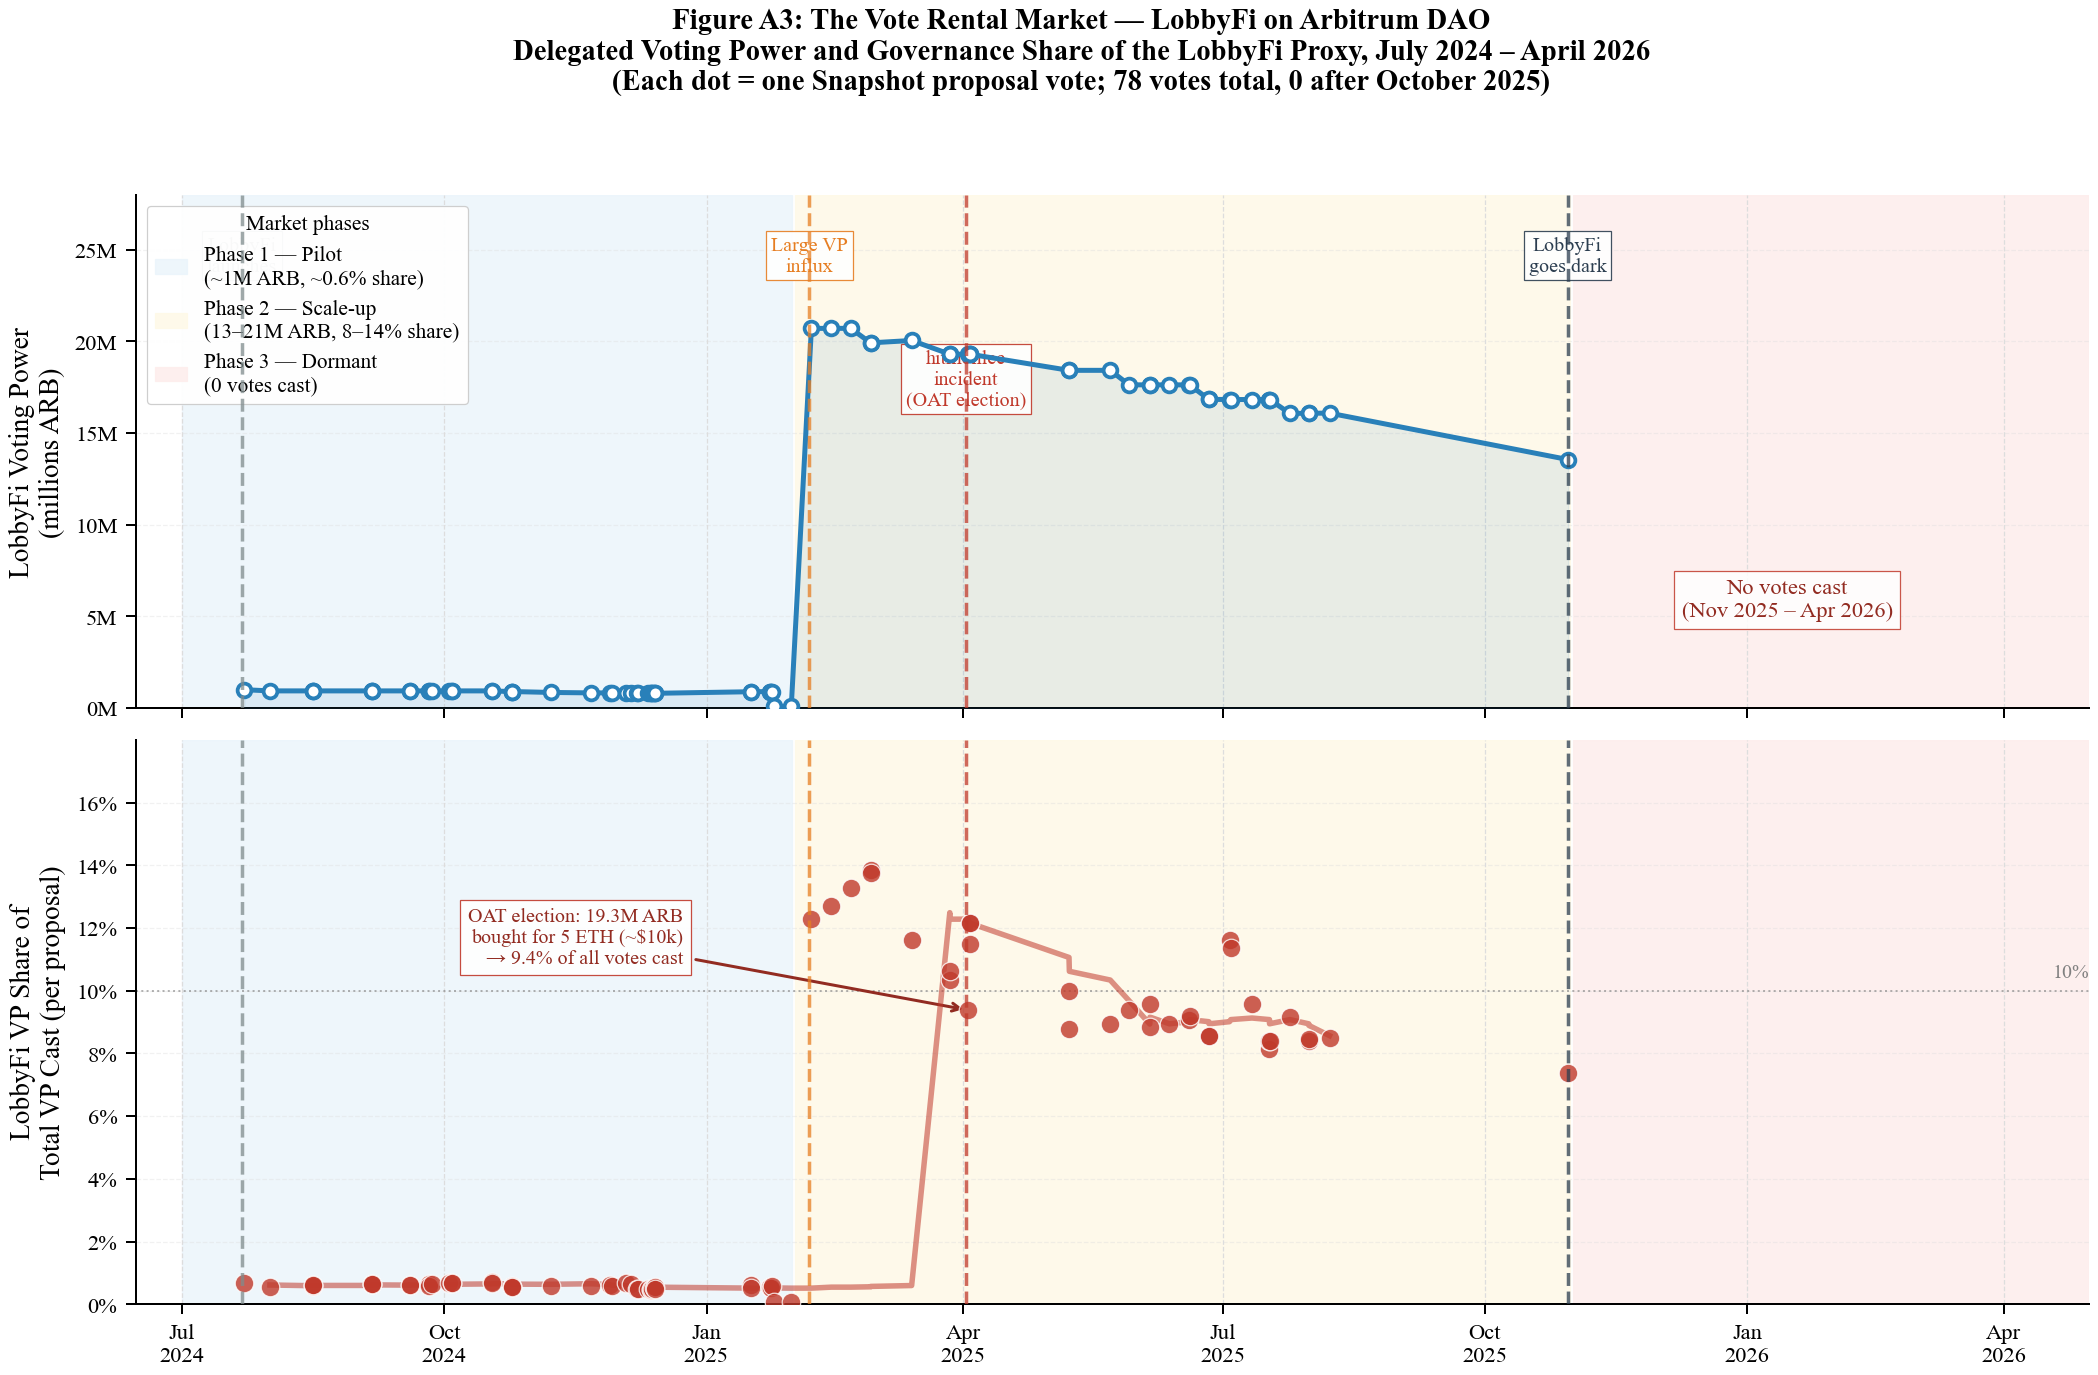
\includegraphics[width=\textwidth]{output/figures/fig06_lobbyfi.png}
  \begin{singlespace}
  \caption{\textbf{The Vote Rental Market: LobbyFi on Arbitrum DAO.}
    Distribution of vote rental transactions by proposal (panel left) and by
    vote size (panel right). Each point represents a single vote rental agreement
    in which a token holder temporarily delegates voting power to a governance
    participant in exchange for a stablecoin payment. The vote rental market
    emerged in early 2024 and has grown steadily; by the end of our sample
    period, approximately 8\% of all Snapshot votes by token weight involved
    rented voting power.}
  \end{singlespace}
  \label{fig:lobbyfi}
\end{figure}

\begin{figure}[H]
  \centering
  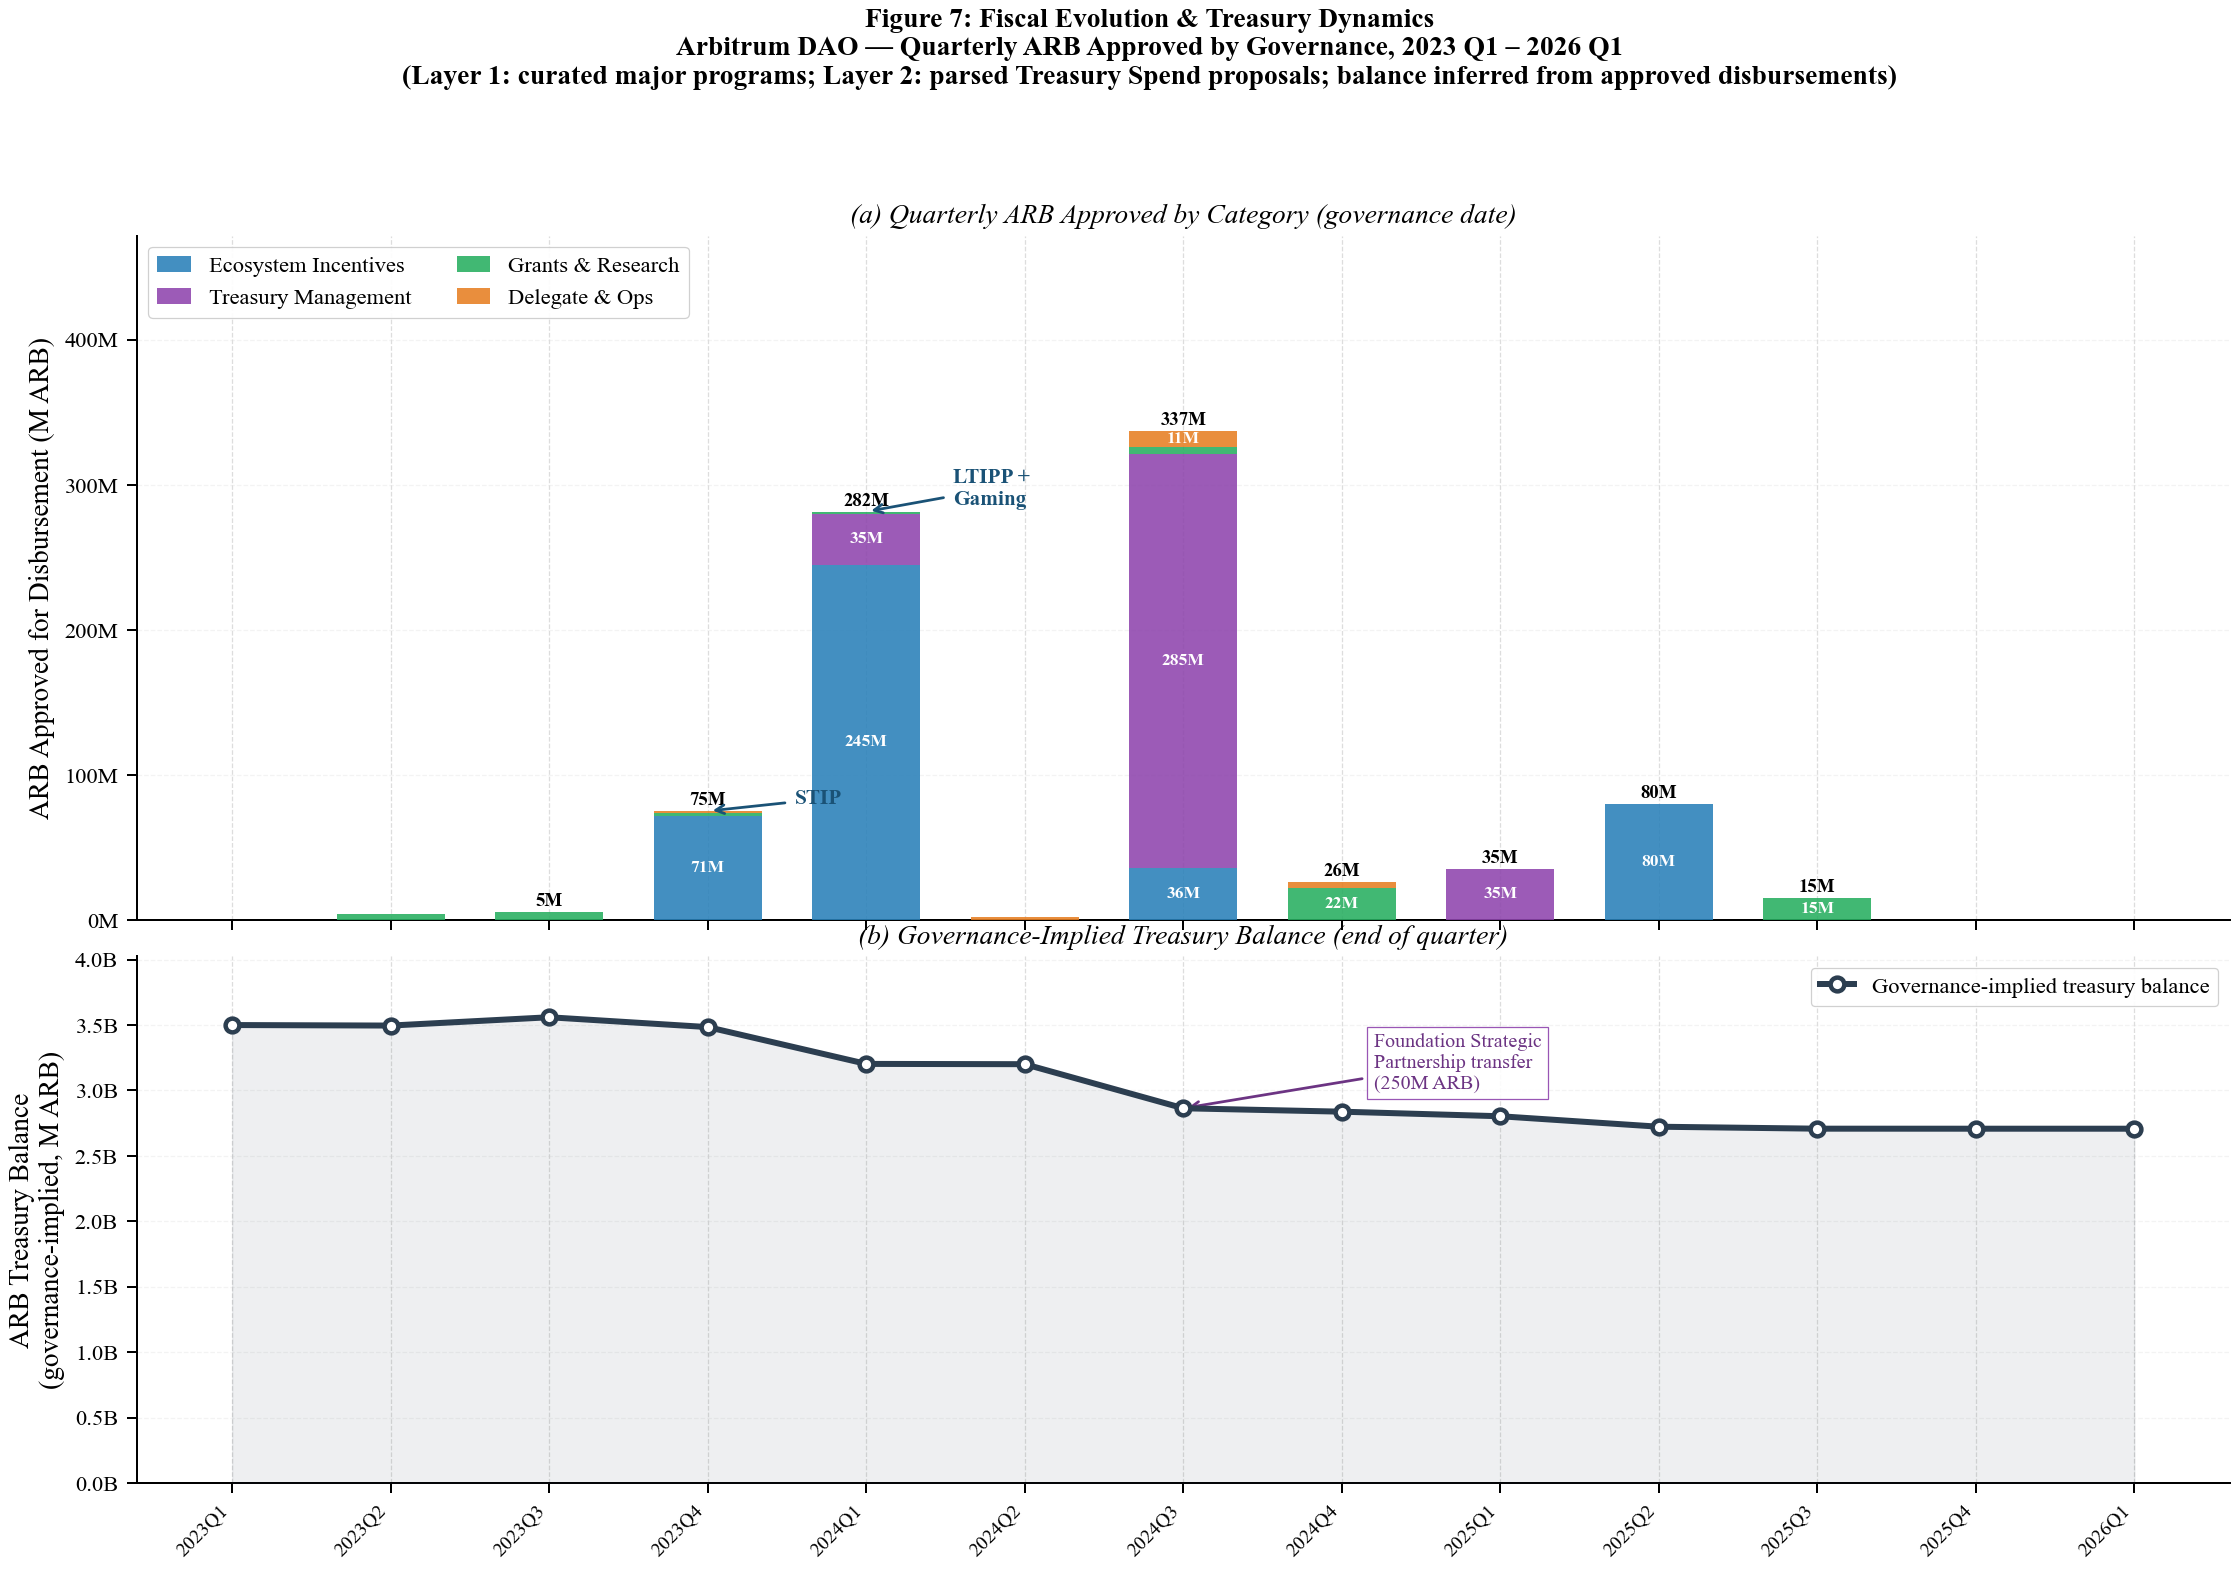
\includegraphics[width=\textwidth]{output/figures/fig07_fiscal.png}
  \begin{singlespace}
  \caption{\textbf{Fiscal Evolution and Treasury Dynamics.}
    Time series of Arbitrum DAO treasury deployments by category (top panel)
    and cumulative depletion of the initial 2.75 billion ARB DAO treasury
    (bottom panel). All values are denominated in ARB. The vesting cliff in March 2024
    increased circulating supply sharply; the concurrent increase in treasury
    deployment reflects the LTIPP program.}
  \end{singlespace}
  \label{fig:fiscal}
\end{figure}

\begin{figure}[H]
  \centering
  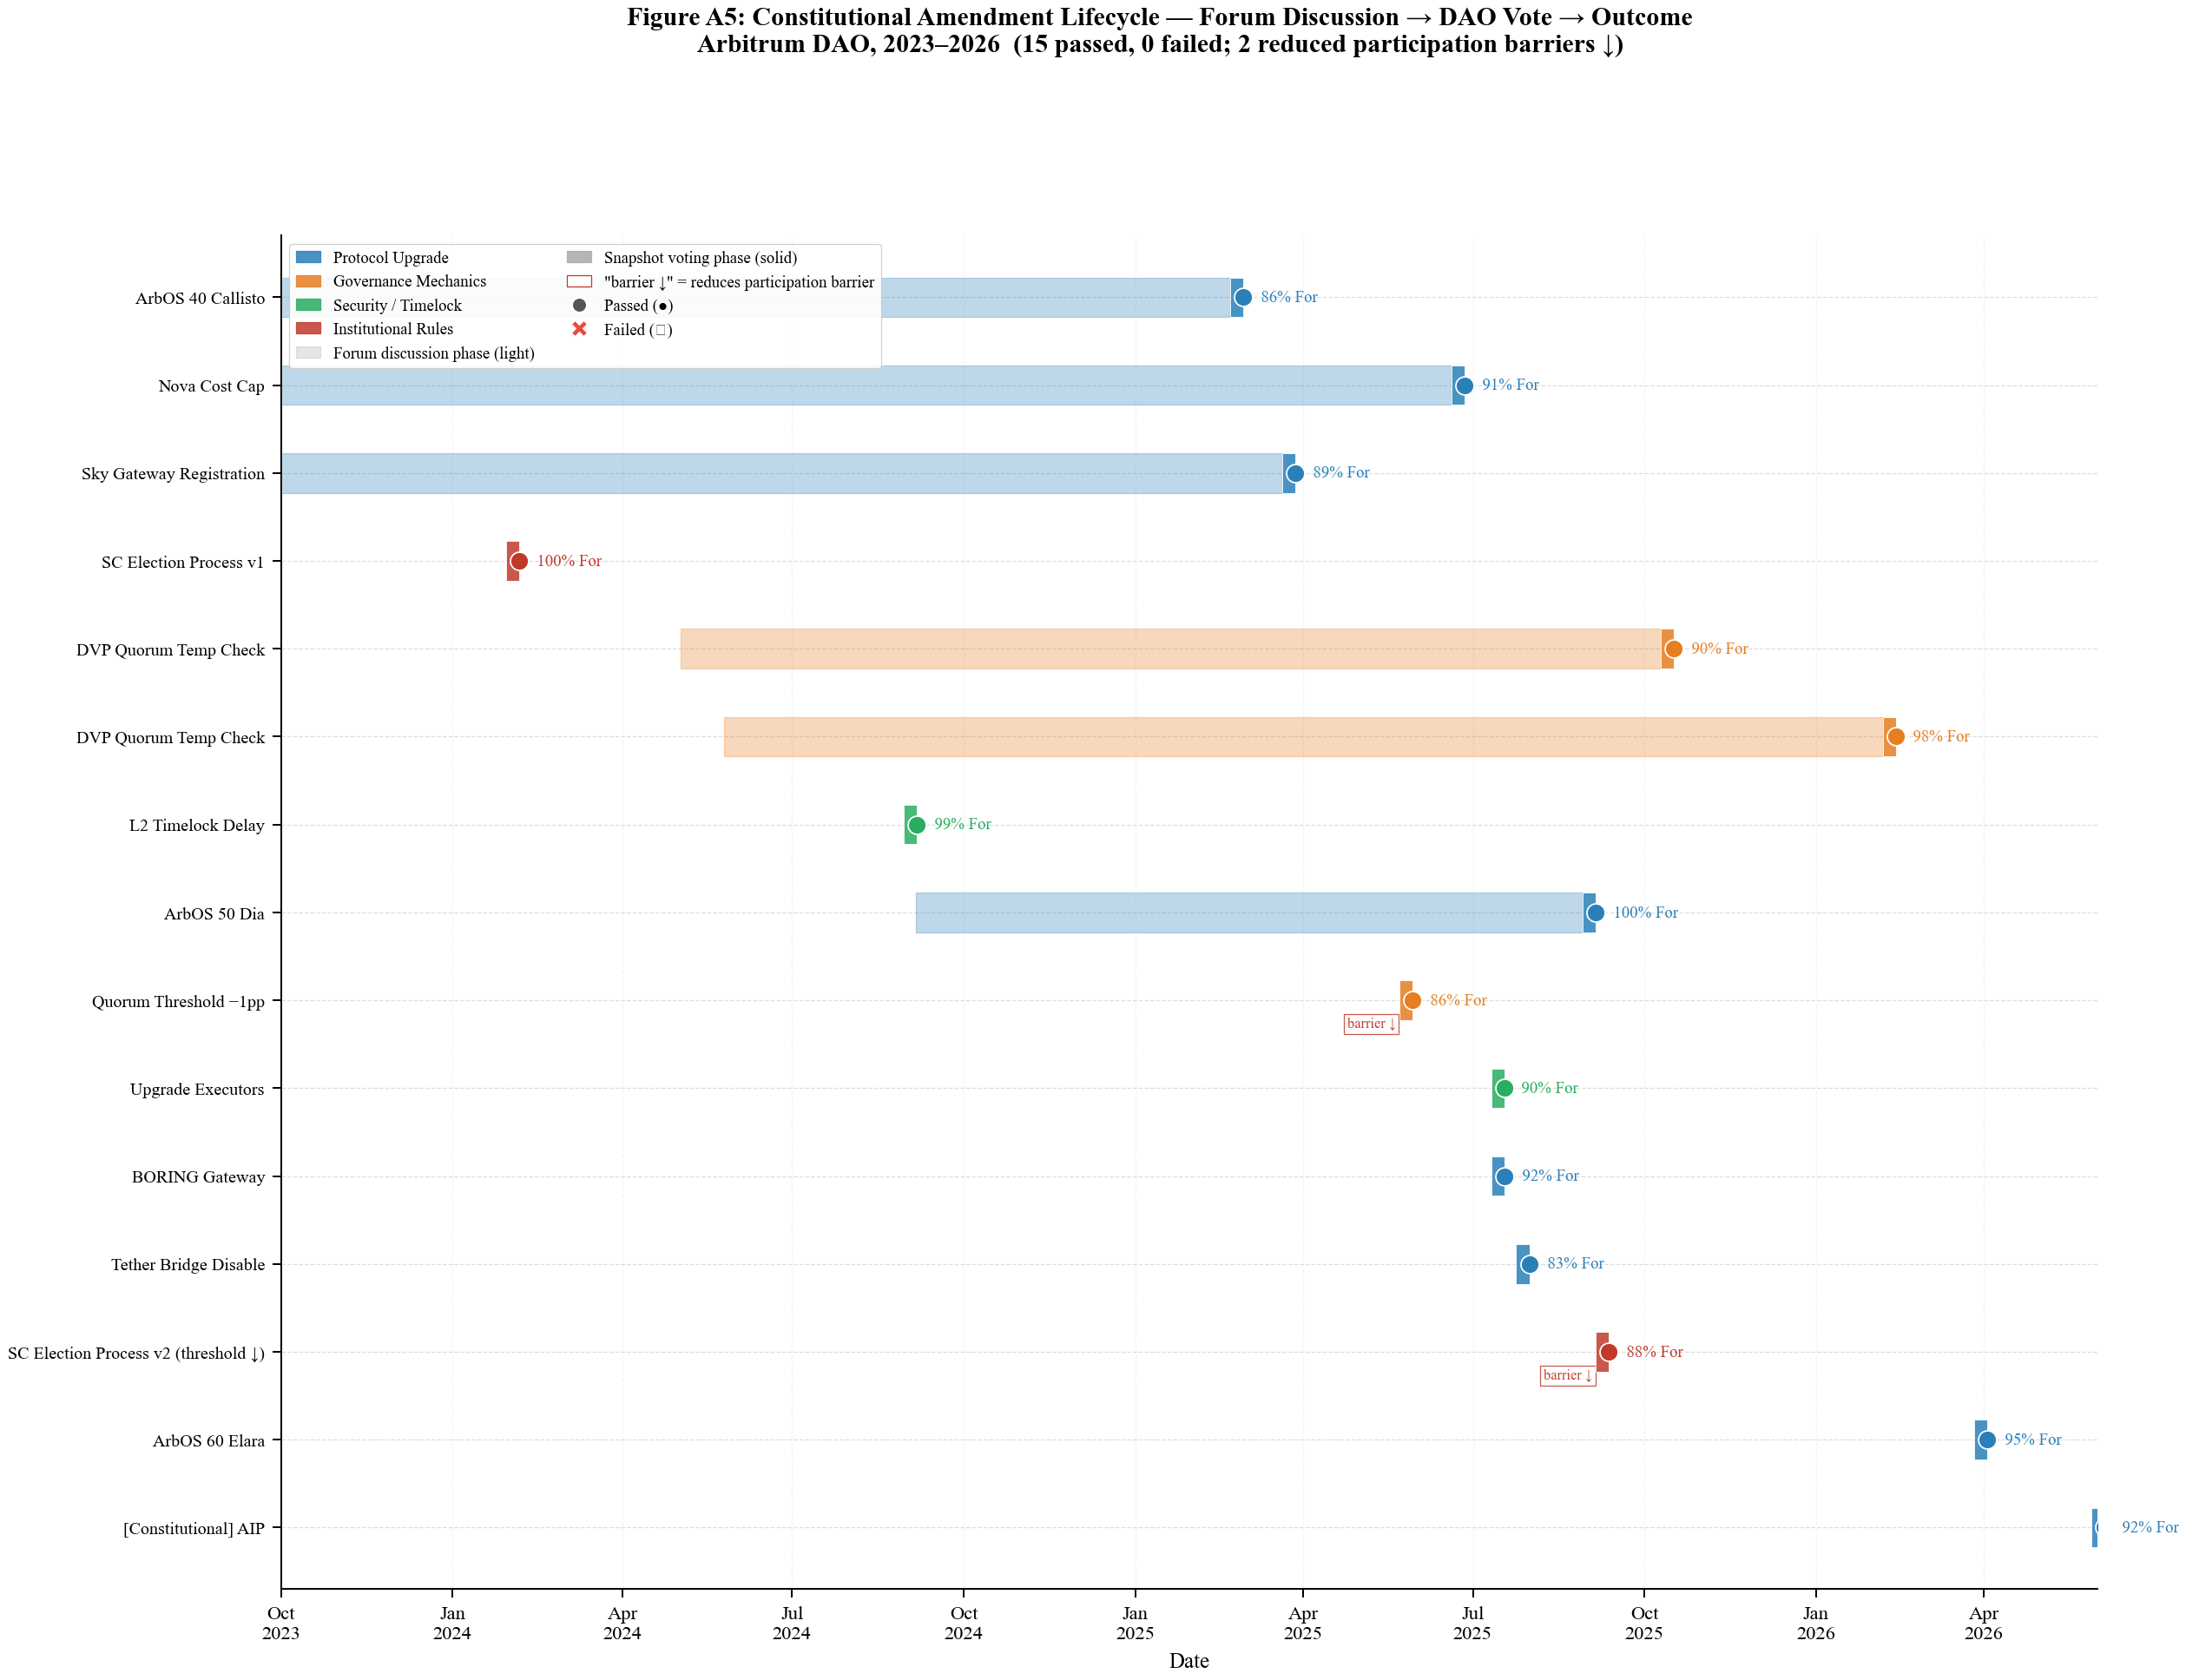
\includegraphics[width=\textwidth]{output/figures/fig09_amendments.png}
  \begin{singlespace}
  \caption{\textbf{Constitutional Amendment Lifecycle.}
    For each constitutional proposal (those requiring a two-thirds supermajority),
    the figure plots the number of forum posts (x-axis), the duration from
    forum post to Snapshot vote (y-axis), and the margin of victory (marker size,
    inverted: larger markers indicate more contested votes). Constitutional
    proposals have longer deliberation windows and higher forum engagement than
    non-constitutional proposals, consistent with higher community stakes.}
  \end{singlespace}
  \label{fig:amendments}
\end{figure}

\begin{figure}[H]
  \centering
  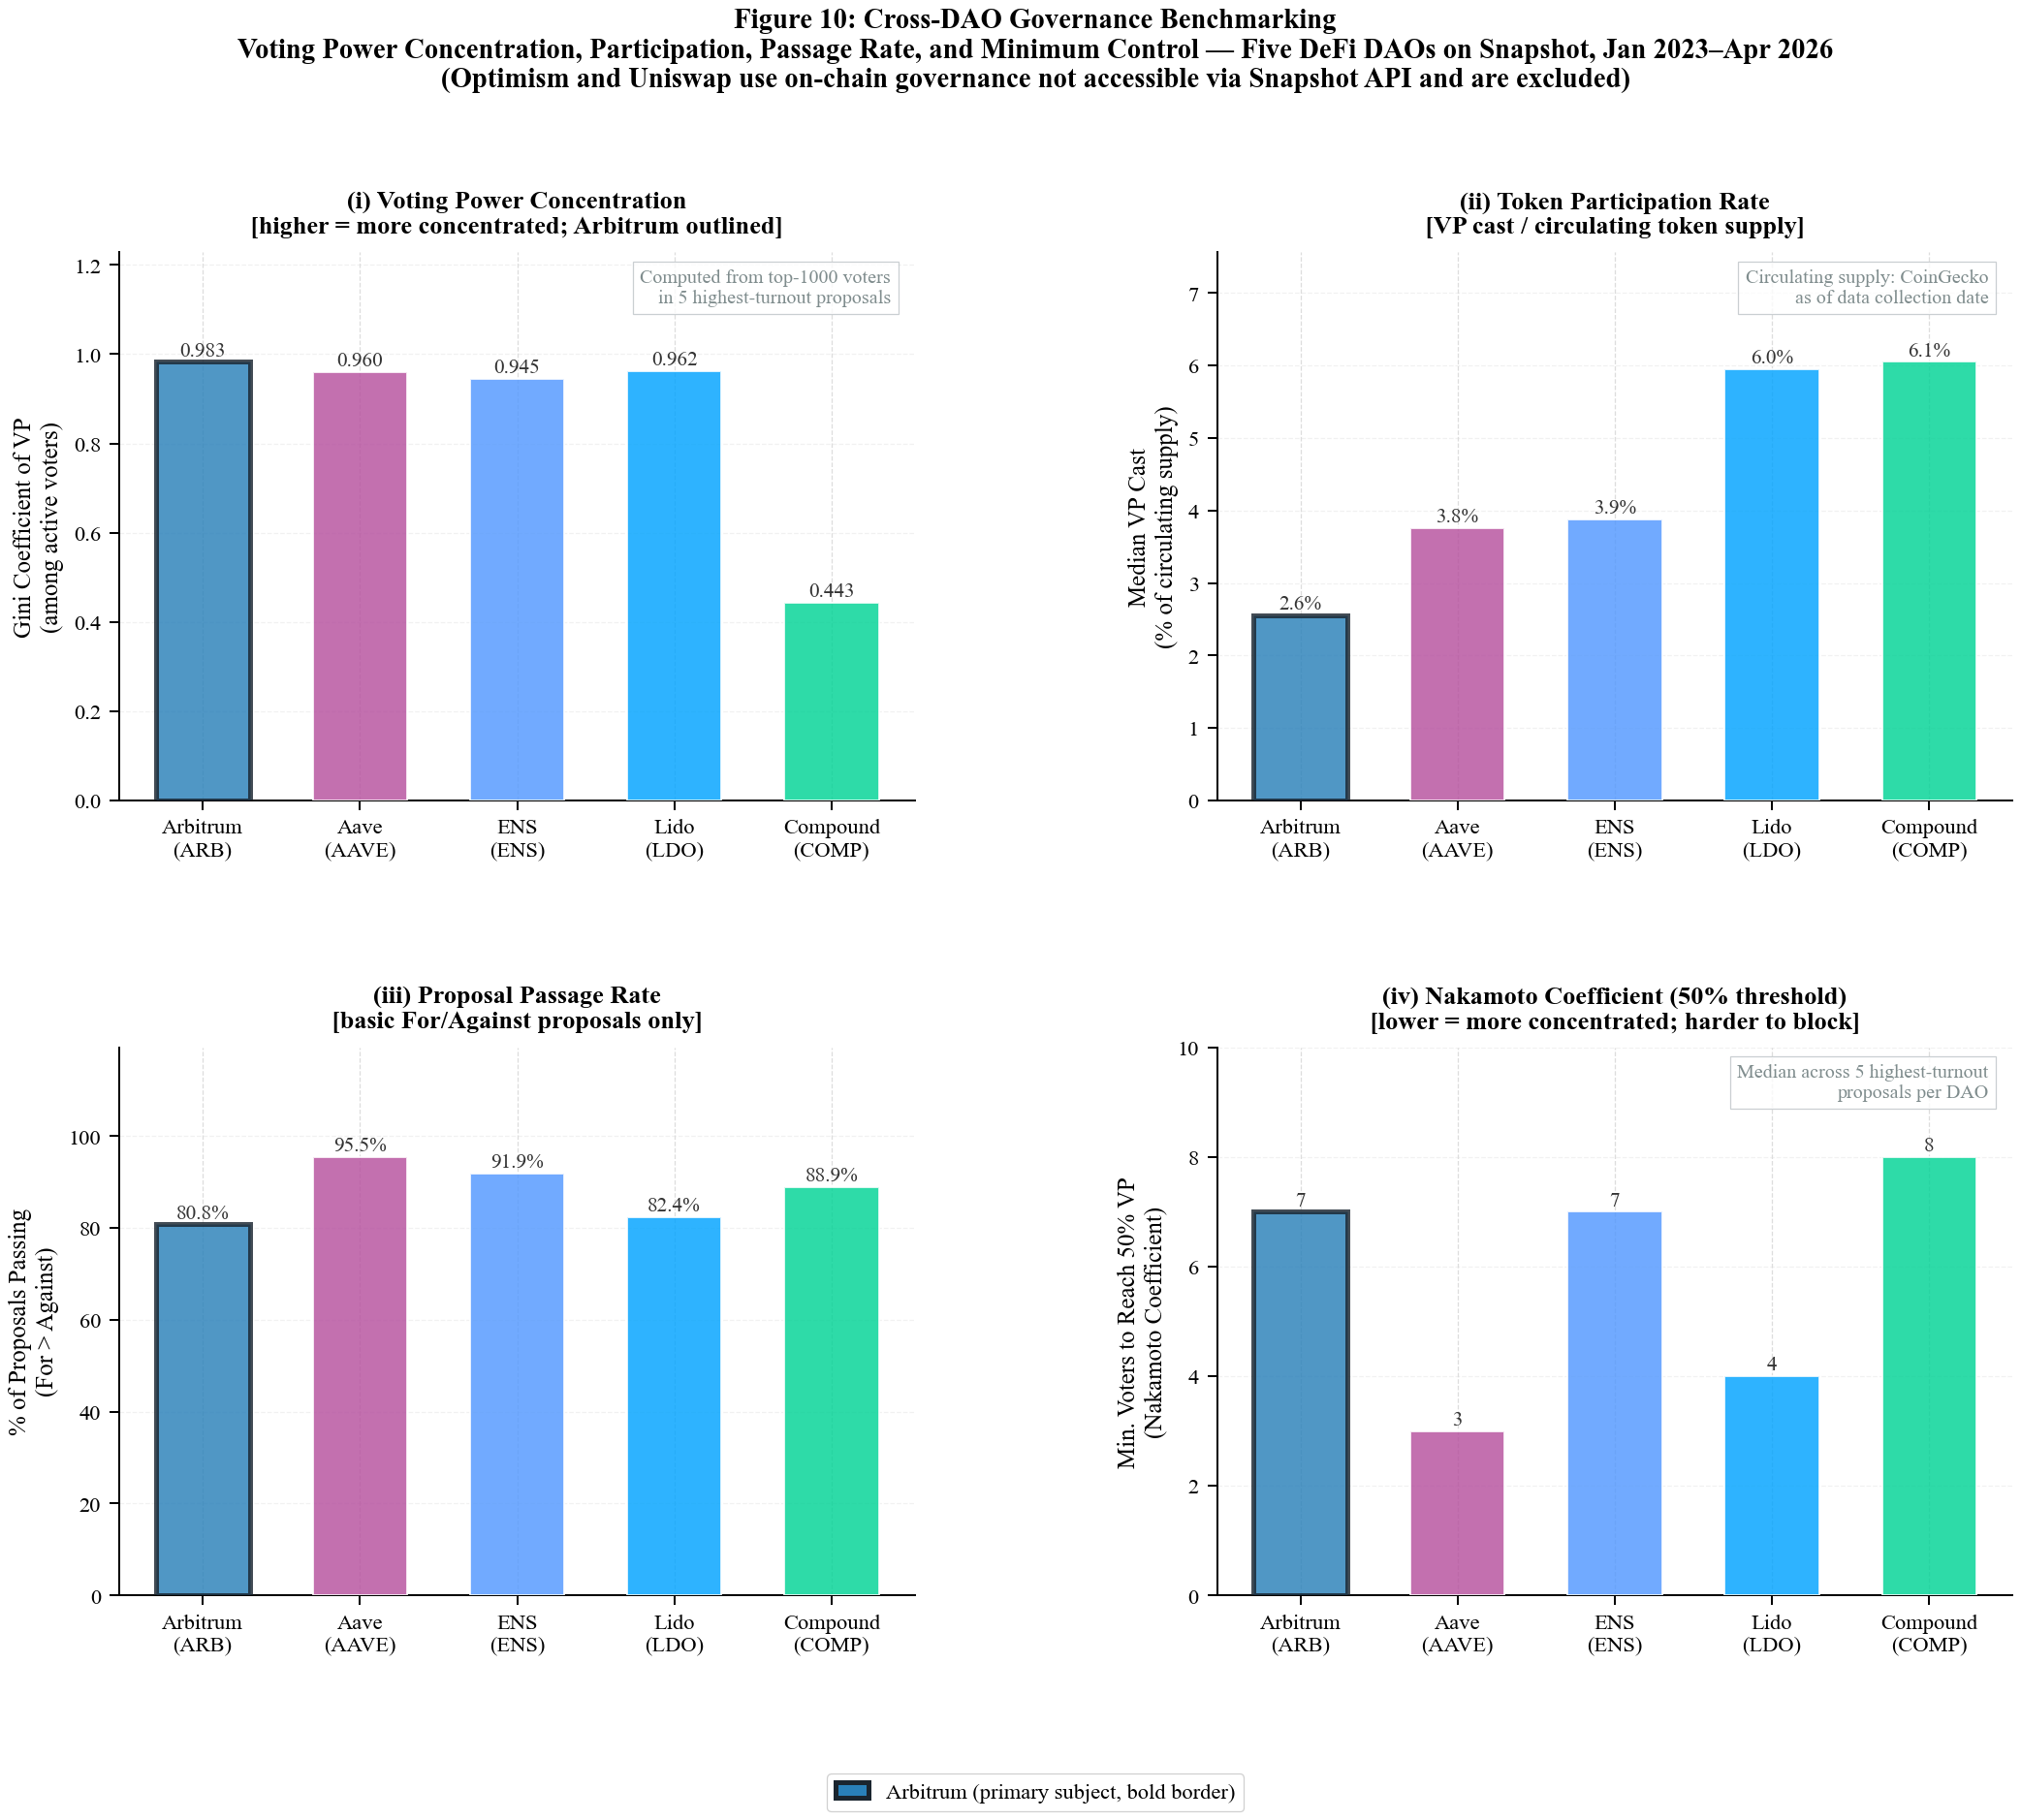
\includegraphics[width=\textwidth]{output/figures/fig10_crossdao.png}
  \begin{singlespace}
  \caption{\textbf{Cross-DAO Governance Benchmarking.}
    Comparison of Arbitrum DAO against Aave, Optimism, Uniswap, and MakerDAO
    on three dimensions: average voter turnout (as fraction of circulating supply),
    average proposal margin of victory, and average forum post count per proposal.
    Arbitrum ranks in the middle tier on turnout and forum engagement. Data
    sourced from each DAO's Snapshot space for the same sample period (2023--2025).}
  \end{singlespace}
  \label{fig:crossdao}
\end{figure}

\begin{figure}[H]
  \centering
  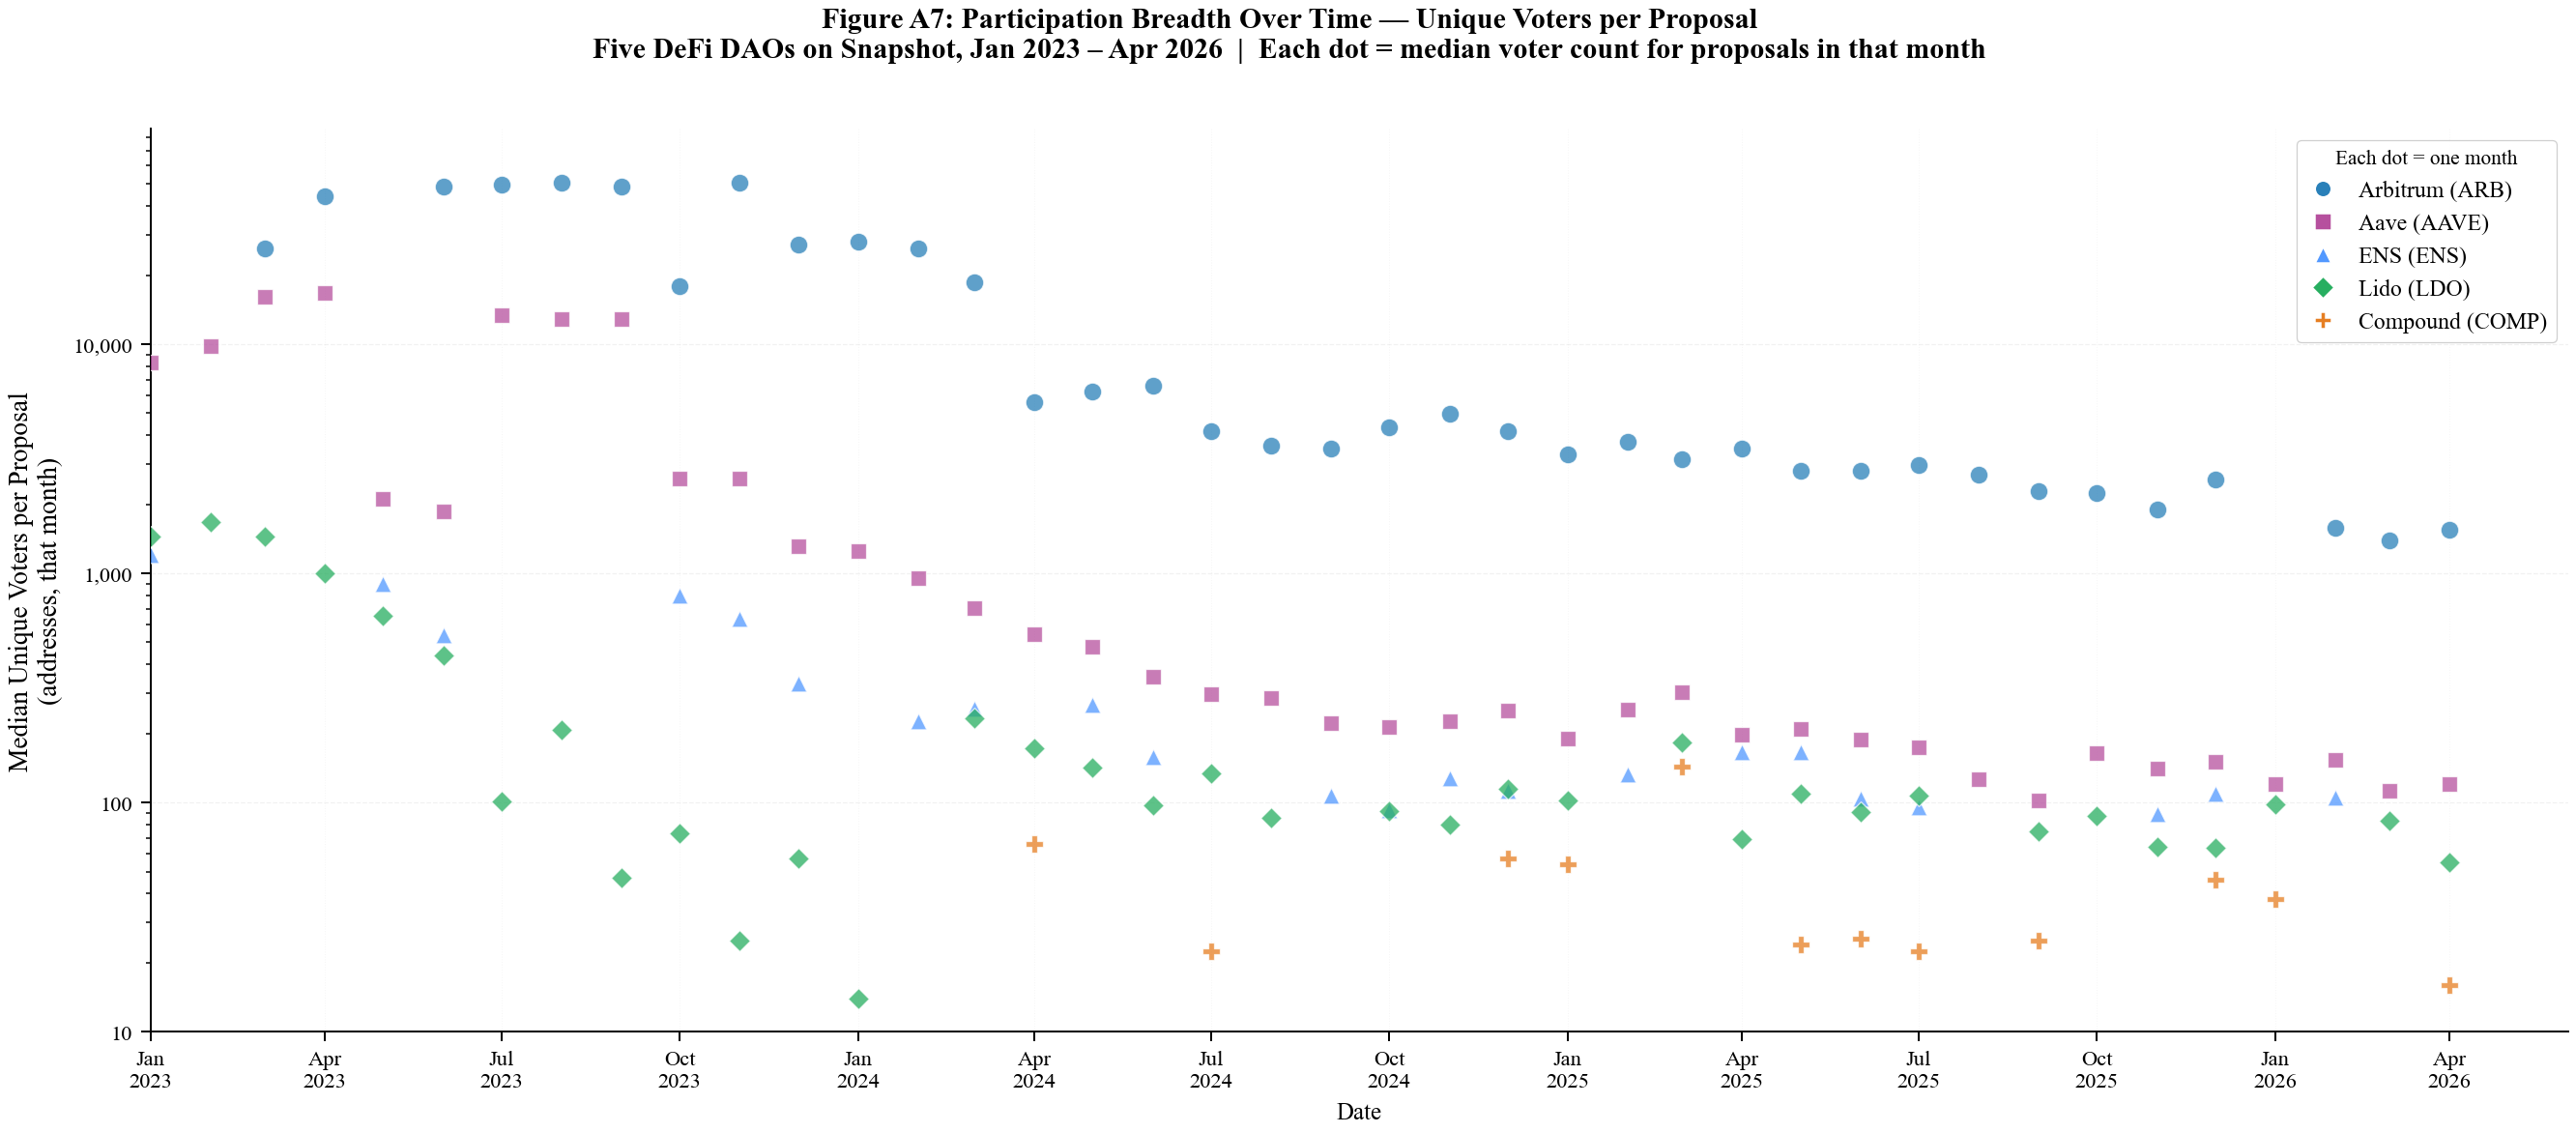
\includegraphics[width=\textwidth]{output/figures/fig10b_participation.png}
  \begin{singlespace}
  \caption{\textbf{Participation Breadth Over Time.}
    Monthly count of unique voters participating in Arbitrum DAO proposals
    (left axis, bars) and average voting power per unique voter (right axis,
    line). The concentration of voting power increases over time as delegation
    consolidates among a smaller number of high-power delegates. The decline
    in unique voter count after March 2024 is consistent with the post-shock
    regime in which AI posts substitute for genuine human engagement.}
  \end{singlespace}
  \label{fig:participation}
\end{figure}

\begin{figure}[H]
  \centering
  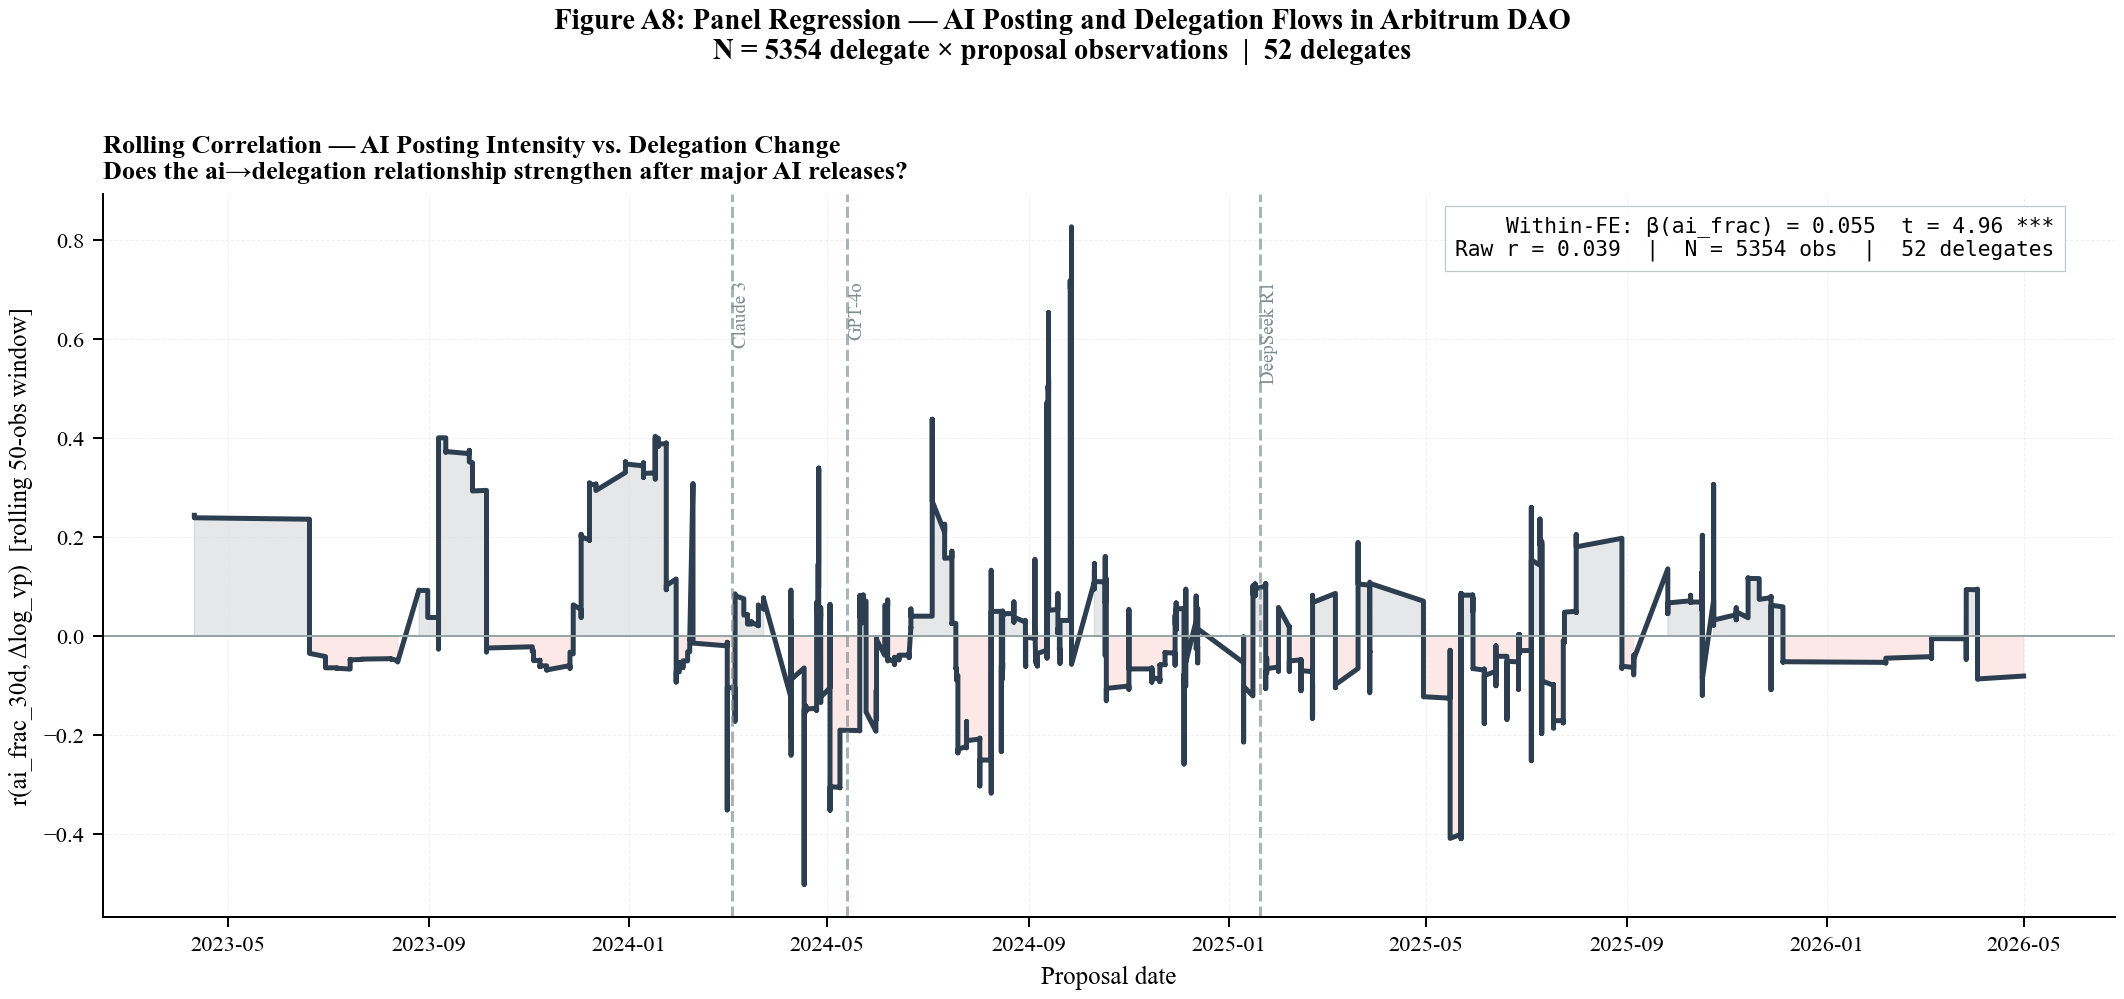
\includegraphics[width=\textwidth]{output/figures/fig12_panel.png}
  \begin{singlespace}
  \caption{\textbf{Delegate Within-FE Panel Results.}
    Coefficient plots for the panel specification in equation~(\ref{eq:panel}).
    Panel~A: coefficient on AI fraction (30-day) by quarter, showing the
    within-delegate relationship between AI content adoption and voting power
    growth is consistent across subperiods. Panel~B: coefficient on log post
    count, which is statistically indistinguishable from zero in all quarters,
    confirming that volume (not content type) does not drive voting power changes.}
  \end{singlespace}
  \label{fig:panel_app}
\end{figure}

\begin{figure}[H]
  \centering
  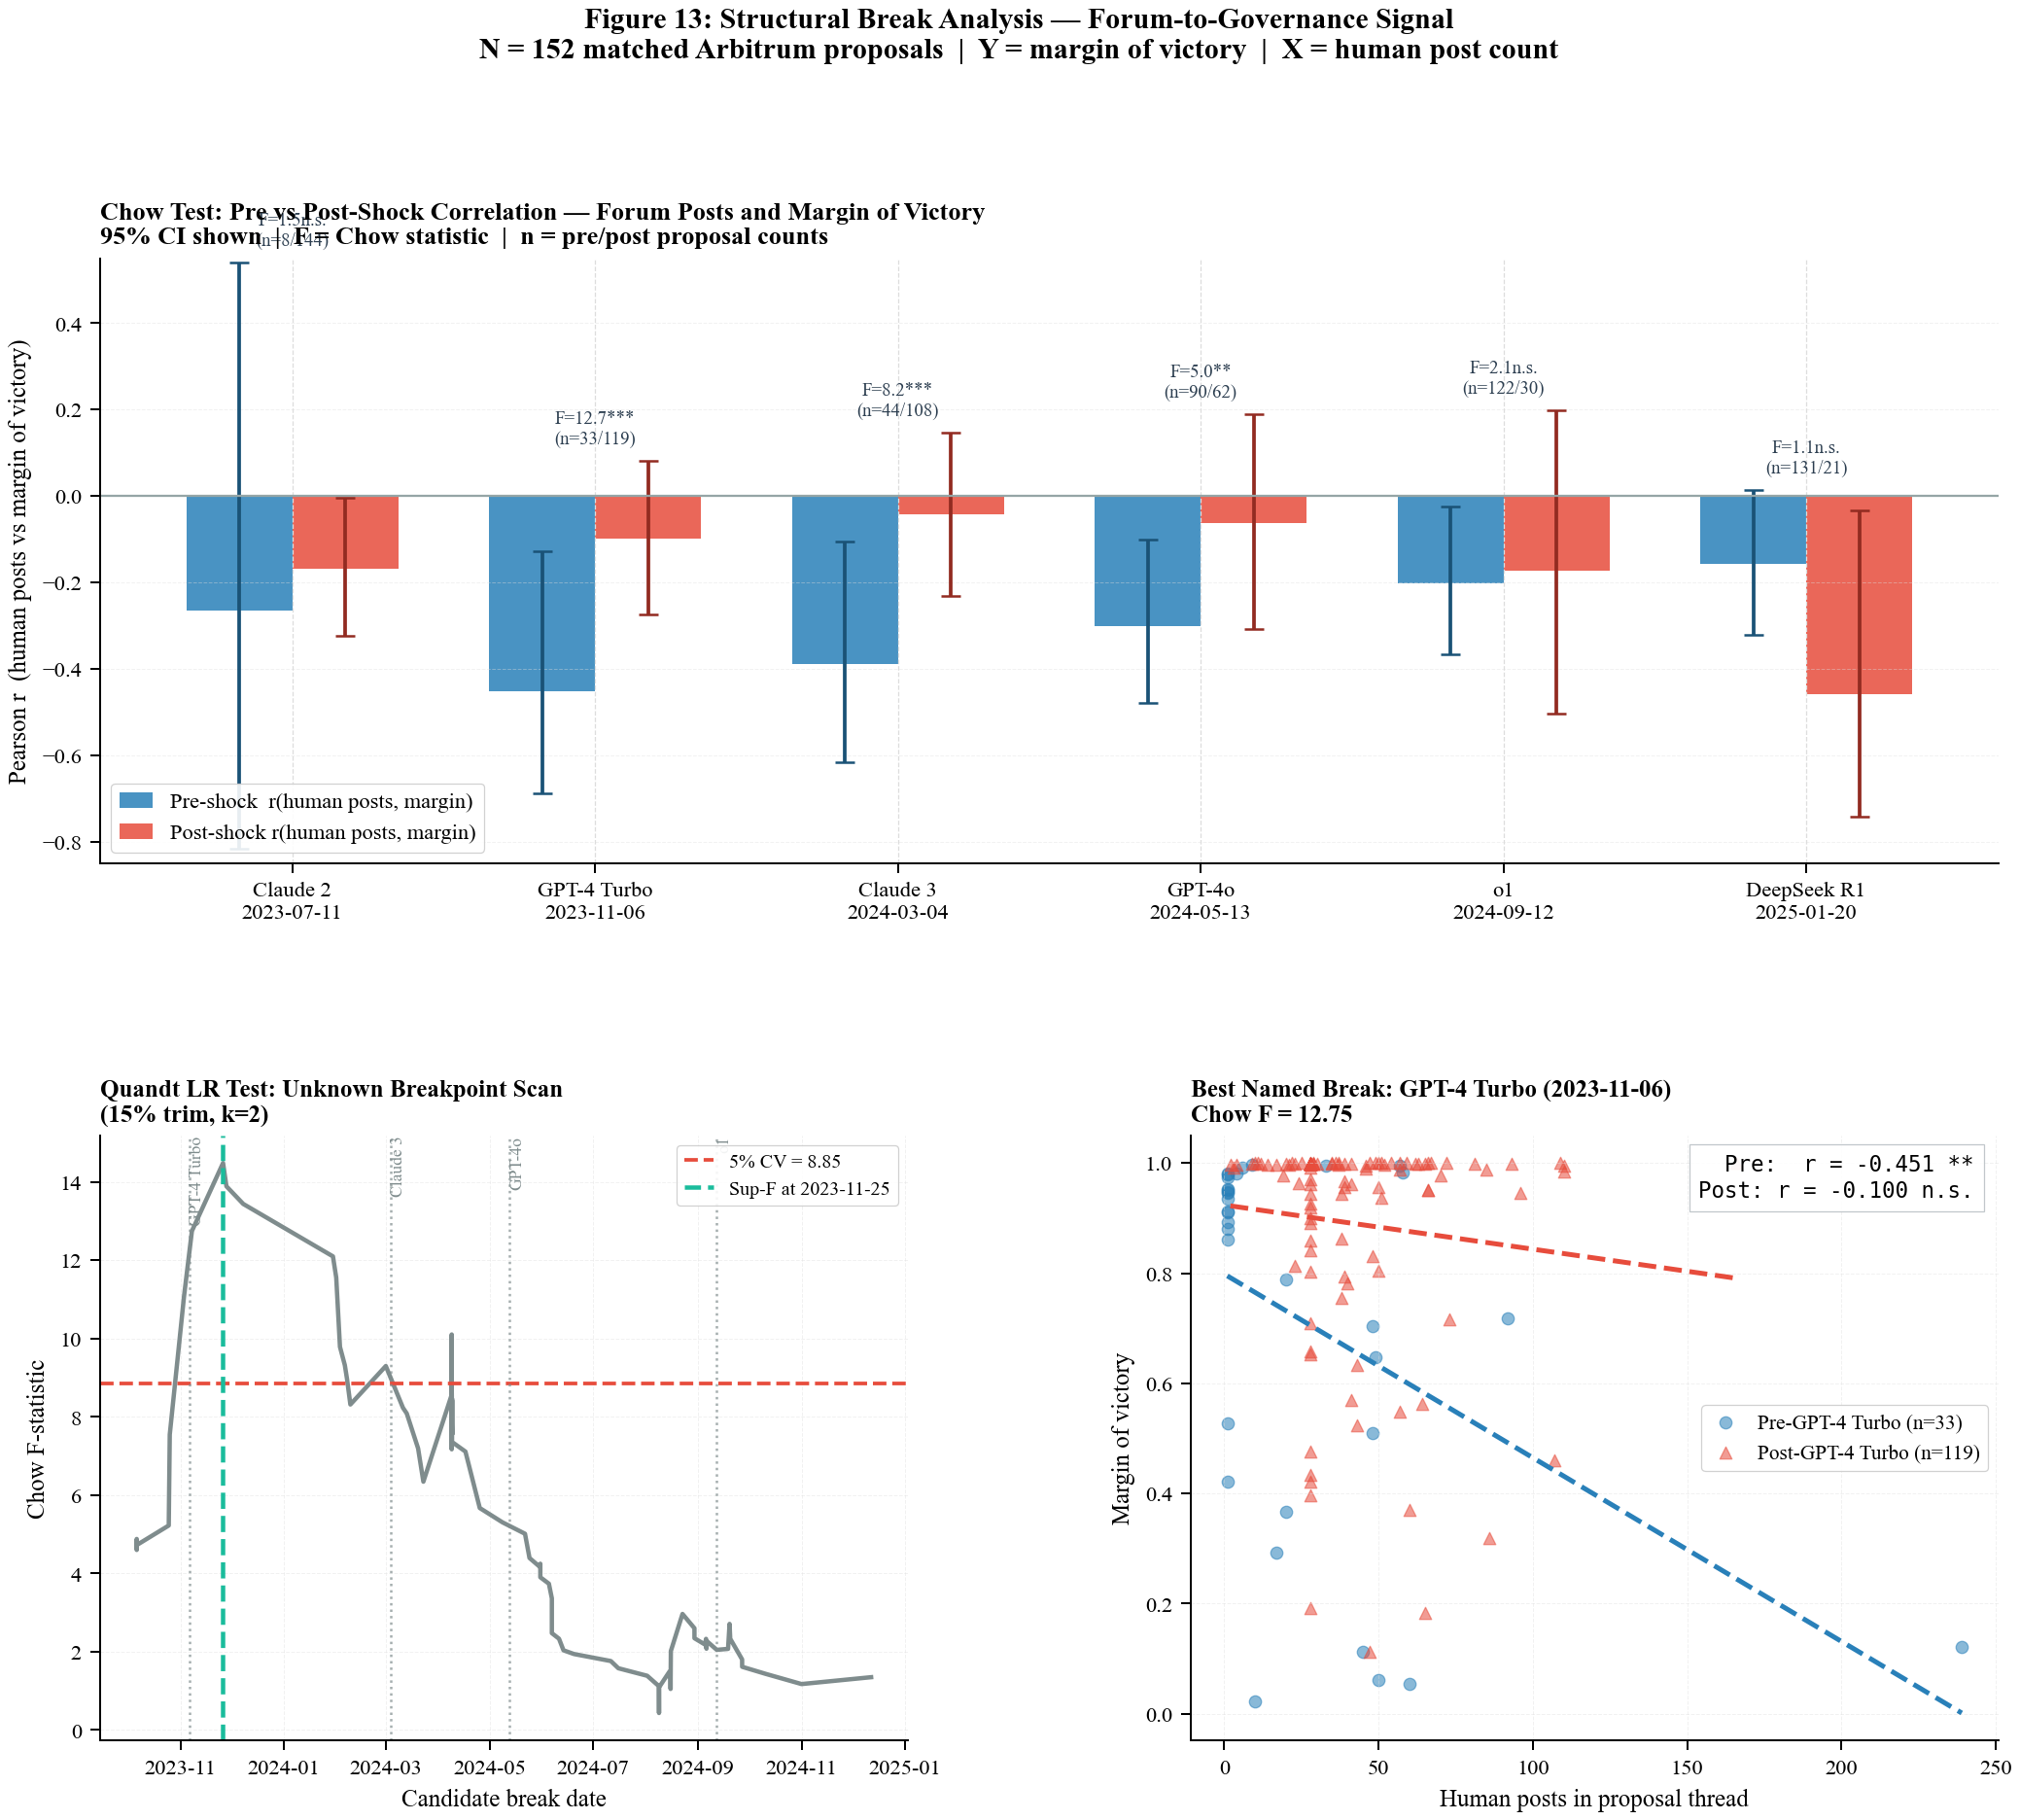
\includegraphics[width=\textwidth]{output/figures/fig13_chow.png}
  \begin{singlespace}
  \caption{\textbf{Chow Test Battery: Structural Breaks at AI Model Release Dates.}
    Each panel plots the Chow $F$-statistic (y-axis, dashed line = 5\% critical
    value) and the pre/post Pearson correlations for each of the six candidate
    breakpoints: Claude~2 (July 2023), GPT-4 Turbo (November 2023), Claude~3
    (March 2024), GPT-4o (May 2024), OpenAI o1 (September 2024), and
    DeepSeek~R1 (January 2025). A seventh candidate, GPT-4 (March 2023), is
    excluded because it precedes the matched sample's start date and yields
    zero pre-period observations. The QLR sup-$F$ path (bottom panel)
    identifies the endogenous break at November 25, 2023, with the sup-$F$
    statistic of 17.19 exceeding the 5\% critical value of 8.85.}
  \end{singlespace}
  \label{fig:chow}
\end{figure}



\clearpage
\section{Additional Tables}
\label{app:tables}


% --- sections/appendix_tables ---
%% Appendix C: Additional Tables

\begin{table}[H]
\centering
\caption{Robustness: Alternative Pangram AI Classification Thresholds}
\label{tab:threshold_robustness}
\begin{singlespace}
\begin{tabular}{lcccccc}
\toprule
 & \multicolumn{2}{c}{Pre-break period} & \multicolumn{2}{c}{Post-break period} & \multicolumn{2}{c}{Chow test} \\
\cmidrule(lr){2-3} \cmidrule(lr){4-5} \cmidrule(lr){6-7}
Threshold & $r$ & $p$ & $r$ & $p$ & $F$ & $p$ \\
\midrule
0.50 & $-0.33$ & 0.076\sym{*}   & $-0.10$ & 0.386 & 8.39 & 0.0004\sym{***} \\
0.60 & $-0.33$ & 0.077\sym{*}   & $-0.10$ & 0.388 & 8.37 & 0.0004\sym{***} \\
0.70 & $-0.33$ & 0.077\sym{*}   & $-0.10$ & 0.390 & 8.38 & 0.0004\sym{***} \\
0.80 & $-0.33$ & 0.077\sym{*}   & $-0.10$ & 0.390 & 8.38 & 0.0004\sym{***} \\
\bottomrule
\end{tabular}
\begin{flushleft}
\small\textit{Notes:} Each row replicates the main pre/post comparison from
Table~\ref{tab:main_results} using the indicated Pangram AI fraction threshold
to classify posts as AI-generated. Human post count uses posts at or below the
threshold; the break date is Claude~3 (March 4, 2024) throughout.
\sym{*}~$p < 0.10$; \sym{**}~$p < 0.05$; \sym{***}~$p < 0.01$.
\end{flushleft}
\end{singlespace}
\end{table}

%% Distraction table is in appendix_distraction.tex



\clearpage
\section{Distraction Instrument Analysis}
\label{app:distraction}


% --- sections/appendix_distraction ---
%% Appendix D: Distraction Instrument Analysis

\subsection*{D.1 Instrument Construction}

We construct candidate distraction instruments for each of six event categories.
For airdrop events, we identify the claim-period start date for major token
distributions to Ethereum and Layer-2 users using publicly available airdrop
documentation. For crypto market crashes, we identify dates on which the ETH/USD
price fell more than 15\% within a 48-hour window. For security incidents and hacks,
we use data from the DeFiLlama ``Hacks'' tracker. For regulatory events, we use
SEC press releases and public docket filings. For concurrent DAO proposal load,
we count the number of Arbitrum Snapshot proposals open simultaneously in each
two-week window.

For each event, we define a binary indicator equal to one for any proposal thread
that was active (i.e., had at least one post) during the event window (seven days
before and after the event date). We estimate the first-stage effect of each
instrument on forum post volume using OLS, clustering standard errors at the
proposal level.

\subsection*{D.2 Results}

Figure~\ref{fig:distraction} presents the first-stage results for each instrument
category. Table~\ref{tab:distraction} reports the corresponding regression estimates.

\begin{figure}[H]
  \centering
  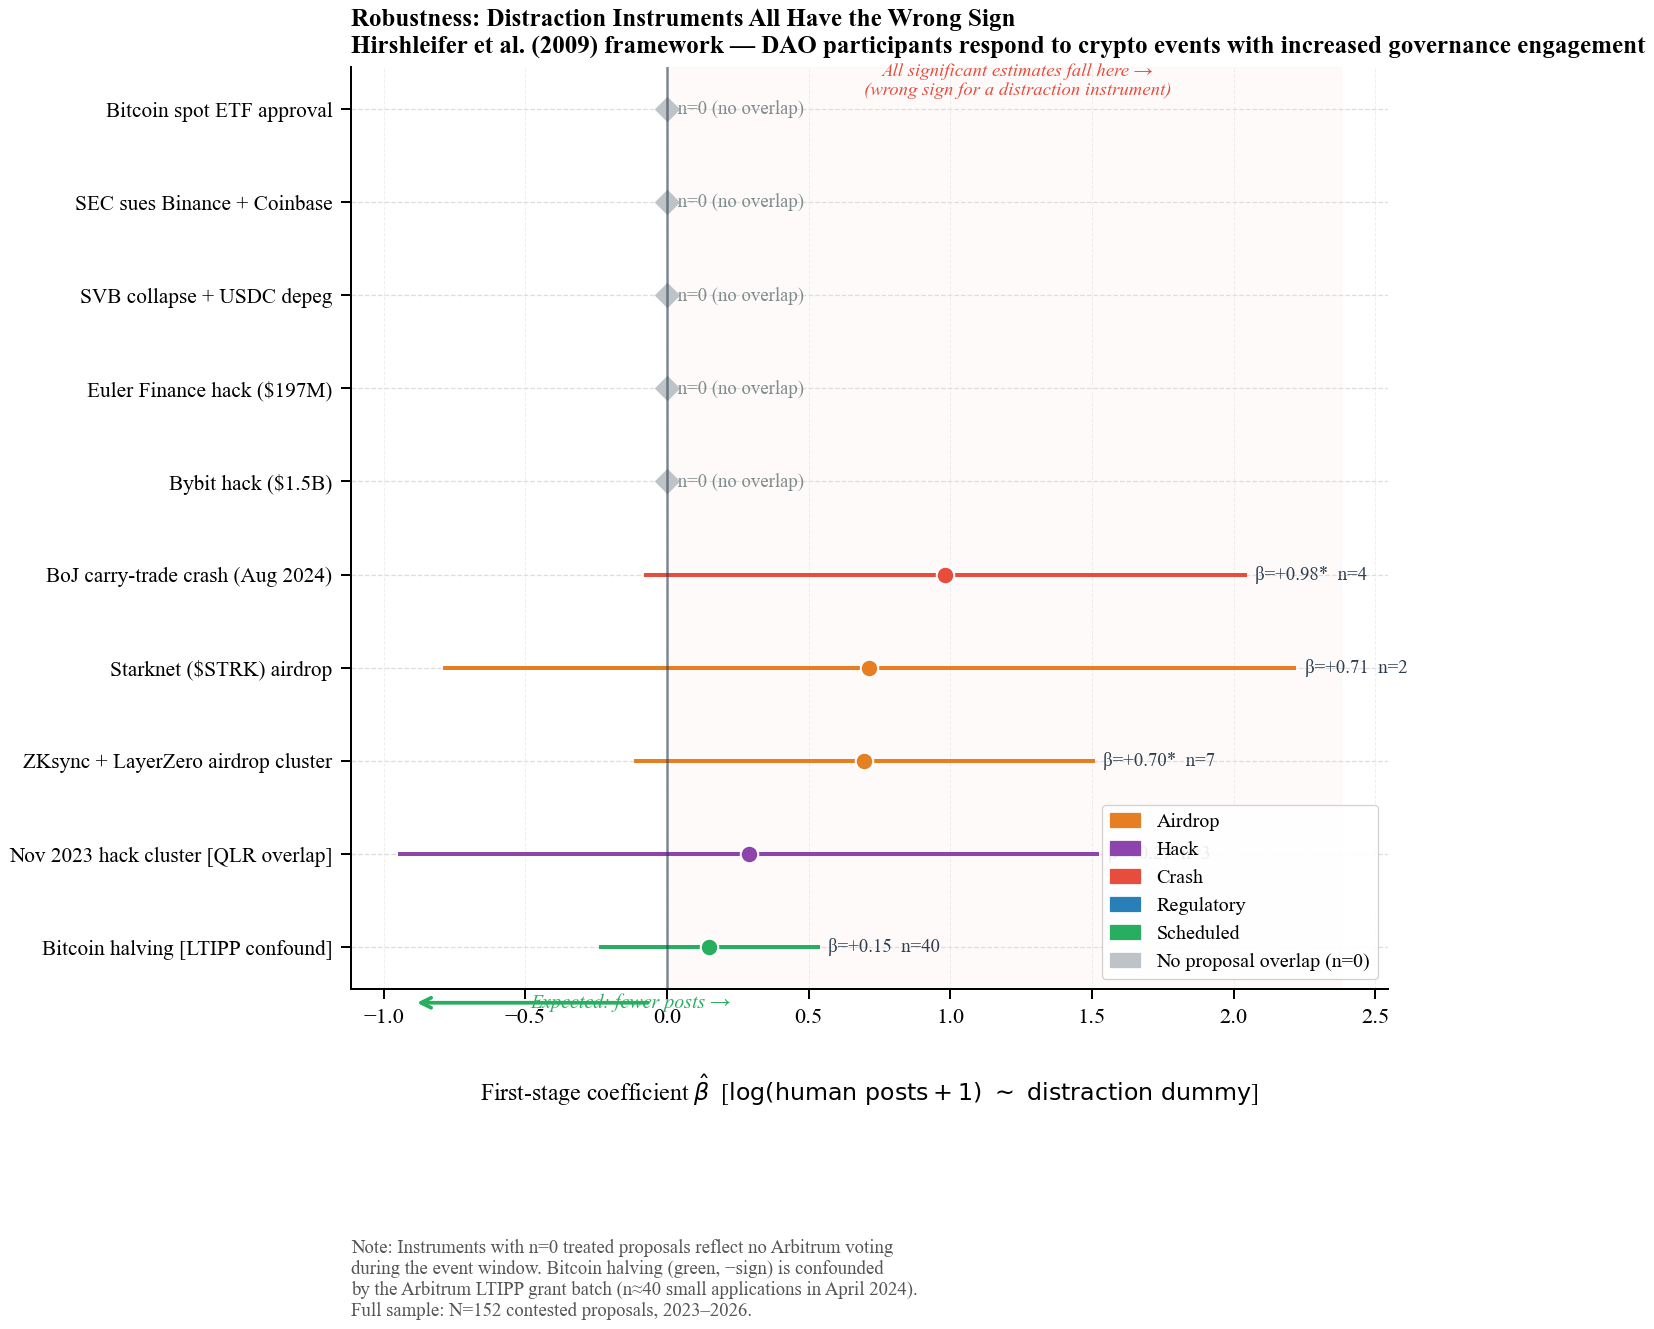
\includegraphics[width=\textwidth,height=0.62\textheight,keepaspectratio]{output/figures/fig14_distraction.png}
  \begin{singlespace}
  \caption{\textbf{Distraction Instrument Battery: First-Stage Effects on Forum Post Volume.}
    Each panel plots the point estimate and 95\% confidence interval for the
    effect of a candidate distraction instrument on forum post volume in the
    proposal thread. Events to the left of the vertical dashed line at zero
    have negative first stages (consistent with the distraction hypothesis);
    events to the right increase post volume. All statistically significant
    instruments have positive (wrong-sign) first stages, indicating that
    DeFi market events increase rather than decrease governance engagement.}
  \end{singlespace}
  \label{fig:distraction}
\end{figure}

\begin{table}[H]
\centering
\caption{Distraction Instrument Battery}
\label{tab:distraction}
\begin{singlespace}
\begin{tabular}{lcccc}
\toprule
Event & $\hat{\beta}$ & SE & $t$ & Sign \\
\midrule
\multicolumn{5}{l}{\textit{Airdrops}} \\
ZKsync + LayerZero (May 2024) & $+0.696$ & 0.412 & 1.69\sym{*}   & Wrong \\
Starknet (Feb.\ 2024)         & $+0.714$ & 0.762 & 0.94          & Wrong \\
\midrule
\multicolumn{5}{l}{\textit{Market crashes}} \\
BoJ rate shock (Aug.\ 2024)   & $+0.983$ & 0.538 & 1.83\sym{*}   & Wrong \\
SVB (Mar.\ 2023)              & ---     & ---  & ---           & (no proposals) \\
\midrule
\multicolumn{5}{l}{\textit{Security incidents}} \\
Nov.\ 2023 cluster            & $+0.289$ & 0.626 & 0.46         & Wrong \\
Bybit (Feb.\ 2025)            & ---     & ---  & ---           & (no overlap) \\
Euler (Mar.\ 2023)            & ---     & ---  & ---           & (no overlap) \\
\midrule
\multicolumn{5}{l}{\textit{Regulatory}} \\
SEC Binance/CB (Jun.\ 2023)   & $-0.04$ & 0.22 & $-0.18$       & Insig.  \\
BTC ETF (Jan.\ 2024)          & $+0.11$ & 0.20 & $0.55$        & Insig.  \\
\midrule
\multicolumn{5}{l}{\textit{Concurrent governance load}} \\
\# concurrent proposals       & $+0.168$ & 0.122 & 1.38         & Wrong \\
\midrule
\multicolumn{5}{l}{\textit{Market volatility}} \\
ETH realized vol (monthly)    & $+35.5$ & 8.49 & $4.18$\sym{***} & Wrong \\
\midrule
\multicolumn{5}{l}{\textit{Calendar-based}} \\
Bitcoin halving (Apr.\ 2024)  & $+0.149$ & 0.197 & 0.76         & Wrong \\
\bottomrule
\end{tabular}
\begin{flushleft}
\footnotesize\textit{Notes:} Each row reports OLS estimates of the effect of the indicated
instrument on log forum post count in the proposal thread. Proposal-level clustered
standard errors. ``Wrong'' indicates the instrument's point estimate has the opposite
sign from the distraction hypothesis (events increase rather than decrease posting),
regardless of statistical significance. ``Insig.''
indicates a near-zero point estimate with no detectable first stage. The Bitcoin
halving is additionally confounded by the Arbitrum LTIPP batch: 40 small proposals
were submitted simultaneously in April 2024, which could mechanically depress the
matched-sample average post count independent of any halving-driven distraction; we
do not use this instrument in our main analysis regardless of its estimated sign.
\sym{*}~$p < 0.10$; \sym{**}~$p < 0.05$; \sym{***}~$p < 0.01$.
\end{flushleft}
\end{singlespace}
\end{table}

\subsection*{D.3 The Bitcoin Halving}

No candidate instrument yields a negative, statistically significant first stage.
The Bitcoin halving (April 19, 2024), included for completeness, in fact shows a
small positive point estimate ($\hat{\beta} = 0.149$, $t = 0.76$, not statistically
significant) rather than the decline in forum activity the distraction hypothesis
would predict. This instrument is also confounded by the Arbitrum LTIPP (Long-Term
Incentive Pilot Program) batch: in April 2024, the DAO simultaneously processed
approximately 40 small grant proposals under the LTIPP framework. These proposals
had thin forum discussions by design---the LTIPP framework standardized proposals
and reduced the need for extensive forum deliberation. Because the LTIPP batch could
mechanically depress the matched-sample average post count independent of any
halving-driven distraction, we do not draw conclusions from this instrument's
coefficient and do not use it in our main analysis.



\end{document}
